\documentclass[twoside]{book}

% Packages required by doxygen
\usepackage{calc}
\usepackage{doxygen}
\usepackage{graphicx}
\usepackage[utf8]{inputenc}
\usepackage{makeidx}
\usepackage{multicol}
\usepackage{multirow}
\usepackage{fixltx2e}
\PassOptionsToPackage{warn}{textcomp}
\usepackage{textcomp}
\usepackage[nointegrals]{wasysym}
\usepackage[table]{xcolor}

% Font selection
\usepackage[T1]{fontenc}
\usepackage{mathptmx}
\usepackage[scaled=.90]{helvet}
\usepackage{courier}
\usepackage{amssymb}
\usepackage{sectsty}
\renewcommand{\familydefault}{\sfdefault}
\allsectionsfont{%
  \fontseries{bc}\selectfont%
  \color{darkgray}%
}
\renewcommand{\DoxyLabelFont}{%
  \fontseries{bc}\selectfont%
  \color{darkgray}%
}
\newcommand{\+}{\discretionary{\mbox{\scriptsize$\hookleftarrow$}}{}{}}

% Page & text layout
\usepackage{geometry}
\geometry{%
  a4paper,%
  top=2.5cm,%
  bottom=2.5cm,%
  left=2.5cm,%
  right=2.5cm%
}
\tolerance=750
\hfuzz=15pt
\hbadness=750
\setlength{\emergencystretch}{15pt}
\setlength{\parindent}{0cm}
\setlength{\parskip}{0.2cm}
\makeatletter
\renewcommand{\paragraph}{%
  \@startsection{paragraph}{4}{0ex}{-1.0ex}{1.0ex}{%
    \normalfont\normalsize\bfseries\SS@parafont%
  }%
}
\renewcommand{\subparagraph}{%
  \@startsection{subparagraph}{5}{0ex}{-1.0ex}{1.0ex}{%
    \normalfont\normalsize\bfseries\SS@subparafont%
  }%
}
\makeatother

% Headers & footers
\usepackage{fancyhdr}
\pagestyle{fancyplain}
\fancyhead[LE]{\fancyplain{}{\bfseries\thepage}}
\fancyhead[CE]{\fancyplain{}{}}
\fancyhead[RE]{\fancyplain{}{\bfseries\leftmark}}
\fancyhead[LO]{\fancyplain{}{\bfseries\rightmark}}
\fancyhead[CO]{\fancyplain{}{}}
\fancyhead[RO]{\fancyplain{}{\bfseries\thepage}}
\fancyfoot[LE]{\fancyplain{}{}}
\fancyfoot[CE]{\fancyplain{}{}}
\fancyfoot[RE]{\fancyplain{}{\bfseries\scriptsize Generated on Sun Jul 20 2014 17\+:50\+:27 for Labyrinth Game by Doxygen }}
\fancyfoot[LO]{\fancyplain{}{\bfseries\scriptsize Generated on Sun Jul 20 2014 17\+:50\+:27 for Labyrinth Game by Doxygen }}
\fancyfoot[CO]{\fancyplain{}{}}
\fancyfoot[RO]{\fancyplain{}{}}
\renewcommand{\footrulewidth}{0.4pt}
\renewcommand{\chaptermark}[1]{%
  \markboth{#1}{}%
}
\renewcommand{\sectionmark}[1]{%
  \markright{\thesection\ #1}%
}

% Indices & bibliography
\usepackage{natbib}
\usepackage[titles]{tocloft}
\setcounter{tocdepth}{3}
\setcounter{secnumdepth}{5}
\makeindex

% Hyperlinks (required, but should be loaded last)
\usepackage{ifpdf}
\ifpdf
  \usepackage[pdftex,pagebackref=true]{hyperref}
\else
  \usepackage[ps2pdf,pagebackref=true]{hyperref}
\fi
\hypersetup{%
  colorlinks=true,%
  linkcolor=blue,%
  citecolor=blue,%
  unicode%
}

% Custom commands
\newcommand{\clearemptydoublepage}{%
  \newpage{\pagestyle{empty}\cleardoublepage}%
}


%===== C O N T E N T S =====

\begin{document}

% Titlepage & ToC
\hypersetup{pageanchor=false,
             bookmarks=true,
             bookmarksnumbered=true,
             pdfencoding=unicode
            }
\pagenumbering{roman}
\begin{titlepage}
\vspace*{7cm}
\begin{center}%
{\Large Labyrinth Game }\\
\vspace*{1cm}
{\large Generated by Doxygen 1.8.7}\\
\vspace*{0.5cm}
{\small Sun Jul 20 2014 17:50:27}\\
\end{center}
\end{titlepage}
\clearemptydoublepage
\tableofcontents
\clearemptydoublepage
\pagenumbering{arabic}
\hypersetup{pageanchor=true}

%--- Begin generated contents ---
\chapter{Namespace Index}
\section{Packages}
Here are the packages with brief descriptions (if available)\+:\begin{DoxyCompactList}
\item\contentsline{section}{\hyperlink{namespace_labyrinth_game}{Labyrinth\+Game} }{\pageref{namespace_labyrinth_game}}{}
\item\contentsline{section}{\hyperlink{namespace_labyrinth_game_1_1_configuration}{Labyrinth\+Game.\+Configuration} }{\pageref{namespace_labyrinth_game_1_1_configuration}}{}
\item\contentsline{section}{\hyperlink{namespace_labyrinth_game_1_1_game_data}{Labyrinth\+Game.\+Game\+Data} }{\pageref{namespace_labyrinth_game_1_1_game_data}}{}
\item\contentsline{section}{\hyperlink{namespace_labyrinth_game_1_1_interfaces}{Labyrinth\+Game.\+Interfaces} }{\pageref{namespace_labyrinth_game_1_1_interfaces}}{}
\item\contentsline{section}{\hyperlink{namespace_labyrinth_game_1_1_labyrinths}{Labyrinth\+Game.\+Labyrinths} }{\pageref{namespace_labyrinth_game_1_1_labyrinths}}{}
\item\contentsline{section}{\hyperlink{namespace_labyrinth_game_demo}{Labyrinth\+Game\+Demo} }{\pageref{namespace_labyrinth_game_demo}}{}
\item\contentsline{section}{\hyperlink{namespace_labyrinth_game_test}{Labyrinth\+Game\+Test} }{\pageref{namespace_labyrinth_game_test}}{}
\item\contentsline{section}{\hyperlink{namespace_labyrinth_game_test_1_1_labyrinths_test}{Labyrinth\+Game\+Test.\+Labyrinths\+Test} }{\pageref{namespace_labyrinth_game_test_1_1_labyrinths_test}}{}
\end{DoxyCompactList}

\chapter{Hierarchical Index}
\section{Class Hierarchy}
This inheritance list is sorted roughly, but not completely, alphabetically\+:\begin{DoxyCompactList}
\item \contentsline{section}{Labyrinth\+Game\+Test.\+Console\+Renderer\+Test}{\pageref{class_labyrinth_game_test_1_1_console_renderer_test}}{}
\item \contentsline{section}{Labyrinth\+Game\+Test.\+Coordinate\+Test}{\pageref{class_labyrinth_game_test_1_1_coordinate_test}}{}
\item \contentsline{section}{Labyrinth\+Game\+Test.\+Labyrinths\+Test.\+Diamond\+Labyrinth\+Test}{\pageref{class_labyrinth_game_test_1_1_labyrinths_test_1_1_diamond_labyrinth_test}}{}
\item \contentsline{section}{Labyrinth\+Game\+Demo.\+Game\+Demo}{\pageref{class_labyrinth_game_demo_1_1_game_demo}}{}
\item \contentsline{section}{Labyrinth\+Game\+Test.\+Labyrinths\+Test.\+Hexagonal\+Labyrinth\+Test}{\pageref{class_labyrinth_game_test_1_1_labyrinths_test_1_1_hexagonal_labyrinth_test}}{}
\item \contentsline{section}{Labyrinth\+Game.\+Interfaces.\+I\+Coordinate}{\pageref{interface_labyrinth_game_1_1_interfaces_1_1_i_coordinate}}{}
\begin{DoxyCompactList}
\item \contentsline{section}{Labyrinth\+Game.\+Coordinate}{\pageref{class_labyrinth_game_1_1_coordinate}}{}
\end{DoxyCompactList}
\item \contentsline{section}{Labyrinth\+Game.\+Interfaces.\+I\+Labyrinth}{\pageref{interface_labyrinth_game_1_1_interfaces_1_1_i_labyrinth}}{}
\begin{DoxyCompactList}
\item \contentsline{section}{Labyrinth\+Game.\+Labyrinths.\+Labyrinth}{\pageref{class_labyrinth_game_1_1_labyrinths_1_1_labyrinth}}{}
\begin{DoxyCompactList}
\item \contentsline{section}{Labyrinth\+Game.\+Labyrinths.\+Diamond\+Labyrinth}{\pageref{class_labyrinth_game_1_1_labyrinths_1_1_diamond_labyrinth}}{}
\item \contentsline{section}{Labyrinth\+Game.\+Labyrinths.\+Hexagonal\+Labyrinth}{\pageref{class_labyrinth_game_1_1_labyrinths_1_1_hexagonal_labyrinth}}{}
\item \contentsline{section}{Labyrinth\+Game.\+Labyrinths.\+Pentagon\+Labyrinth}{\pageref{class_labyrinth_game_1_1_labyrinths_1_1_pentagon_labyrinth}}{}
\item \contentsline{section}{Labyrinth\+Game.\+Labyrinths.\+Square\+Labyrinth}{\pageref{class_labyrinth_game_1_1_labyrinths_1_1_square_labyrinth}}{}
\end{DoxyCompactList}
\end{DoxyCompactList}
\item \contentsline{section}{Labyrinth\+Game.\+Interfaces.\+I\+Labyrinth\+Creator}{\pageref{interface_labyrinth_game_1_1_interfaces_1_1_i_labyrinth_creator}}{}
\begin{DoxyCompactList}
\item \contentsline{section}{Labyrinth\+Game.\+Labyrinth\+Creator}{\pageref{class_labyrinth_game_1_1_labyrinth_creator}}{}
\end{DoxyCompactList}
\item \contentsline{section}{Labyrinth\+Game.\+Interfaces.\+I\+Labyrinth\+Engine}{\pageref{interface_labyrinth_game_1_1_interfaces_1_1_i_labyrinth_engine}}{}
\begin{DoxyCompactList}
\item \contentsline{section}{Labyrinth\+Game.\+Labyrinth\+Engine}{\pageref{class_labyrinth_game_1_1_labyrinth_engine}}{}
\end{DoxyCompactList}
\item \contentsline{section}{Labyrinth\+Game.\+Interfaces.\+I\+Menu}{\pageref{interface_labyrinth_game_1_1_interfaces_1_1_i_menu}}{}
\begin{DoxyCompactList}
\item \contentsline{section}{Labyrinth\+Game.\+Menu}{\pageref{class_labyrinth_game_1_1_menu}}{}
\end{DoxyCompactList}
\item \contentsline{section}{Labyrinth\+Game.\+Interfaces.\+I\+Player}{\pageref{interface_labyrinth_game_1_1_interfaces_1_1_i_player}}{}
\begin{DoxyCompactList}
\item \contentsline{section}{Labyrinth\+Game.\+Player}{\pageref{class_labyrinth_game_1_1_player}}{}
\end{DoxyCompactList}
\item \contentsline{section}{Labyrinth\+Game.\+Interfaces.\+I\+Random\+Char\+Provider}{\pageref{interface_labyrinth_game_1_1_interfaces_1_1_i_random_char_provider}}{}
\begin{DoxyCompactList}
\item \contentsline{section}{Labyrinth\+Game.\+Random\+Char\+Provider}{\pageref{class_labyrinth_game_1_1_random_char_provider}}{}
\end{DoxyCompactList}
\item \contentsline{section}{Labyrinth\+Game.\+Interfaces.\+I\+Renderer}{\pageref{interface_labyrinth_game_1_1_interfaces_1_1_i_renderer}}{}
\begin{DoxyCompactList}
\item \contentsline{section}{Labyrinth\+Game.\+Console\+Renderer}{\pageref{class_labyrinth_game_1_1_console_renderer}}{}
\end{DoxyCompactList}
\item \contentsline{section}{Labyrinth\+Game.\+Interfaces.\+I\+Score}{\pageref{interface_labyrinth_game_1_1_interfaces_1_1_i_score}}{}
\begin{DoxyCompactList}
\item \contentsline{section}{Labyrinth\+Game.\+Score}{\pageref{class_labyrinth_game_1_1_score}}{}
\end{DoxyCompactList}
\item \contentsline{section}{Labyrinth\+Game.\+Interfaces.\+I\+User\+Command}{\pageref{interface_labyrinth_game_1_1_interfaces_1_1_i_user_command}}{}
\begin{DoxyCompactList}
\item \contentsline{section}{Labyrinth\+Game.\+Keyboard\+Command}{\pageref{class_labyrinth_game_1_1_keyboard_command}}{}
\end{DoxyCompactList}
\item \contentsline{section}{Labyrinth\+Game\+Test.\+Keyboard\+Command\+Test}{\pageref{class_labyrinth_game_test_1_1_keyboard_command_test}}{}
\item \contentsline{section}{Labyrinth\+Game\+Test.\+Labyrinth\+Creator\+Test}{\pageref{class_labyrinth_game_test_1_1_labyrinth_creator_test}}{}
\item \contentsline{section}{Labyrinth\+Game\+Test.\+Labyrinth\+Engine\+Test}{\pageref{class_labyrinth_game_test_1_1_labyrinth_engine_test}}{}
\item \contentsline{section}{Labyrinth\+Game\+Test.\+Labyrinths\+Test.\+Labyrinth\+Test}{\pageref{class_labyrinth_game_test_1_1_labyrinths_test_1_1_labyrinth_test}}{}
\item \contentsline{section}{Labyrinth\+Game\+Test.\+Menu\+Test}{\pageref{class_labyrinth_game_test_1_1_menu_test}}{}
\item Ninject\+Module\begin{DoxyCompactList}
\item \contentsline{section}{Labyrinth\+Game.\+Configuration.\+Ninject\+Configuration}{\pageref{class_labyrinth_game_1_1_configuration_1_1_ninject_configuration}}{}
\end{DoxyCompactList}
\item \contentsline{section}{Labyrinth\+Game\+Test.\+Labyrinths\+Test.\+Pentagon\+Labyrinth\+Test}{\pageref{class_labyrinth_game_test_1_1_labyrinths_test_1_1_pentagon_labyrinth_test}}{}
\item \contentsline{section}{Labyrinth\+Game\+Test.\+Player\+Test}{\pageref{class_labyrinth_game_test_1_1_player_test}}{}
\item \contentsline{section}{Labyrinth\+Game\+Test.\+Random\+Char\+Provider\+Test}{\pageref{class_labyrinth_game_test_1_1_random_char_provider_test}}{}
\item \contentsline{section}{Labyrinth\+Game\+Test.\+Score\+Test}{\pageref{class_labyrinth_game_test_1_1_score_test}}{}
\item \contentsline{section}{Labyrinth\+Game\+Test.\+Labyrinths\+Test.\+Square\+Labyrinth\+Test}{\pageref{class_labyrinth_game_test_1_1_labyrinths_test_1_1_square_labyrinth_test}}{}
\end{DoxyCompactList}

\chapter{Class Index}
\section{Class List}
Here are the classes, structs, unions and interfaces with brief descriptions\+:\begin{DoxyCompactList}
\item\contentsline{section}{\hyperlink{class_labyrinth_game_1_1_console_renderer}{Labyrinth\+Game.\+Console\+Renderer} \\*Menages the drawing interface }{\pageref{class_labyrinth_game_1_1_console_renderer}}{}
\item\contentsline{section}{\hyperlink{class_labyrinth_game_test_1_1_console_renderer_test}{Labyrinth\+Game\+Test.\+Console\+Renderer\+Test} }{\pageref{class_labyrinth_game_test_1_1_console_renderer_test}}{}
\item\contentsline{section}{\hyperlink{class_labyrinth_game_1_1_coordinate}{Labyrinth\+Game.\+Coordinate} \\*The \hyperlink{class_labyrinth_game_1_1_coordinate}{Coordinate} class holds the coordinates which will be used from the other classes(like Player) }{\pageref{class_labyrinth_game_1_1_coordinate}}{}
\item\contentsline{section}{\hyperlink{class_labyrinth_game_test_1_1_coordinate_test}{Labyrinth\+Game\+Test.\+Coordinate\+Test} }{\pageref{class_labyrinth_game_test_1_1_coordinate_test}}{}
\item\contentsline{section}{\hyperlink{class_labyrinth_game_1_1_labyrinths_1_1_diamond_labyrinth}{Labyrinth\+Game.\+Labyrinths.\+Diamond\+Labyrinth} \\*\hyperlink{class_labyrinth_game_1_1_labyrinths_1_1_labyrinth}{Labyrinth} with shape like diamond }{\pageref{class_labyrinth_game_1_1_labyrinths_1_1_diamond_labyrinth}}{}
\item\contentsline{section}{\hyperlink{class_labyrinth_game_test_1_1_labyrinths_test_1_1_diamond_labyrinth_test}{Labyrinth\+Game\+Test.\+Labyrinths\+Test.\+Diamond\+Labyrinth\+Test} }{\pageref{class_labyrinth_game_test_1_1_labyrinths_test_1_1_diamond_labyrinth_test}}{}
\item\contentsline{section}{\hyperlink{class_labyrinth_game_demo_1_1_game_demo}{Labyrinth\+Game\+Demo.\+Game\+Demo} \\*Game demo class }{\pageref{class_labyrinth_game_demo_1_1_game_demo}}{}
\item\contentsline{section}{\hyperlink{class_labyrinth_game_1_1_labyrinths_1_1_hexagonal_labyrinth}{Labyrinth\+Game.\+Labyrinths.\+Hexagonal\+Labyrinth} \\*\hyperlink{class_labyrinth_game_1_1_labyrinths_1_1_labyrinth}{Labyrinth} with shape like hexagon }{\pageref{class_labyrinth_game_1_1_labyrinths_1_1_hexagonal_labyrinth}}{}
\item\contentsline{section}{\hyperlink{class_labyrinth_game_test_1_1_labyrinths_test_1_1_hexagonal_labyrinth_test}{Labyrinth\+Game\+Test.\+Labyrinths\+Test.\+Hexagonal\+Labyrinth\+Test} }{\pageref{class_labyrinth_game_test_1_1_labyrinths_test_1_1_hexagonal_labyrinth_test}}{}
\item\contentsline{section}{\hyperlink{interface_labyrinth_game_1_1_interfaces_1_1_i_coordinate}{Labyrinth\+Game.\+Interfaces.\+I\+Coordinate} \\*Interface which is inherited by the \hyperlink{class_labyrinth_game_1_1_coordinate}{Coordinate} class }{\pageref{interface_labyrinth_game_1_1_interfaces_1_1_i_coordinate}}{}
\item\contentsline{section}{\hyperlink{interface_labyrinth_game_1_1_interfaces_1_1_i_labyrinth}{Labyrinth\+Game.\+Interfaces.\+I\+Labyrinth} \\*Interface which is inherited by the Labyrinth class }{\pageref{interface_labyrinth_game_1_1_interfaces_1_1_i_labyrinth}}{}
\item\contentsline{section}{\hyperlink{interface_labyrinth_game_1_1_interfaces_1_1_i_labyrinth_creator}{Labyrinth\+Game.\+Interfaces.\+I\+Labyrinth\+Creator} \\*Main logic for creating labyrinth. }{\pageref{interface_labyrinth_game_1_1_interfaces_1_1_i_labyrinth_creator}}{}
\item\contentsline{section}{\hyperlink{interface_labyrinth_game_1_1_interfaces_1_1_i_labyrinth_engine}{Labyrinth\+Game.\+Interfaces.\+I\+Labyrinth\+Engine} \\*Interface which is inherited by the \hyperlink{class_labyrinth_game_1_1_labyrinth_engine}{Labyrinth\+Engine} class }{\pageref{interface_labyrinth_game_1_1_interfaces_1_1_i_labyrinth_engine}}{}
\item\contentsline{section}{\hyperlink{interface_labyrinth_game_1_1_interfaces_1_1_i_menu}{Labyrinth\+Game.\+Interfaces.\+I\+Menu} \\*Interface which is inherited by the \hyperlink{class_labyrinth_game_1_1_menu}{Menu} class }{\pageref{interface_labyrinth_game_1_1_interfaces_1_1_i_menu}}{}
\item\contentsline{section}{\hyperlink{interface_labyrinth_game_1_1_interfaces_1_1_i_player}{Labyrinth\+Game.\+Interfaces.\+I\+Player} \\*Interface which is inherited by the \hyperlink{class_labyrinth_game_1_1_player}{Player} class }{\pageref{interface_labyrinth_game_1_1_interfaces_1_1_i_player}}{}
\item\contentsline{section}{\hyperlink{interface_labyrinth_game_1_1_interfaces_1_1_i_random_char_provider}{Labyrinth\+Game.\+Interfaces.\+I\+Random\+Char\+Provider} }{\pageref{interface_labyrinth_game_1_1_interfaces_1_1_i_random_char_provider}}{}
\item\contentsline{section}{\hyperlink{interface_labyrinth_game_1_1_interfaces_1_1_i_renderer}{Labyrinth\+Game.\+Interfaces.\+I\+Renderer} \\*Interface that gives the view engine logic, is inherited by the Labyrinth class }{\pageref{interface_labyrinth_game_1_1_interfaces_1_1_i_renderer}}{}
\item\contentsline{section}{\hyperlink{interface_labyrinth_game_1_1_interfaces_1_1_i_score}{Labyrinth\+Game.\+Interfaces.\+I\+Score} \\*Interface which is inherited by the \hyperlink{class_labyrinth_game_1_1_score}{Score} class }{\pageref{interface_labyrinth_game_1_1_interfaces_1_1_i_score}}{}
\item\contentsline{section}{\hyperlink{interface_labyrinth_game_1_1_interfaces_1_1_i_user_command}{Labyrinth\+Game.\+Interfaces.\+I\+User\+Command} \\*Interface which is inherited from the \hyperlink{class_labyrinth_game_1_1_keyboard_command}{Keyboard\+Command} }{\pageref{interface_labyrinth_game_1_1_interfaces_1_1_i_user_command}}{}
\item\contentsline{section}{\hyperlink{class_labyrinth_game_1_1_keyboard_command}{Labyrinth\+Game.\+Keyboard\+Command} \\*The class manages the input from the Engine }{\pageref{class_labyrinth_game_1_1_keyboard_command}}{}
\item\contentsline{section}{\hyperlink{class_labyrinth_game_test_1_1_keyboard_command_test}{Labyrinth\+Game\+Test.\+Keyboard\+Command\+Test} }{\pageref{class_labyrinth_game_test_1_1_keyboard_command_test}}{}
\item\contentsline{section}{\hyperlink{class_labyrinth_game_1_1_labyrinths_1_1_labyrinth}{Labyrinth\+Game.\+Labyrinths.\+Labyrinth} \\*\hyperlink{class_labyrinth_game_1_1_labyrinths_1_1_labyrinth}{Labyrinth} main logic }{\pageref{class_labyrinth_game_1_1_labyrinths_1_1_labyrinth}}{}
\item\contentsline{section}{\hyperlink{class_labyrinth_game_1_1_labyrinth_creator}{Labyrinth\+Game.\+Labyrinth\+Creator} \\*Labyrinth creator class. Builder pattern used and this class acts as a Director }{\pageref{class_labyrinth_game_1_1_labyrinth_creator}}{}
\item\contentsline{section}{\hyperlink{class_labyrinth_game_test_1_1_labyrinth_creator_test}{Labyrinth\+Game\+Test.\+Labyrinth\+Creator\+Test} }{\pageref{class_labyrinth_game_test_1_1_labyrinth_creator_test}}{}
\item\contentsline{section}{\hyperlink{class_labyrinth_game_1_1_labyrinth_engine}{Labyrinth\+Game.\+Labyrinth\+Engine} \\*Singleton implementation of the game engine }{\pageref{class_labyrinth_game_1_1_labyrinth_engine}}{}
\item\contentsline{section}{\hyperlink{class_labyrinth_game_test_1_1_labyrinth_engine_test}{Labyrinth\+Game\+Test.\+Labyrinth\+Engine\+Test} }{\pageref{class_labyrinth_game_test_1_1_labyrinth_engine_test}}{}
\item\contentsline{section}{\hyperlink{class_labyrinth_game_test_1_1_labyrinths_test_1_1_labyrinth_test}{Labyrinth\+Game\+Test.\+Labyrinths\+Test.\+Labyrinth\+Test} }{\pageref{class_labyrinth_game_test_1_1_labyrinths_test_1_1_labyrinth_test}}{}
\item\contentsline{section}{\hyperlink{class_labyrinth_game_1_1_menu}{Labyrinth\+Game.\+Menu} \\*The \hyperlink{class_labyrinth_game_1_1_menu}{Menu} class holds the info about the menu of the game }{\pageref{class_labyrinth_game_1_1_menu}}{}
\item\contentsline{section}{\hyperlink{class_labyrinth_game_test_1_1_menu_test}{Labyrinth\+Game\+Test.\+Menu\+Test} }{\pageref{class_labyrinth_game_test_1_1_menu_test}}{}
\item\contentsline{section}{\hyperlink{class_labyrinth_game_1_1_configuration_1_1_ninject_configuration}{Labyrinth\+Game.\+Configuration.\+Ninject\+Configuration} }{\pageref{class_labyrinth_game_1_1_configuration_1_1_ninject_configuration}}{}
\item\contentsline{section}{\hyperlink{class_labyrinth_game_1_1_labyrinths_1_1_pentagon_labyrinth}{Labyrinth\+Game.\+Labyrinths.\+Pentagon\+Labyrinth} \\*Pentagon shaped labyrinth }{\pageref{class_labyrinth_game_1_1_labyrinths_1_1_pentagon_labyrinth}}{}
\item\contentsline{section}{\hyperlink{class_labyrinth_game_test_1_1_labyrinths_test_1_1_pentagon_labyrinth_test}{Labyrinth\+Game\+Test.\+Labyrinths\+Test.\+Pentagon\+Labyrinth\+Test} }{\pageref{class_labyrinth_game_test_1_1_labyrinths_test_1_1_pentagon_labyrinth_test}}{}
\item\contentsline{section}{\hyperlink{class_labyrinth_game_1_1_player}{Labyrinth\+Game.\+Player} \\*The \hyperlink{class_labyrinth_game_1_1_player}{Player} class hold information about start position, player name and points }{\pageref{class_labyrinth_game_1_1_player}}{}
\item\contentsline{section}{\hyperlink{class_labyrinth_game_test_1_1_player_test}{Labyrinth\+Game\+Test.\+Player\+Test} }{\pageref{class_labyrinth_game_test_1_1_player_test}}{}
\item\contentsline{section}{\hyperlink{class_labyrinth_game_1_1_random_char_provider}{Labyrinth\+Game.\+Random\+Char\+Provider} }{\pageref{class_labyrinth_game_1_1_random_char_provider}}{}
\item\contentsline{section}{\hyperlink{class_labyrinth_game_test_1_1_random_char_provider_test}{Labyrinth\+Game\+Test.\+Random\+Char\+Provider\+Test} }{\pageref{class_labyrinth_game_test_1_1_random_char_provider_test}}{}
\item\contentsline{section}{\hyperlink{class_labyrinth_game_1_1_score}{Labyrinth\+Game.\+Score} \\*\hyperlink{class_labyrinth_game_1_1_score}{Score} class keeps player name and achieved result }{\pageref{class_labyrinth_game_1_1_score}}{}
\item\contentsline{section}{\hyperlink{class_labyrinth_game_test_1_1_score_test}{Labyrinth\+Game\+Test.\+Score\+Test} }{\pageref{class_labyrinth_game_test_1_1_score_test}}{}
\item\contentsline{section}{\hyperlink{class_labyrinth_game_1_1_labyrinths_1_1_square_labyrinth}{Labyrinth\+Game.\+Labyrinths.\+Square\+Labyrinth} \\*\hyperlink{class_labyrinth_game_1_1_labyrinths_1_1_labyrinth}{Labyrinth} with square shape }{\pageref{class_labyrinth_game_1_1_labyrinths_1_1_square_labyrinth}}{}
\item\contentsline{section}{\hyperlink{class_labyrinth_game_test_1_1_labyrinths_test_1_1_square_labyrinth_test}{Labyrinth\+Game\+Test.\+Labyrinths\+Test.\+Square\+Labyrinth\+Test} }{\pageref{class_labyrinth_game_test_1_1_labyrinths_test_1_1_square_labyrinth_test}}{}
\end{DoxyCompactList}

\chapter{Namespace Documentation}
\hypertarget{namespace_labyrinth_game}{\section{Package Labyrinth\+Game}
\label{namespace_labyrinth_game}\index{Labyrinth\+Game@{Labyrinth\+Game}}
}
\subsection*{Namespaces}
\begin{DoxyCompactItemize}
\item 
package \hyperlink{namespace_labyrinth_game_1_1_configuration}{Configuration}
\item 
package \hyperlink{namespace_labyrinth_game_1_1_game_data}{Game\+Data}
\item 
package \hyperlink{namespace_labyrinth_game_1_1_interfaces}{Interfaces}
\item 
package \hyperlink{namespace_labyrinth_game_1_1_labyrinths}{Labyrinths}
\end{DoxyCompactItemize}
\subsection*{Classes}
\begin{DoxyCompactItemize}
\item 
class \hyperlink{class_labyrinth_game_1_1_console_renderer}{Console\+Renderer}
\begin{DoxyCompactList}\small\item\em Menages the drawing interface \end{DoxyCompactList}\item 
class \hyperlink{class_labyrinth_game_1_1_coordinate}{Coordinate}
\begin{DoxyCompactList}\small\item\em The \hyperlink{class_labyrinth_game_1_1_coordinate}{Coordinate} class holds the coordinates which will be used from the other classes(like Player) \end{DoxyCompactList}\item 
class \hyperlink{class_labyrinth_game_1_1_keyboard_command}{Keyboard\+Command}
\begin{DoxyCompactList}\small\item\em The class manages the input from the Engine \end{DoxyCompactList}\item 
class \hyperlink{class_labyrinth_game_1_1_labyrinth_creator}{Labyrinth\+Creator}
\begin{DoxyCompactList}\small\item\em Labyrinth creator class. Builder pattern used and this class acts as a Director \end{DoxyCompactList}\item 
class \hyperlink{class_labyrinth_game_1_1_labyrinth_engine}{Labyrinth\+Engine}
\begin{DoxyCompactList}\small\item\em Singleton implementation of the game engine \end{DoxyCompactList}\item 
class \hyperlink{class_labyrinth_game_1_1_menu}{Menu}
\begin{DoxyCompactList}\small\item\em The \hyperlink{class_labyrinth_game_1_1_menu}{Menu} class holds the info about the menu of the game \end{DoxyCompactList}\item 
class \hyperlink{class_labyrinth_game_1_1_player}{Player}
\begin{DoxyCompactList}\small\item\em The \hyperlink{class_labyrinth_game_1_1_player}{Player} class hold information about start position, player name and points \end{DoxyCompactList}\item 
class \hyperlink{class_labyrinth_game_1_1_random_char_provider}{Random\+Char\+Provider}
\item 
class \hyperlink{class_labyrinth_game_1_1_score}{Score}
\begin{DoxyCompactList}\small\item\em \hyperlink{class_labyrinth_game_1_1_score}{Score} class keeps player name and achieved result \end{DoxyCompactList}\end{DoxyCompactItemize}

\hypertarget{namespace_labyrinth_game_1_1_configuration}{\section{Package Labyrinth\+Game.\+Configuration}
\label{namespace_labyrinth_game_1_1_configuration}\index{Labyrinth\+Game.\+Configuration@{Labyrinth\+Game.\+Configuration}}
}
\subsection*{Classes}
\begin{DoxyCompactItemize}
\item 
class \hyperlink{class_labyrinth_game_1_1_configuration_1_1_ninject_configuration}{Ninject\+Configuration}
\end{DoxyCompactItemize}

\hypertarget{namespace_labyrinth_game_1_1_game_data}{\section{Package Labyrinth\+Game.\+Game\+Data}
\label{namespace_labyrinth_game_1_1_game_data}\index{Labyrinth\+Game.\+Game\+Data@{Labyrinth\+Game.\+Game\+Data}}
}
\subsection*{Enumerations}
\begin{DoxyCompactItemize}
\item 
enum \hyperlink{namespace_labyrinth_game_1_1_game_data_a669d2cc2c6f5f970d09157d0b7fd6c70}{Symbol} \{ {\bfseries Obstacle} = '$\ast$', 
{\bfseries Path} = '-\/', 
{\bfseries Blank\+Space} = '.', 
{\bfseries Player} = 'X'
 \}
\begin{DoxyCompactList}\small\item\em Enumeration containing the specific symbols used in the labyrinths \end{DoxyCompactList}\item 
enum \hyperlink{namespace_labyrinth_game_1_1_game_data_a911877be7f3c2eb330b648e52945476c}{Type\+Labyrinth} \{ {\bfseries Diamond}, 
{\bfseries Pentagram}, 
{\bfseries Hexagon}, 
{\bfseries Square}
 \}
\begin{DoxyCompactList}\small\item\em Enumeration containing the specific type of the labyrinths \end{DoxyCompactList}\end{DoxyCompactItemize}


\subsection{Enumeration Type Documentation}
\hypertarget{namespace_labyrinth_game_1_1_game_data_a669d2cc2c6f5f970d09157d0b7fd6c70}{\index{Labyrinth\+Game\+::\+Game\+Data@{Labyrinth\+Game\+::\+Game\+Data}!Symbol@{Symbol}}
\index{Symbol@{Symbol}!Labyrinth\+Game\+::\+Game\+Data@{Labyrinth\+Game\+::\+Game\+Data}}
\subsubsection[{Symbol}]{\setlength{\rightskip}{0pt plus 5cm}enum {\bf Labyrinth\+Game.\+Game\+Data.\+Symbol}}}\label{namespace_labyrinth_game_1_1_game_data_a669d2cc2c6f5f970d09157d0b7fd6c70}


Enumeration containing the specific symbols used in the labyrinths 



Definition at line 6 of file Symbol.\+cs.

\hypertarget{namespace_labyrinth_game_1_1_game_data_a911877be7f3c2eb330b648e52945476c}{\index{Labyrinth\+Game\+::\+Game\+Data@{Labyrinth\+Game\+::\+Game\+Data}!Type\+Labyrinth@{Type\+Labyrinth}}
\index{Type\+Labyrinth@{Type\+Labyrinth}!Labyrinth\+Game\+::\+Game\+Data@{Labyrinth\+Game\+::\+Game\+Data}}
\subsubsection[{Type\+Labyrinth}]{\setlength{\rightskip}{0pt plus 5cm}enum {\bf Labyrinth\+Game.\+Game\+Data.\+Type\+Labyrinth}}}\label{namespace_labyrinth_game_1_1_game_data_a911877be7f3c2eb330b648e52945476c}


Enumeration containing the specific type of the labyrinths 



Definition at line 6 of file Type\+Labyrinth.\+cs.


\hypertarget{namespace_labyrinth_game_1_1_interfaces}{\section{Package Labyrinth\+Game.\+Interfaces}
\label{namespace_labyrinth_game_1_1_interfaces}\index{Labyrinth\+Game.\+Interfaces@{Labyrinth\+Game.\+Interfaces}}
}
\subsection*{Classes}
\begin{DoxyCompactItemize}
\item 
interface \hyperlink{interface_labyrinth_game_1_1_interfaces_1_1_i_coordinate}{I\+Coordinate}
\begin{DoxyCompactList}\small\item\em Interface which is inherited by the \hyperlink{class_labyrinth_game_1_1_coordinate}{Coordinate} class \end{DoxyCompactList}\item 
interface \hyperlink{interface_labyrinth_game_1_1_interfaces_1_1_i_labyrinth}{I\+Labyrinth}
\begin{DoxyCompactList}\small\item\em Interface which is inherited by the Labyrinth class \end{DoxyCompactList}\item 
interface \hyperlink{interface_labyrinth_game_1_1_interfaces_1_1_i_labyrinth_creator}{I\+Labyrinth\+Creator}
\begin{DoxyCompactList}\small\item\em Main logic for creating labyrinth. \end{DoxyCompactList}\item 
interface \hyperlink{interface_labyrinth_game_1_1_interfaces_1_1_i_labyrinth_engine}{I\+Labyrinth\+Engine}
\begin{DoxyCompactList}\small\item\em Interface which is inherited by the \hyperlink{class_labyrinth_game_1_1_labyrinth_engine}{Labyrinth\+Engine} class \end{DoxyCompactList}\item 
interface \hyperlink{interface_labyrinth_game_1_1_interfaces_1_1_i_menu}{I\+Menu}
\begin{DoxyCompactList}\small\item\em Interface which is inherited by the \hyperlink{class_labyrinth_game_1_1_menu}{Menu} class \end{DoxyCompactList}\item 
interface \hyperlink{interface_labyrinth_game_1_1_interfaces_1_1_i_player}{I\+Player}
\begin{DoxyCompactList}\small\item\em Interface which is inherited by the \hyperlink{class_labyrinth_game_1_1_player}{Player} class \end{DoxyCompactList}\item 
interface \hyperlink{interface_labyrinth_game_1_1_interfaces_1_1_i_random_char_provider}{I\+Random\+Char\+Provider}
\item 
interface \hyperlink{interface_labyrinth_game_1_1_interfaces_1_1_i_renderer}{I\+Renderer}
\begin{DoxyCompactList}\small\item\em Interface that gives the view engine logic, is inherited by the Labyrinth class \end{DoxyCompactList}\item 
interface \hyperlink{interface_labyrinth_game_1_1_interfaces_1_1_i_score}{I\+Score}
\begin{DoxyCompactList}\small\item\em Interface which is inherited by the \hyperlink{class_labyrinth_game_1_1_score}{Score} class \end{DoxyCompactList}\item 
interface \hyperlink{interface_labyrinth_game_1_1_interfaces_1_1_i_user_command}{I\+User\+Command}
\begin{DoxyCompactList}\small\item\em Interface which is inherited from the \hyperlink{class_labyrinth_game_1_1_keyboard_command}{Keyboard\+Command} \end{DoxyCompactList}\end{DoxyCompactItemize}

\hypertarget{namespace_labyrinth_game_1_1_labyrinths}{\section{Package Labyrinth\+Game.\+Labyrinths}
\label{namespace_labyrinth_game_1_1_labyrinths}\index{Labyrinth\+Game.\+Labyrinths@{Labyrinth\+Game.\+Labyrinths}}
}
\subsection*{Classes}
\begin{DoxyCompactItemize}
\item 
class \hyperlink{class_labyrinth_game_1_1_labyrinths_1_1_diamond_labyrinth}{Diamond\+Labyrinth}
\begin{DoxyCompactList}\small\item\em \hyperlink{class_labyrinth_game_1_1_labyrinths_1_1_labyrinth}{Labyrinth} with shape like diamond \end{DoxyCompactList}\item 
class \hyperlink{class_labyrinth_game_1_1_labyrinths_1_1_hexagonal_labyrinth}{Hexagonal\+Labyrinth}
\begin{DoxyCompactList}\small\item\em \hyperlink{class_labyrinth_game_1_1_labyrinths_1_1_labyrinth}{Labyrinth} with shape like hexagon \end{DoxyCompactList}\item 
class \hyperlink{class_labyrinth_game_1_1_labyrinths_1_1_labyrinth}{Labyrinth}
\begin{DoxyCompactList}\small\item\em \hyperlink{class_labyrinth_game_1_1_labyrinths_1_1_labyrinth}{Labyrinth} main logic \end{DoxyCompactList}\item 
class \hyperlink{class_labyrinth_game_1_1_labyrinths_1_1_pentagon_labyrinth}{Pentagon\+Labyrinth}
\begin{DoxyCompactList}\small\item\em Pentagon shaped labyrinth \end{DoxyCompactList}\item 
class \hyperlink{class_labyrinth_game_1_1_labyrinths_1_1_square_labyrinth}{Square\+Labyrinth}
\begin{DoxyCompactList}\small\item\em \hyperlink{class_labyrinth_game_1_1_labyrinths_1_1_labyrinth}{Labyrinth} with square shape \end{DoxyCompactList}\end{DoxyCompactItemize}

\hypertarget{namespace_labyrinth_game_demo}{\section{Package Labyrinth\+Game\+Demo}
\label{namespace_labyrinth_game_demo}\index{Labyrinth\+Game\+Demo@{Labyrinth\+Game\+Demo}}
}
\subsection*{Classes}
\begin{DoxyCompactItemize}
\item 
class \hyperlink{class_labyrinth_game_demo_1_1_game_demo}{Game\+Demo}
\begin{DoxyCompactList}\small\item\em Game demo class \end{DoxyCompactList}\end{DoxyCompactItemize}

\hypertarget{namespace_labyrinth_game_test}{\section{Package Labyrinth\+Game\+Test}
\label{namespace_labyrinth_game_test}\index{Labyrinth\+Game\+Test@{Labyrinth\+Game\+Test}}
}
\subsection*{Namespaces}
\begin{DoxyCompactItemize}
\item 
package \hyperlink{namespace_labyrinth_game_test_1_1_labyrinths_test}{Labyrinths\+Test}
\end{DoxyCompactItemize}
\subsection*{Classes}
\begin{DoxyCompactItemize}
\item 
class \hyperlink{class_labyrinth_game_test_1_1_console_renderer_test}{Console\+Renderer\+Test}
\item 
class \hyperlink{class_labyrinth_game_test_1_1_coordinate_test}{Coordinate\+Test}
\item 
class \hyperlink{class_labyrinth_game_test_1_1_keyboard_command_test}{Keyboard\+Command\+Test}
\item 
class \hyperlink{class_labyrinth_game_test_1_1_labyrinth_creator_test}{Labyrinth\+Creator\+Test}
\item 
class \hyperlink{class_labyrinth_game_test_1_1_labyrinth_engine_test}{Labyrinth\+Engine\+Test}
\item 
class \hyperlink{class_labyrinth_game_test_1_1_menu_test}{Menu\+Test}
\item 
class \hyperlink{class_labyrinth_game_test_1_1_player_test}{Player\+Test}
\item 
class \hyperlink{class_labyrinth_game_test_1_1_random_char_provider_test}{Random\+Char\+Provider\+Test}
\item 
class \hyperlink{class_labyrinth_game_test_1_1_score_test}{Score\+Test}
\end{DoxyCompactItemize}

\hypertarget{namespace_labyrinth_game_test_1_1_labyrinths_test}{\section{Package Labyrinth\+Game\+Test.\+Labyrinths\+Test}
\label{namespace_labyrinth_game_test_1_1_labyrinths_test}\index{Labyrinth\+Game\+Test.\+Labyrinths\+Test@{Labyrinth\+Game\+Test.\+Labyrinths\+Test}}
}
\subsection*{Classes}
\begin{DoxyCompactItemize}
\item 
class \hyperlink{class_labyrinth_game_test_1_1_labyrinths_test_1_1_diamond_labyrinth_test}{Diamond\+Labyrinth\+Test}
\item 
class \hyperlink{class_labyrinth_game_test_1_1_labyrinths_test_1_1_hexagonal_labyrinth_test}{Hexagonal\+Labyrinth\+Test}
\item 
class \hyperlink{class_labyrinth_game_test_1_1_labyrinths_test_1_1_labyrinth_test}{Labyrinth\+Test}
\item 
class \hyperlink{class_labyrinth_game_test_1_1_labyrinths_test_1_1_pentagon_labyrinth_test}{Pentagon\+Labyrinth\+Test}
\item 
class \hyperlink{class_labyrinth_game_test_1_1_labyrinths_test_1_1_square_labyrinth_test}{Square\+Labyrinth\+Test}
\end{DoxyCompactItemize}

\chapter{Class Documentation}
\hypertarget{class_labyrinth_game_1_1_console_renderer}{\section{Labyrinth\+Game.\+Console\+Renderer Class Reference}
\label{class_labyrinth_game_1_1_console_renderer}\index{Labyrinth\+Game.\+Console\+Renderer@{Labyrinth\+Game.\+Console\+Renderer}}
}


Menages the drawing interface  


Inheritance diagram for Labyrinth\+Game.\+Console\+Renderer\+:\begin{figure}[H]
\begin{center}
\leavevmode
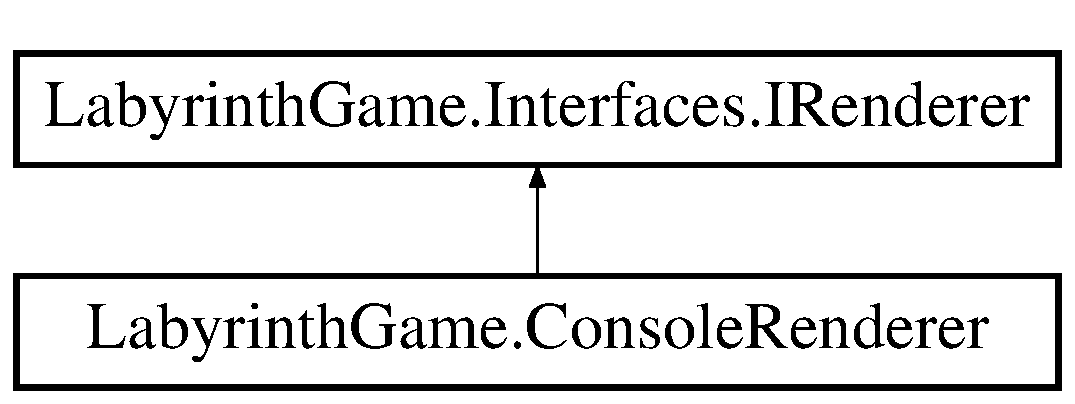
\includegraphics[height=2.000000cm]{class_labyrinth_game_1_1_console_renderer}
\end{center}
\end{figure}
\subsection*{Public Member Functions}
\begin{DoxyCompactItemize}
\item 
virtual void \hyperlink{class_labyrinth_game_1_1_console_renderer_a4e1d4a210c07a261d5dbca5b471a2300}{Render} (\hyperlink{interface_labyrinth_game_1_1_interfaces_1_1_i_labyrinth}{I\+Labyrinth} labyrinth)
\begin{DoxyCompactList}\small\item\em This method gives each symbol a specific color to render on the console \end{DoxyCompactList}\end{DoxyCompactItemize}


\subsection{Detailed Description}
Menages the drawing interface 



Definition at line 10 of file Console\+Renderer.\+cs.



\subsection{Member Function Documentation}
\hypertarget{class_labyrinth_game_1_1_console_renderer_a4e1d4a210c07a261d5dbca5b471a2300}{\index{Labyrinth\+Game\+::\+Console\+Renderer@{Labyrinth\+Game\+::\+Console\+Renderer}!Render@{Render}}
\index{Render@{Render}!Labyrinth\+Game\+::\+Console\+Renderer@{Labyrinth\+Game\+::\+Console\+Renderer}}
\subsubsection[{Render}]{\setlength{\rightskip}{0pt plus 5cm}virtual void Labyrinth\+Game.\+Console\+Renderer.\+Render (
\begin{DoxyParamCaption}
\item[{{\bf I\+Labyrinth}}]{labyrinth}
\end{DoxyParamCaption}
)\hspace{0.3cm}{\ttfamily [virtual]}}}\label{class_labyrinth_game_1_1_console_renderer_a4e1d4a210c07a261d5dbca5b471a2300}


This method gives each symbol a specific color to render on the console 



Implements \hyperlink{interface_labyrinth_game_1_1_interfaces_1_1_i_renderer}{Labyrinth\+Game.\+Interfaces.\+I\+Renderer}.



Definition at line 15 of file Console\+Renderer.\+cs.



The documentation for this class was generated from the following file\+:\begin{DoxyCompactItemize}
\item 
Labyrinth\+Game/Console\+Renderer.\+cs\end{DoxyCompactItemize}

\hypertarget{class_labyrinth_game_test_1_1_console_renderer_test}{\section{Labyrinth\+Game\+Test.\+Console\+Renderer\+Test Class Reference}
\label{class_labyrinth_game_test_1_1_console_renderer_test}\index{Labyrinth\+Game\+Test.\+Console\+Renderer\+Test@{Labyrinth\+Game\+Test.\+Console\+Renderer\+Test}}
}
\subsection*{Public Member Functions}
\begin{DoxyCompactItemize}
\item 
\hypertarget{class_labyrinth_game_test_1_1_console_renderer_test_ad98f26fcb9e686508658c69ab32036cc}{void {\bfseries Render\+Diamond\+Labyrinth\+Test} ()}\label{class_labyrinth_game_test_1_1_console_renderer_test_ad98f26fcb9e686508658c69ab32036cc}

\item 
\hypertarget{class_labyrinth_game_test_1_1_console_renderer_test_aa29f763eeac769af7c9c5d165730e24e}{void {\bfseries Render\+Hexadiagonal\+Labyrinth\+Test} ()}\label{class_labyrinth_game_test_1_1_console_renderer_test_aa29f763eeac769af7c9c5d165730e24e}

\item 
\hypertarget{class_labyrinth_game_test_1_1_console_renderer_test_ace0b60bc7a78e61ce25b228e9fd579af}{void {\bfseries Render\+Pentagon\+Labyrinth\+Test} ()}\label{class_labyrinth_game_test_1_1_console_renderer_test_ace0b60bc7a78e61ce25b228e9fd579af}

\item 
\hypertarget{class_labyrinth_game_test_1_1_console_renderer_test_a381b5a3466c60c5c66dda0667cf65cb7}{void {\bfseries Render\+Square\+Labyrinth\+Test} ()}\label{class_labyrinth_game_test_1_1_console_renderer_test_a381b5a3466c60c5c66dda0667cf65cb7}

\end{DoxyCompactItemize}
\subsection*{Static Public Member Functions}
\begin{DoxyCompactItemize}
\item 
\hypertarget{class_labyrinth_game_test_1_1_console_renderer_test_a638c8b5ff7ebd1657ab7304a1563535c}{static void {\bfseries Console\+Renderer\+Class\+Inicialize} (Test\+Context test\+Context)}\label{class_labyrinth_game_test_1_1_console_renderer_test_a638c8b5ff7ebd1657ab7304a1563535c}

\end{DoxyCompactItemize}


\subsection{Detailed Description}


Definition at line 11 of file Console\+Renderer\+Test.\+cs.



The documentation for this class was generated from the following file\+:\begin{DoxyCompactItemize}
\item 
Labyrinth\+Game\+Test/Console\+Renderer\+Test.\+cs\end{DoxyCompactItemize}

\hypertarget{class_labyrinth_game_1_1_coordinate}{\section{Labyrinth\+Game.\+Coordinate Class Reference}
\label{class_labyrinth_game_1_1_coordinate}\index{Labyrinth\+Game.\+Coordinate@{Labyrinth\+Game.\+Coordinate}}
}


The \hyperlink{class_labyrinth_game_1_1_coordinate}{Coordinate} class holds the coordinates which will be used from the other classes(like Player)  


Inheritance diagram for Labyrinth\+Game.\+Coordinate\+:\begin{figure}[H]
\begin{center}
\leavevmode
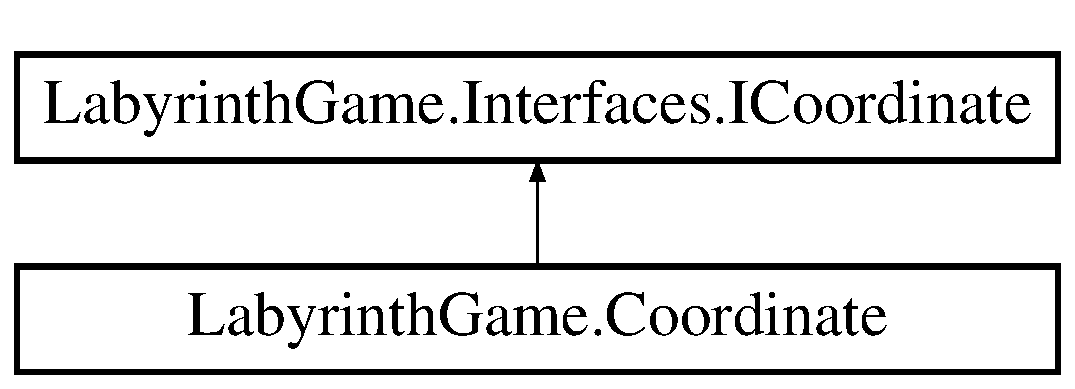
\includegraphics[height=2.000000cm]{class_labyrinth_game_1_1_coordinate}
\end{center}
\end{figure}
\subsection*{Public Member Functions}
\begin{DoxyCompactItemize}
\item 
\hyperlink{class_labyrinth_game_1_1_coordinate_a28179b93dd647822685cd8f94740e91e}{Coordinate} (int row\+Coordinate, int col\+Coordinate)
\begin{DoxyCompactList}\small\item\em Constructor \end{DoxyCompactList}\item 
void \hyperlink{class_labyrinth_game_1_1_coordinate_aa051ffb8f95af1633dafaebd72fbb90e}{Update} (\hyperlink{interface_labyrinth_game_1_1_interfaces_1_1_i_coordinate}{I\+Coordinate} new\+Coordinates)
\begin{DoxyCompactList}\small\item\em Updates coordinates assuming the mark of the given parameters \end{DoxyCompactList}\end{DoxyCompactItemize}
\subsection*{Static Public Member Functions}
\begin{DoxyCompactItemize}
\item 
static \hyperlink{class_labyrinth_game_1_1_coordinate}{Coordinate} \hyperlink{class_labyrinth_game_1_1_coordinate_a3df5678bab1c002539e80b7420edf908}{operator-\/} (\hyperlink{class_labyrinth_game_1_1_coordinate}{Coordinate} first, \hyperlink{class_labyrinth_game_1_1_coordinate}{Coordinate} second)
\begin{DoxyCompactList}\small\item\em Overrides the operation minus \end{DoxyCompactList}\end{DoxyCompactItemize}
\subsection*{Properties}
\begin{DoxyCompactItemize}
\item 
\hypertarget{class_labyrinth_game_1_1_coordinate_a1b5482f9527f8abb145bc866c938820e}{int {\bfseries Col}\hspace{0.3cm}{\ttfamily  \mbox{[}get, set\mbox{]}}}\label{class_labyrinth_game_1_1_coordinate_a1b5482f9527f8abb145bc866c938820e}

\item 
\hypertarget{class_labyrinth_game_1_1_coordinate_abb19a8fa689981d9f3b27d8f3ce5f961}{int {\bfseries Row}\hspace{0.3cm}{\ttfamily  \mbox{[}get, set\mbox{]}}}\label{class_labyrinth_game_1_1_coordinate_abb19a8fa689981d9f3b27d8f3ce5f961}

\end{DoxyCompactItemize}


\subsection{Detailed Description}
The \hyperlink{class_labyrinth_game_1_1_coordinate}{Coordinate} class holds the coordinates which will be used from the other classes(like Player) 



Definition at line 10 of file Coordinate.\+cs.



\subsection{Constructor \& Destructor Documentation}
\hypertarget{class_labyrinth_game_1_1_coordinate_a28179b93dd647822685cd8f94740e91e}{\index{Labyrinth\+Game\+::\+Coordinate@{Labyrinth\+Game\+::\+Coordinate}!Coordinate@{Coordinate}}
\index{Coordinate@{Coordinate}!Labyrinth\+Game\+::\+Coordinate@{Labyrinth\+Game\+::\+Coordinate}}
\subsubsection[{Coordinate}]{\setlength{\rightskip}{0pt plus 5cm}Labyrinth\+Game.\+Coordinate.\+Coordinate (
\begin{DoxyParamCaption}
\item[{int}]{row\+Coordinate, }
\item[{int}]{col\+Coordinate}
\end{DoxyParamCaption}
)}}\label{class_labyrinth_game_1_1_coordinate_a28179b93dd647822685cd8f94740e91e}


Constructor 


\begin{DoxyParams}{Parameters}
{\em row\+Coordinate} & row\\
\hline
{\em col\+Coordinate} & col\\
\hline
\end{DoxyParams}


Definition at line 17 of file Coordinate.\+cs.



\subsection{Member Function Documentation}
\hypertarget{class_labyrinth_game_1_1_coordinate_a3df5678bab1c002539e80b7420edf908}{\index{Labyrinth\+Game\+::\+Coordinate@{Labyrinth\+Game\+::\+Coordinate}!operator-\/@{operator-\/}}
\index{operator-\/@{operator-\/}!Labyrinth\+Game\+::\+Coordinate@{Labyrinth\+Game\+::\+Coordinate}}
\subsubsection[{operator-\/}]{\setlength{\rightskip}{0pt plus 5cm}static {\bf Coordinate} Labyrinth\+Game.\+Coordinate.\+operator-\/ (
\begin{DoxyParamCaption}
\item[{{\bf Coordinate}}]{first, }
\item[{{\bf Coordinate}}]{second}
\end{DoxyParamCaption}
)\hspace{0.3cm}{\ttfamily [static]}}}\label{class_labyrinth_game_1_1_coordinate_a3df5678bab1c002539e80b7420edf908}


Overrides the operation minus 


\begin{DoxyParams}{Parameters}
{\em first} & First inpit parameter of class \hyperlink{class_labyrinth_game_1_1_coordinate}{Coordinate}\\
\hline
{\em second} & Second inpit parameter of class \hyperlink{class_labyrinth_game_1_1_coordinate}{Coordinate}\\
\hline
\end{DoxyParams}
\begin{DoxyReturn}{Returns}
Coordinates
\end{DoxyReturn}


Definition at line 43 of file Coordinate.\+cs.

\hypertarget{class_labyrinth_game_1_1_coordinate_aa051ffb8f95af1633dafaebd72fbb90e}{\index{Labyrinth\+Game\+::\+Coordinate@{Labyrinth\+Game\+::\+Coordinate}!Update@{Update}}
\index{Update@{Update}!Labyrinth\+Game\+::\+Coordinate@{Labyrinth\+Game\+::\+Coordinate}}
\subsubsection[{Update}]{\setlength{\rightskip}{0pt plus 5cm}void Labyrinth\+Game.\+Coordinate.\+Update (
\begin{DoxyParamCaption}
\item[{{\bf I\+Coordinate}}]{new\+Coordinates}
\end{DoxyParamCaption}
)}}\label{class_labyrinth_game_1_1_coordinate_aa051ffb8f95af1633dafaebd72fbb90e}


Updates coordinates assuming the mark of the given parameters 


\begin{DoxyParams}{Parameters}
{\em new\+Coordinates} & Value to change coordinates, that hold row and col\\
\hline
\end{DoxyParams}


Implements \hyperlink{interface_labyrinth_game_1_1_interfaces_1_1_i_coordinate}{Labyrinth\+Game.\+Interfaces.\+I\+Coordinate}.



Definition at line 31 of file Coordinate.\+cs.



The documentation for this class was generated from the following file\+:\begin{DoxyCompactItemize}
\item 
Labyrinth\+Game/Coordinate.\+cs\end{DoxyCompactItemize}

\hypertarget{class_labyrinth_game_test_1_1_coordinate_test}{\section{Labyrinth\+Game\+Test.\+Coordinate\+Test Class Reference}
\label{class_labyrinth_game_test_1_1_coordinate_test}\index{Labyrinth\+Game\+Test.\+Coordinate\+Test@{Labyrinth\+Game\+Test.\+Coordinate\+Test}}
}
\subsection*{Public Member Functions}
\begin{DoxyCompactItemize}
\item 
\hypertarget{class_labyrinth_game_test_1_1_coordinate_test_a0db2897fc8f242a3ba6f155b4374a4e1}{void {\bfseries Row\+Coordinate\+Update\+Test} ()}\label{class_labyrinth_game_test_1_1_coordinate_test_a0db2897fc8f242a3ba6f155b4374a4e1}

\item 
\hypertarget{class_labyrinth_game_test_1_1_coordinate_test_a7c280bfc815c75f41dc8eeafa18284dd}{void {\bfseries Col\+Coordinate\+Update\+Test} ()}\label{class_labyrinth_game_test_1_1_coordinate_test_a7c280bfc815c75f41dc8eeafa18284dd}

\item 
\hypertarget{class_labyrinth_game_test_1_1_coordinate_test_ab639f37f54a20e71512d00cca30ee6ee}{void {\bfseries Coordinate\+Update\+With\+Negative\+Test} ()}\label{class_labyrinth_game_test_1_1_coordinate_test_ab639f37f54a20e71512d00cca30ee6ee}

\item 
\hypertarget{class_labyrinth_game_test_1_1_coordinate_test_a094a760e28bdc165023223ae80410ffc}{void {\bfseries Substraction\+Of\+Coordinates\+Should\+Return\+New\+Coordinate\+Test} ()}\label{class_labyrinth_game_test_1_1_coordinate_test_a094a760e28bdc165023223ae80410ffc}

\item 
\hypertarget{class_labyrinth_game_test_1_1_coordinate_test_a2b36e28c7def15a0ec3bd14877fe410e}{void {\bfseries Substraction\+Of\+Bigger\+Coordinates\+Should\+Return\+New\+Coordinate\+Test} ()}\label{class_labyrinth_game_test_1_1_coordinate_test_a2b36e28c7def15a0ec3bd14877fe410e}

\end{DoxyCompactItemize}


\subsection{Detailed Description}


Definition at line 8 of file Coordinate\+Test.\+cs.



The documentation for this class was generated from the following file\+:\begin{DoxyCompactItemize}
\item 
Labyrinth\+Game\+Test/Coordinate\+Test.\+cs\end{DoxyCompactItemize}

\hypertarget{class_labyrinth_game_1_1_labyrinths_1_1_diamond_labyrinth}{\section{Labyrinth\+Game.\+Labyrinths.\+Diamond\+Labyrinth Class Reference}
\label{class_labyrinth_game_1_1_labyrinths_1_1_diamond_labyrinth}\index{Labyrinth\+Game.\+Labyrinths.\+Diamond\+Labyrinth@{Labyrinth\+Game.\+Labyrinths.\+Diamond\+Labyrinth}}
}


\hyperlink{class_labyrinth_game_1_1_labyrinths_1_1_labyrinth}{Labyrinth} with shape like diamond  


Inheritance diagram for Labyrinth\+Game.\+Labyrinths.\+Diamond\+Labyrinth\+:\begin{figure}[H]
\begin{center}
\leavevmode
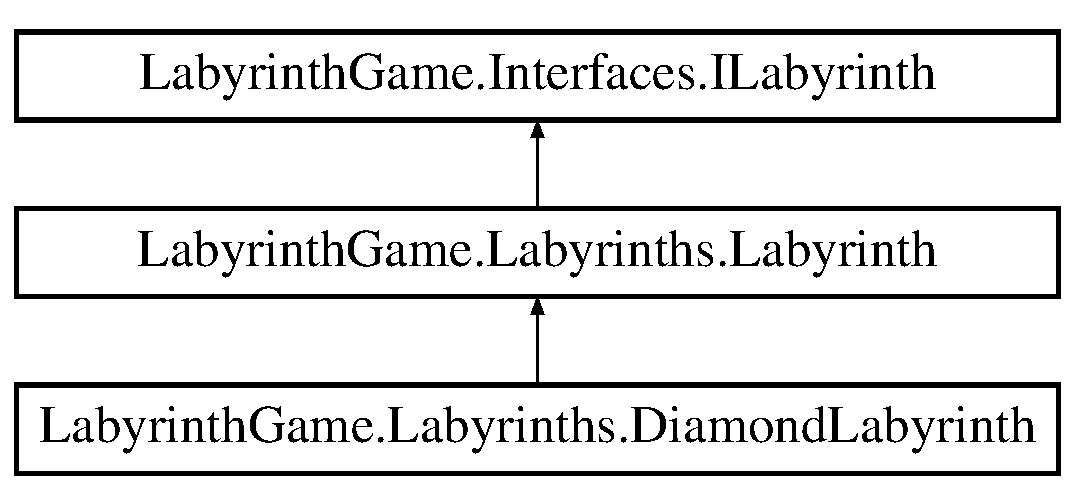
\includegraphics[height=3.000000cm]{class_labyrinth_game_1_1_labyrinths_1_1_diamond_labyrinth}
\end{center}
\end{figure}
\subsection*{Public Member Functions}
\begin{DoxyCompactItemize}
\item 
\hypertarget{class_labyrinth_game_1_1_labyrinths_1_1_diamond_labyrinth_ae4452baf90cdc6f083fcb8c96b007ea8}{{\bfseries Diamond\+Labyrinth} (\hyperlink{interface_labyrinth_game_1_1_interfaces_1_1_i_renderer}{I\+Renderer} renderer)}\label{class_labyrinth_game_1_1_labyrinths_1_1_diamond_labyrinth_ae4452baf90cdc6f083fcb8c96b007ea8}

\item 
override void \hyperlink{class_labyrinth_game_1_1_labyrinths_1_1_diamond_labyrinth_ae110be09830e8a79d733e37d4916edde}{Fill\+Matrix} (\hyperlink{interface_labyrinth_game_1_1_interfaces_1_1_i_random_char_provider}{I\+Random\+Char\+Provider} random\+Char\+Provider)
\begin{DoxyCompactList}\small\item\em The method fills the matrix with symbols forming diamond shape \end{DoxyCompactList}\end{DoxyCompactItemize}
\subsection*{Protected Member Functions}
\begin{DoxyCompactItemize}
\item 
override bool \hyperlink{class_labyrinth_game_1_1_labyrinths_1_1_diamond_labyrinth_a4a99398d9794ae845d0e9139f69465fe}{Is\+Blank\+Space\+Sign} (int row, int col)
\begin{DoxyCompactList}\small\item\em The methods checks if sign is blank space or not \end{DoxyCompactList}\end{DoxyCompactItemize}
\subsection*{Additional Inherited Members}


\subsection{Detailed Description}
\hyperlink{class_labyrinth_game_1_1_labyrinths_1_1_labyrinth}{Labyrinth} with shape like diamond 



Definition at line 9 of file Diamond\+Labyrinth.\+cs.



\subsection{Member Function Documentation}
\hypertarget{class_labyrinth_game_1_1_labyrinths_1_1_diamond_labyrinth_ae110be09830e8a79d733e37d4916edde}{\index{Labyrinth\+Game\+::\+Labyrinths\+::\+Diamond\+Labyrinth@{Labyrinth\+Game\+::\+Labyrinths\+::\+Diamond\+Labyrinth}!Fill\+Matrix@{Fill\+Matrix}}
\index{Fill\+Matrix@{Fill\+Matrix}!Labyrinth\+Game\+::\+Labyrinths\+::\+Diamond\+Labyrinth@{Labyrinth\+Game\+::\+Labyrinths\+::\+Diamond\+Labyrinth}}
\subsubsection[{Fill\+Matrix}]{\setlength{\rightskip}{0pt plus 5cm}override void Labyrinth\+Game.\+Labyrinths.\+Diamond\+Labyrinth.\+Fill\+Matrix (
\begin{DoxyParamCaption}
\item[{{\bf I\+Random\+Char\+Provider}}]{random\+Char\+Provider}
\end{DoxyParamCaption}
)\hspace{0.3cm}{\ttfamily [virtual]}}}\label{class_labyrinth_game_1_1_labyrinths_1_1_diamond_labyrinth_ae110be09830e8a79d733e37d4916edde}


The method fills the matrix with symbols forming diamond shape 



Implements \hyperlink{class_labyrinth_game_1_1_labyrinths_1_1_labyrinth_a13b3599b7157943b1c028b2f0f5df26c}{Labyrinth\+Game.\+Labyrinths.\+Labyrinth}.



Definition at line 26 of file Diamond\+Labyrinth.\+cs.

\hypertarget{class_labyrinth_game_1_1_labyrinths_1_1_diamond_labyrinth_a4a99398d9794ae845d0e9139f69465fe}{\index{Labyrinth\+Game\+::\+Labyrinths\+::\+Diamond\+Labyrinth@{Labyrinth\+Game\+::\+Labyrinths\+::\+Diamond\+Labyrinth}!Is\+Blank\+Space\+Sign@{Is\+Blank\+Space\+Sign}}
\index{Is\+Blank\+Space\+Sign@{Is\+Blank\+Space\+Sign}!Labyrinth\+Game\+::\+Labyrinths\+::\+Diamond\+Labyrinth@{Labyrinth\+Game\+::\+Labyrinths\+::\+Diamond\+Labyrinth}}
\subsubsection[{Is\+Blank\+Space\+Sign}]{\setlength{\rightskip}{0pt plus 5cm}override bool Labyrinth\+Game.\+Labyrinths.\+Diamond\+Labyrinth.\+Is\+Blank\+Space\+Sign (
\begin{DoxyParamCaption}
\item[{int}]{row, }
\item[{int}]{col}
\end{DoxyParamCaption}
)\hspace{0.3cm}{\ttfamily [protected]}, {\ttfamily [virtual]}}}\label{class_labyrinth_game_1_1_labyrinths_1_1_diamond_labyrinth_a4a99398d9794ae845d0e9139f69465fe}


The methods checks if sign is blank space or not 


\begin{DoxyParams}{Parameters}
{\em row} & The row we want to check\\
\hline
{\em col} & The column we want to check\\
\hline
\end{DoxyParams}
\begin{DoxyReturn}{Returns}
Returns boolean value -\/ true if it is blank space and false id it is not
\end{DoxyReturn}


Implements \hyperlink{class_labyrinth_game_1_1_labyrinths_1_1_labyrinth_a1f35ce958322025715acf77852f112fa}{Labyrinth\+Game.\+Labyrinths.\+Labyrinth}.



Definition at line 52 of file Diamond\+Labyrinth.\+cs.



The documentation for this class was generated from the following file\+:\begin{DoxyCompactItemize}
\item 
Labyrinth\+Game/\+Labyrinths/Diamond\+Labyrinth.\+cs\end{DoxyCompactItemize}

\hypertarget{class_labyrinth_game_test_1_1_labyrinths_test_1_1_diamond_labyrinth_test}{\section{Labyrinth\+Game\+Test.\+Labyrinths\+Test.\+Diamond\+Labyrinth\+Test Class Reference}
\label{class_labyrinth_game_test_1_1_labyrinths_test_1_1_diamond_labyrinth_test}\index{Labyrinth\+Game\+Test.\+Labyrinths\+Test.\+Diamond\+Labyrinth\+Test@{Labyrinth\+Game\+Test.\+Labyrinths\+Test.\+Diamond\+Labyrinth\+Test}}
}
\subsection*{Public Member Functions}
\begin{DoxyCompactItemize}
\item 
\hypertarget{class_labyrinth_game_test_1_1_labyrinths_test_1_1_diamond_labyrinth_test_a5380f682a09e0486b59dd35a1d1f315b}{void {\bfseries Is\+Diamnod\+Labyrinth\+Matrix\+Filled} ()}\label{class_labyrinth_game_test_1_1_labyrinths_test_1_1_diamond_labyrinth_test_a5380f682a09e0486b59dd35a1d1f315b}

\end{DoxyCompactItemize}


\subsection{Detailed Description}


Definition at line 11 of file Diamond\+Labyrinth\+Test.\+cs.



The documentation for this class was generated from the following file\+:\begin{DoxyCompactItemize}
\item 
Labyrinth\+Game\+Test/\+Labyrinths\+Test/Diamond\+Labyrinth\+Test.\+cs\end{DoxyCompactItemize}

\hypertarget{class_labyrinth_game_demo_1_1_game_demo}{\section{Labyrinth\+Game\+Demo.\+Game\+Demo Class Reference}
\label{class_labyrinth_game_demo_1_1_game_demo}\index{Labyrinth\+Game\+Demo.\+Game\+Demo@{Labyrinth\+Game\+Demo.\+Game\+Demo}}
}


Game demo class  




\subsection{Detailed Description}
Game demo class 



Definition at line 8 of file Game\+Demo.\+cs.



The documentation for this class was generated from the following file\+:\begin{DoxyCompactItemize}
\item 
Labyrinth\+Game\+Demo/Game\+Demo.\+cs\end{DoxyCompactItemize}

\hypertarget{class_labyrinth_game_1_1_labyrinths_1_1_hexagonal_labyrinth}{\section{Labyrinth\+Game.\+Labyrinths.\+Hexagonal\+Labyrinth Class Reference}
\label{class_labyrinth_game_1_1_labyrinths_1_1_hexagonal_labyrinth}\index{Labyrinth\+Game.\+Labyrinths.\+Hexagonal\+Labyrinth@{Labyrinth\+Game.\+Labyrinths.\+Hexagonal\+Labyrinth}}
}


\hyperlink{class_labyrinth_game_1_1_labyrinths_1_1_labyrinth}{Labyrinth} with shape like hexagon  


Inheritance diagram for Labyrinth\+Game.\+Labyrinths.\+Hexagonal\+Labyrinth\+:\begin{figure}[H]
\begin{center}
\leavevmode
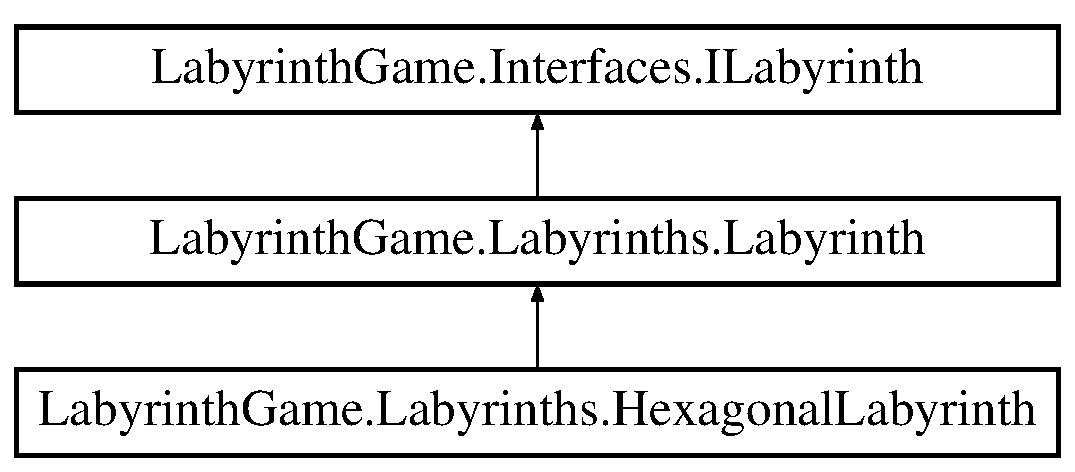
\includegraphics[height=3.000000cm]{class_labyrinth_game_1_1_labyrinths_1_1_hexagonal_labyrinth}
\end{center}
\end{figure}
\subsection*{Public Member Functions}
\begin{DoxyCompactItemize}
\item 
\hypertarget{class_labyrinth_game_1_1_labyrinths_1_1_hexagonal_labyrinth_ac3f6de2b1b38148925b98f235d43767d}{{\bfseries Hexagonal\+Labyrinth} (\hyperlink{interface_labyrinth_game_1_1_interfaces_1_1_i_renderer}{I\+Renderer} renderer)}\label{class_labyrinth_game_1_1_labyrinths_1_1_hexagonal_labyrinth_ac3f6de2b1b38148925b98f235d43767d}

\item 
override void \hyperlink{class_labyrinth_game_1_1_labyrinths_1_1_hexagonal_labyrinth_af1d2c0c78d13dd85c421ded3dae0a062}{Fill\+Matrix} (\hyperlink{interface_labyrinth_game_1_1_interfaces_1_1_i_random_char_provider}{I\+Random\+Char\+Provider} random\+Char\+Provider)
\begin{DoxyCompactList}\small\item\em The method fills the matrix with symbols forming hexagon shape \end{DoxyCompactList}\end{DoxyCompactItemize}
\subsection*{Protected Member Functions}
\begin{DoxyCompactItemize}
\item 
override bool \hyperlink{class_labyrinth_game_1_1_labyrinths_1_1_hexagonal_labyrinth_a88db5627f18a0a6ebd2b7da78388a925}{Is\+Blank\+Space\+Sign} (int row, int col)
\begin{DoxyCompactList}\small\item\em The methods checks if sign is blank space or not \end{DoxyCompactList}\end{DoxyCompactItemize}
\subsection*{Additional Inherited Members}


\subsection{Detailed Description}
\hyperlink{class_labyrinth_game_1_1_labyrinths_1_1_labyrinth}{Labyrinth} with shape like hexagon 



Definition at line 9 of file Hexagonal\+Labyrinth.\+cs.



\subsection{Member Function Documentation}
\hypertarget{class_labyrinth_game_1_1_labyrinths_1_1_hexagonal_labyrinth_af1d2c0c78d13dd85c421ded3dae0a062}{\index{Labyrinth\+Game\+::\+Labyrinths\+::\+Hexagonal\+Labyrinth@{Labyrinth\+Game\+::\+Labyrinths\+::\+Hexagonal\+Labyrinth}!Fill\+Matrix@{Fill\+Matrix}}
\index{Fill\+Matrix@{Fill\+Matrix}!Labyrinth\+Game\+::\+Labyrinths\+::\+Hexagonal\+Labyrinth@{Labyrinth\+Game\+::\+Labyrinths\+::\+Hexagonal\+Labyrinth}}
\subsubsection[{Fill\+Matrix}]{\setlength{\rightskip}{0pt plus 5cm}override void Labyrinth\+Game.\+Labyrinths.\+Hexagonal\+Labyrinth.\+Fill\+Matrix (
\begin{DoxyParamCaption}
\item[{{\bf I\+Random\+Char\+Provider}}]{random\+Char\+Provider}
\end{DoxyParamCaption}
)\hspace{0.3cm}{\ttfamily [virtual]}}}\label{class_labyrinth_game_1_1_labyrinths_1_1_hexagonal_labyrinth_af1d2c0c78d13dd85c421ded3dae0a062}


The method fills the matrix with symbols forming hexagon shape 



Implements \hyperlink{class_labyrinth_game_1_1_labyrinths_1_1_labyrinth_a13b3599b7157943b1c028b2f0f5df26c}{Labyrinth\+Game.\+Labyrinths.\+Labyrinth}.



Definition at line 27 of file Hexagonal\+Labyrinth.\+cs.

\hypertarget{class_labyrinth_game_1_1_labyrinths_1_1_hexagonal_labyrinth_a88db5627f18a0a6ebd2b7da78388a925}{\index{Labyrinth\+Game\+::\+Labyrinths\+::\+Hexagonal\+Labyrinth@{Labyrinth\+Game\+::\+Labyrinths\+::\+Hexagonal\+Labyrinth}!Is\+Blank\+Space\+Sign@{Is\+Blank\+Space\+Sign}}
\index{Is\+Blank\+Space\+Sign@{Is\+Blank\+Space\+Sign}!Labyrinth\+Game\+::\+Labyrinths\+::\+Hexagonal\+Labyrinth@{Labyrinth\+Game\+::\+Labyrinths\+::\+Hexagonal\+Labyrinth}}
\subsubsection[{Is\+Blank\+Space\+Sign}]{\setlength{\rightskip}{0pt plus 5cm}override bool Labyrinth\+Game.\+Labyrinths.\+Hexagonal\+Labyrinth.\+Is\+Blank\+Space\+Sign (
\begin{DoxyParamCaption}
\item[{int}]{row, }
\item[{int}]{col}
\end{DoxyParamCaption}
)\hspace{0.3cm}{\ttfamily [protected]}, {\ttfamily [virtual]}}}\label{class_labyrinth_game_1_1_labyrinths_1_1_hexagonal_labyrinth_a88db5627f18a0a6ebd2b7da78388a925}


The methods checks if sign is blank space or not 


\begin{DoxyParams}{Parameters}
{\em row} & The row we want to check\\
\hline
{\em col} & The column we want to check\\
\hline
\end{DoxyParams}
\begin{DoxyReturn}{Returns}
Returns boolean value -\/ true if it is blank space and false id it is not
\end{DoxyReturn}


Implements \hyperlink{class_labyrinth_game_1_1_labyrinths_1_1_labyrinth_a1f35ce958322025715acf77852f112fa}{Labyrinth\+Game.\+Labyrinths.\+Labyrinth}.



Definition at line 53 of file Hexagonal\+Labyrinth.\+cs.



The documentation for this class was generated from the following file\+:\begin{DoxyCompactItemize}
\item 
Labyrinth\+Game/\+Labyrinths/Hexagonal\+Labyrinth.\+cs\end{DoxyCompactItemize}

\hypertarget{class_labyrinth_game_test_1_1_labyrinths_test_1_1_hexagonal_labyrinth_test}{\section{Labyrinth\+Game\+Test.\+Labyrinths\+Test.\+Hexagonal\+Labyrinth\+Test Class Reference}
\label{class_labyrinth_game_test_1_1_labyrinths_test_1_1_hexagonal_labyrinth_test}\index{Labyrinth\+Game\+Test.\+Labyrinths\+Test.\+Hexagonal\+Labyrinth\+Test@{Labyrinth\+Game\+Test.\+Labyrinths\+Test.\+Hexagonal\+Labyrinth\+Test}}
}
\subsection*{Public Member Functions}
\begin{DoxyCompactItemize}
\item 
\hypertarget{class_labyrinth_game_test_1_1_labyrinths_test_1_1_hexagonal_labyrinth_test_aeb7ab8e1dcd18d0e9a9fa4c2265d168e}{void {\bfseries Is\+Hexagonal\+Labyrinth\+Matrix\+Filled} ()}\label{class_labyrinth_game_test_1_1_labyrinths_test_1_1_hexagonal_labyrinth_test_aeb7ab8e1dcd18d0e9a9fa4c2265d168e}

\end{DoxyCompactItemize}


\subsection{Detailed Description}


Definition at line 11 of file Hexagonal\+Labyrinth\+Test.\+cs.



The documentation for this class was generated from the following file\+:\begin{DoxyCompactItemize}
\item 
Labyrinth\+Game\+Test/\+Labyrinths\+Test/Hexagonal\+Labyrinth\+Test.\+cs\end{DoxyCompactItemize}

\hypertarget{interface_labyrinth_game_1_1_interfaces_1_1_i_coordinate}{\section{Labyrinth\+Game.\+Interfaces.\+I\+Coordinate Interface Reference}
\label{interface_labyrinth_game_1_1_interfaces_1_1_i_coordinate}\index{Labyrinth\+Game.\+Interfaces.\+I\+Coordinate@{Labyrinth\+Game.\+Interfaces.\+I\+Coordinate}}
}


Interface which is inherited by the \hyperlink{class_labyrinth_game_1_1_coordinate}{Coordinate} class  


Inheritance diagram for Labyrinth\+Game.\+Interfaces.\+I\+Coordinate\+:\begin{figure}[H]
\begin{center}
\leavevmode
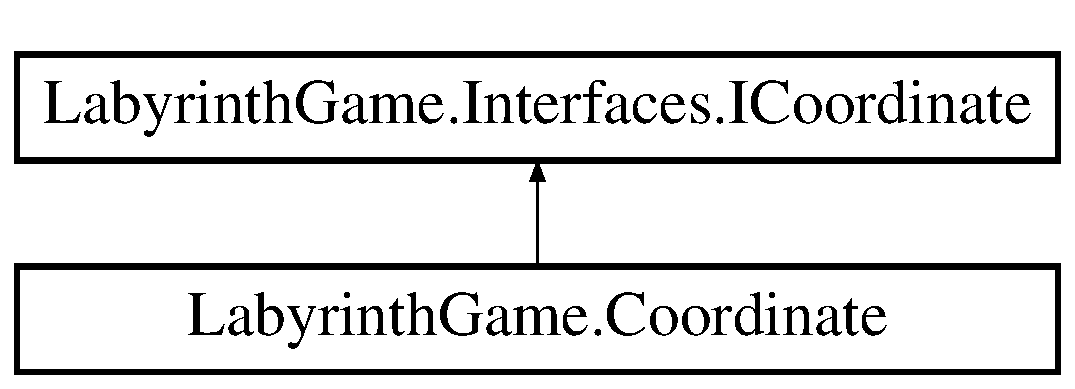
\includegraphics[height=2.000000cm]{interface_labyrinth_game_1_1_interfaces_1_1_i_coordinate}
\end{center}
\end{figure}
\subsection*{Public Member Functions}
\begin{DoxyCompactItemize}
\item 
\hypertarget{interface_labyrinth_game_1_1_interfaces_1_1_i_coordinate_ac898b2b5a6f3d7ba942d54c3815c97f8}{void {\bfseries Update} (\hyperlink{interface_labyrinth_game_1_1_interfaces_1_1_i_coordinate}{I\+Coordinate} new\+Coordinates)}\label{interface_labyrinth_game_1_1_interfaces_1_1_i_coordinate_ac898b2b5a6f3d7ba942d54c3815c97f8}

\end{DoxyCompactItemize}
\subsection*{Properties}
\begin{DoxyCompactItemize}
\item 
\hypertarget{interface_labyrinth_game_1_1_interfaces_1_1_i_coordinate_ae21b7a7e0ba1b797254b38088f76693a}{int {\bfseries Col}\hspace{0.3cm}{\ttfamily  \mbox{[}get\mbox{]}}}\label{interface_labyrinth_game_1_1_interfaces_1_1_i_coordinate_ae21b7a7e0ba1b797254b38088f76693a}

\item 
\hypertarget{interface_labyrinth_game_1_1_interfaces_1_1_i_coordinate_aa75fdf8b6ec615d943533ba6b360a89c}{int {\bfseries Row}\hspace{0.3cm}{\ttfamily  \mbox{[}get\mbox{]}}}\label{interface_labyrinth_game_1_1_interfaces_1_1_i_coordinate_aa75fdf8b6ec615d943533ba6b360a89c}

\end{DoxyCompactItemize}


\subsection{Detailed Description}
Interface which is inherited by the \hyperlink{class_labyrinth_game_1_1_coordinate}{Coordinate} class 



Definition at line 9 of file I\+Coordinate.\+cs.



The documentation for this interface was generated from the following file\+:\begin{DoxyCompactItemize}
\item 
Labyrinth\+Game/\+Interfaces/I\+Coordinate.\+cs\end{DoxyCompactItemize}

\hypertarget{interface_labyrinth_game_1_1_interfaces_1_1_i_labyrinth}{\section{Labyrinth\+Game.\+Interfaces.\+I\+Labyrinth Interface Reference}
\label{interface_labyrinth_game_1_1_interfaces_1_1_i_labyrinth}\index{Labyrinth\+Game.\+Interfaces.\+I\+Labyrinth@{Labyrinth\+Game.\+Interfaces.\+I\+Labyrinth}}
}


Interface which is inherited by the Labyrinth class  


Inheritance diagram for Labyrinth\+Game.\+Interfaces.\+I\+Labyrinth\+:\begin{figure}[H]
\begin{center}
\leavevmode
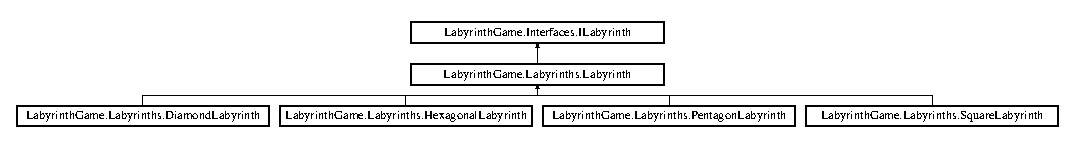
\includegraphics[height=1.473684cm]{interface_labyrinth_game_1_1_interfaces_1_1_i_labyrinth}
\end{center}
\end{figure}
\subsection*{Public Member Functions}
\begin{DoxyCompactItemize}
\item 
\hypertarget{interface_labyrinth_game_1_1_interfaces_1_1_i_labyrinth_a949a13949711b621a487d3efcd37b0eb}{void {\bfseries Fill\+Matrix} (\hyperlink{interface_labyrinth_game_1_1_interfaces_1_1_i_random_char_provider}{I\+Random\+Char\+Provider} random\+Char\+Provider)}\label{interface_labyrinth_game_1_1_interfaces_1_1_i_labyrinth_a949a13949711b621a487d3efcd37b0eb}

\item 
\hypertarget{interface_labyrinth_game_1_1_interfaces_1_1_i_labyrinth_a921c8376d2a59e784f1e95b355722b0a}{void {\bfseries Change\+Symbol} (\hyperlink{interface_labyrinth_game_1_1_interfaces_1_1_i_coordinate}{I\+Coordinate} coordinates, char new\+Symbol)}\label{interface_labyrinth_game_1_1_interfaces_1_1_i_labyrinth_a921c8376d2a59e784f1e95b355722b0a}

\end{DoxyCompactItemize}
\subsection*{Properties}
\begin{DoxyCompactItemize}
\item 
\hypertarget{interface_labyrinth_game_1_1_interfaces_1_1_i_labyrinth_af48030cf8898560b662ac445edc11acd}{char\mbox{[},\mbox{]} {\bfseries Matrix}\hspace{0.3cm}{\ttfamily  \mbox{[}get\mbox{]}}}\label{interface_labyrinth_game_1_1_interfaces_1_1_i_labyrinth_af48030cf8898560b662ac445edc11acd}

\end{DoxyCompactItemize}


\subsection{Detailed Description}
Interface which is inherited by the Labyrinth class 



Definition at line 6 of file I\+Labyrinth.\+cs.



The documentation for this interface was generated from the following file\+:\begin{DoxyCompactItemize}
\item 
Labyrinth\+Game/\+Interfaces/I\+Labyrinth.\+cs\end{DoxyCompactItemize}

\hypertarget{interface_labyrinth_game_1_1_interfaces_1_1_i_labyrinth_creator}{\section{Labyrinth\+Game.\+Interfaces.\+I\+Labyrinth\+Creator Interface Reference}
\label{interface_labyrinth_game_1_1_interfaces_1_1_i_labyrinth_creator}\index{Labyrinth\+Game.\+Interfaces.\+I\+Labyrinth\+Creator@{Labyrinth\+Game.\+Interfaces.\+I\+Labyrinth\+Creator}}
}


Main logic for creating labyrinth.  


Inheritance diagram for Labyrinth\+Game.\+Interfaces.\+I\+Labyrinth\+Creator\+:\begin{figure}[H]
\begin{center}
\leavevmode
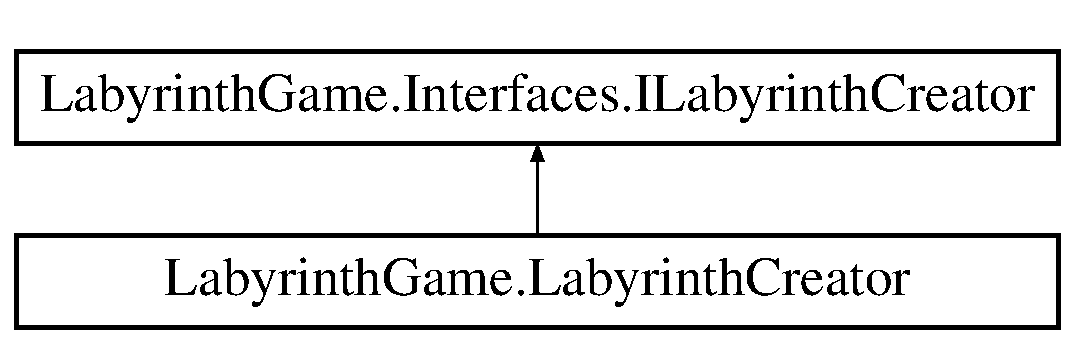
\includegraphics[height=2.000000cm]{interface_labyrinth_game_1_1_interfaces_1_1_i_labyrinth_creator}
\end{center}
\end{figure}
\subsection*{Public Member Functions}
\begin{DoxyCompactItemize}
\item 
\hypertarget{interface_labyrinth_game_1_1_interfaces_1_1_i_labyrinth_creator_a334f9f215d40d3854ad00f36645c347c}{\hyperlink{interface_labyrinth_game_1_1_interfaces_1_1_i_labyrinth}{I\+Labyrinth} {\bfseries Create} (string type\+Labyrinth)}\label{interface_labyrinth_game_1_1_interfaces_1_1_i_labyrinth_creator_a334f9f215d40d3854ad00f36645c347c}

\end{DoxyCompactItemize}


\subsection{Detailed Description}
Main logic for creating labyrinth. 



Definition at line 6 of file I\+Labyrinth\+Creator.\+cs.



The documentation for this interface was generated from the following file\+:\begin{DoxyCompactItemize}
\item 
Labyrinth\+Game/\+Interfaces/I\+Labyrinth\+Creator.\+cs\end{DoxyCompactItemize}

\hypertarget{interface_labyrinth_game_1_1_interfaces_1_1_i_labyrinth_engine}{\section{Labyrinth\+Game.\+Interfaces.\+I\+Labyrinth\+Engine Interface Reference}
\label{interface_labyrinth_game_1_1_interfaces_1_1_i_labyrinth_engine}\index{Labyrinth\+Game.\+Interfaces.\+I\+Labyrinth\+Engine@{Labyrinth\+Game.\+Interfaces.\+I\+Labyrinth\+Engine}}
}


Interface which is inherited by the \hyperlink{class_labyrinth_game_1_1_labyrinth_engine}{Labyrinth\+Engine} class  


Inheritance diagram for Labyrinth\+Game.\+Interfaces.\+I\+Labyrinth\+Engine\+:\begin{figure}[H]
\begin{center}
\leavevmode
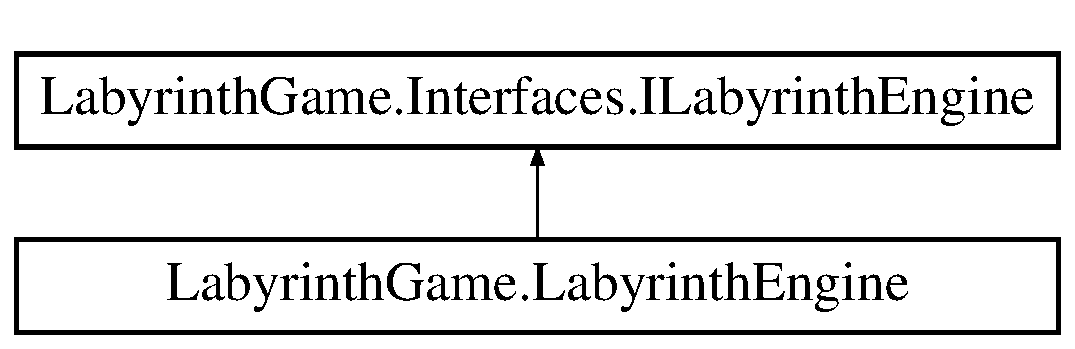
\includegraphics[height=2.000000cm]{interface_labyrinth_game_1_1_interfaces_1_1_i_labyrinth_engine}
\end{center}
\end{figure}
\subsection*{Public Member Functions}
\begin{DoxyCompactItemize}
\item 
\hypertarget{interface_labyrinth_game_1_1_interfaces_1_1_i_labyrinth_engine_a1996d2d63b77bd1ba178ef03da5aa1bc}{void {\bfseries Start} ()}\label{interface_labyrinth_game_1_1_interfaces_1_1_i_labyrinth_engine_a1996d2d63b77bd1ba178ef03da5aa1bc}

\end{DoxyCompactItemize}


\subsection{Detailed Description}
Interface which is inherited by the \hyperlink{class_labyrinth_game_1_1_labyrinth_engine}{Labyrinth\+Engine} class 



Definition at line 9 of file I\+Labyrinth\+Engine.\+cs.



The documentation for this interface was generated from the following file\+:\begin{DoxyCompactItemize}
\item 
Labyrinth\+Game/\+Interfaces/I\+Labyrinth\+Engine.\+cs\end{DoxyCompactItemize}

\hypertarget{interface_labyrinth_game_1_1_interfaces_1_1_i_menu}{\section{Labyrinth\+Game.\+Interfaces.\+I\+Menu Interface Reference}
\label{interface_labyrinth_game_1_1_interfaces_1_1_i_menu}\index{Labyrinth\+Game.\+Interfaces.\+I\+Menu@{Labyrinth\+Game.\+Interfaces.\+I\+Menu}}
}


Interface which is inherited by the \hyperlink{class_labyrinth_game_1_1_menu}{Menu} class  


Inheritance diagram for Labyrinth\+Game.\+Interfaces.\+I\+Menu\+:\begin{figure}[H]
\begin{center}
\leavevmode
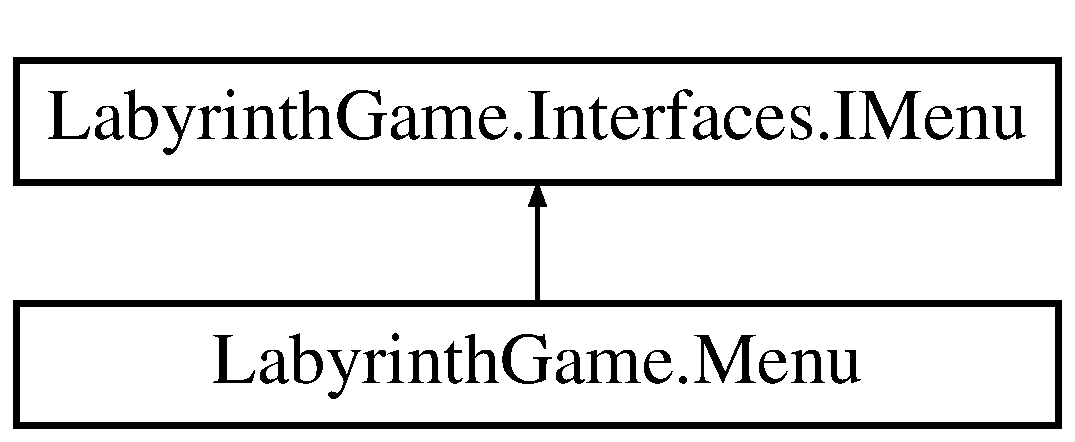
\includegraphics[height=2.000000cm]{interface_labyrinth_game_1_1_interfaces_1_1_i_menu}
\end{center}
\end{figure}
\subsection*{Public Member Functions}
\begin{DoxyCompactItemize}
\item 
\hypertarget{interface_labyrinth_game_1_1_interfaces_1_1_i_menu_a603775084a102a188f3daa186c66d4ef}{string {\bfseries Get\+User\+Choice} ()}\label{interface_labyrinth_game_1_1_interfaces_1_1_i_menu_a603775084a102a188f3daa186c66d4ef}

\item 
\hypertarget{interface_labyrinth_game_1_1_interfaces_1_1_i_menu_ad4f4a4a4c1c42c2b393bcd3a1e0cf6a3}{string {\bfseries Get\+Labyrinth\+Type\+From\+User} ()}\label{interface_labyrinth_game_1_1_interfaces_1_1_i_menu_ad4f4a4a4c1c42c2b393bcd3a1e0cf6a3}

\item 
\hypertarget{interface_labyrinth_game_1_1_interfaces_1_1_i_menu_ab30cce6440656cd63ab3e614c9450859}{void {\bfseries Main\+Menu} ()}\label{interface_labyrinth_game_1_1_interfaces_1_1_i_menu_ab30cce6440656cd63ab3e614c9450859}

\item 
\hypertarget{interface_labyrinth_game_1_1_interfaces_1_1_i_menu_a5c6b9028f1c5e6b0f0c59278bf877cab}{void {\bfseries Menu\+During\+Play} ()}\label{interface_labyrinth_game_1_1_interfaces_1_1_i_menu_a5c6b9028f1c5e6b0f0c59278bf877cab}

\end{DoxyCompactItemize}


\subsection{Detailed Description}
Interface which is inherited by the \hyperlink{class_labyrinth_game_1_1_menu}{Menu} class 



Definition at line 9 of file I\+Menu.\+cs.



The documentation for this interface was generated from the following file\+:\begin{DoxyCompactItemize}
\item 
Labyrinth\+Game/\+Interfaces/I\+Menu.\+cs\end{DoxyCompactItemize}

\hypertarget{interface_labyrinth_game_1_1_interfaces_1_1_i_player}{\section{Labyrinth\+Game.\+Interfaces.\+I\+Player Interface Reference}
\label{interface_labyrinth_game_1_1_interfaces_1_1_i_player}\index{Labyrinth\+Game.\+Interfaces.\+I\+Player@{Labyrinth\+Game.\+Interfaces.\+I\+Player}}
}


Interface which is inherited by the \hyperlink{class_labyrinth_game_1_1_player}{Player} class  


Inheritance diagram for Labyrinth\+Game.\+Interfaces.\+I\+Player\+:\begin{figure}[H]
\begin{center}
\leavevmode
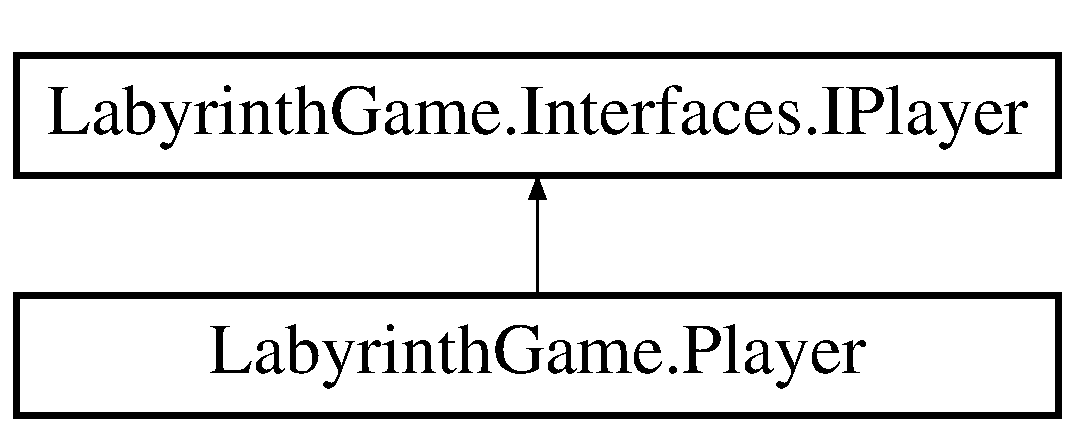
\includegraphics[height=2.000000cm]{interface_labyrinth_game_1_1_interfaces_1_1_i_player}
\end{center}
\end{figure}
\subsection*{Public Member Functions}
\begin{DoxyCompactItemize}
\item 
\hypertarget{interface_labyrinth_game_1_1_interfaces_1_1_i_player_ac5434e0343d317b160fda2624bac1fb5}{void {\bfseries Update\+Points} ()}\label{interface_labyrinth_game_1_1_interfaces_1_1_i_player_ac5434e0343d317b160fda2624bac1fb5}

\item 
\hypertarget{interface_labyrinth_game_1_1_interfaces_1_1_i_player_a90eec2568366b814e522982d2dbb4c8d}{void {\bfseries Update\+Position} (\hyperlink{interface_labyrinth_game_1_1_interfaces_1_1_i_coordinate}{I\+Coordinate} new\+Coordinates)}\label{interface_labyrinth_game_1_1_interfaces_1_1_i_player_a90eec2568366b814e522982d2dbb4c8d}

\item 
\hypertarget{interface_labyrinth_game_1_1_interfaces_1_1_i_player_a95f66bba326c5034c5b37b89d93a2502}{void {\bfseries Show\+Player} (\hyperlink{interface_labyrinth_game_1_1_interfaces_1_1_i_labyrinth}{I\+Labyrinth} labyrinth)}\label{interface_labyrinth_game_1_1_interfaces_1_1_i_player_a95f66bba326c5034c5b37b89d93a2502}

\item 
\hypertarget{interface_labyrinth_game_1_1_interfaces_1_1_i_player_a3879574fee6f751f8b967697cb07b21c}{void {\bfseries Remove\+Player} (\hyperlink{interface_labyrinth_game_1_1_interfaces_1_1_i_labyrinth}{I\+Labyrinth} labyrinth)}\label{interface_labyrinth_game_1_1_interfaces_1_1_i_player_a3879574fee6f751f8b967697cb07b21c}

\end{DoxyCompactItemize}
\subsection*{Properties}
\begin{DoxyCompactItemize}
\item 
\hypertarget{interface_labyrinth_game_1_1_interfaces_1_1_i_player_ada91c3312fd708c5c66da510529a5602}{string {\bfseries Name}\hspace{0.3cm}{\ttfamily  \mbox{[}get, set\mbox{]}}}\label{interface_labyrinth_game_1_1_interfaces_1_1_i_player_ada91c3312fd708c5c66da510529a5602}

\item 
\hypertarget{interface_labyrinth_game_1_1_interfaces_1_1_i_player_aaa644f1f84177bdf8760bef94f9c8467}{int {\bfseries Points}\hspace{0.3cm}{\ttfamily  \mbox{[}get\mbox{]}}}\label{interface_labyrinth_game_1_1_interfaces_1_1_i_player_aaa644f1f84177bdf8760bef94f9c8467}

\item 
\hypertarget{interface_labyrinth_game_1_1_interfaces_1_1_i_player_a78df99d940e4e8cb40215ebcc2319809}{\hyperlink{class_labyrinth_game_1_1_coordinate}{Coordinate} {\bfseries Coordinates}\hspace{0.3cm}{\ttfamily  \mbox{[}get, set\mbox{]}}}\label{interface_labyrinth_game_1_1_interfaces_1_1_i_player_a78df99d940e4e8cb40215ebcc2319809}

\end{DoxyCompactItemize}


\subsection{Detailed Description}
Interface which is inherited by the \hyperlink{class_labyrinth_game_1_1_player}{Player} class 



Definition at line 10 of file I\+Player.\+cs.



The documentation for this interface was generated from the following file\+:\begin{DoxyCompactItemize}
\item 
Labyrinth\+Game/\+Interfaces/I\+Player.\+cs\end{DoxyCompactItemize}

\hypertarget{interface_labyrinth_game_1_1_interfaces_1_1_i_random_char_provider}{\section{Labyrinth\+Game.\+Interfaces.\+I\+Random\+Char\+Provider Interface Reference}
\label{interface_labyrinth_game_1_1_interfaces_1_1_i_random_char_provider}\index{Labyrinth\+Game.\+Interfaces.\+I\+Random\+Char\+Provider@{Labyrinth\+Game.\+Interfaces.\+I\+Random\+Char\+Provider}}
}
Inheritance diagram for Labyrinth\+Game.\+Interfaces.\+I\+Random\+Char\+Provider\+:\begin{figure}[H]
\begin{center}
\leavevmode
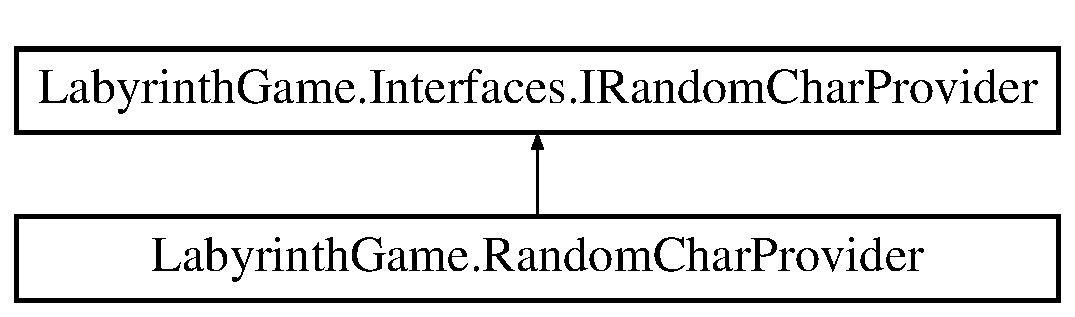
\includegraphics[height=2.000000cm]{interface_labyrinth_game_1_1_interfaces_1_1_i_random_char_provider}
\end{center}
\end{figure}
\subsection*{Public Member Functions}
\begin{DoxyCompactItemize}
\item 
\hypertarget{interface_labyrinth_game_1_1_interfaces_1_1_i_random_char_provider_a05c954dd2de0fd0fc1c7ad10c8d82529}{char {\bfseries Get\+Random\+Symbol} (int chance)}\label{interface_labyrinth_game_1_1_interfaces_1_1_i_random_char_provider_a05c954dd2de0fd0fc1c7ad10c8d82529}

\end{DoxyCompactItemize}


\subsection{Detailed Description}


Definition at line 3 of file I\+Random\+Char\+Provider.\+cs.



The documentation for this interface was generated from the following file\+:\begin{DoxyCompactItemize}
\item 
Labyrinth\+Game/\+Interfaces/I\+Random\+Char\+Provider.\+cs\end{DoxyCompactItemize}

\hypertarget{interface_labyrinth_game_1_1_interfaces_1_1_i_renderer}{\section{Labyrinth\+Game.\+Interfaces.\+I\+Renderer Interface Reference}
\label{interface_labyrinth_game_1_1_interfaces_1_1_i_renderer}\index{Labyrinth\+Game.\+Interfaces.\+I\+Renderer@{Labyrinth\+Game.\+Interfaces.\+I\+Renderer}}
}


Interface that gives the view engine logic, is inherited by the Labyrinth class  


Inheritance diagram for Labyrinth\+Game.\+Interfaces.\+I\+Renderer\+:\begin{figure}[H]
\begin{center}
\leavevmode
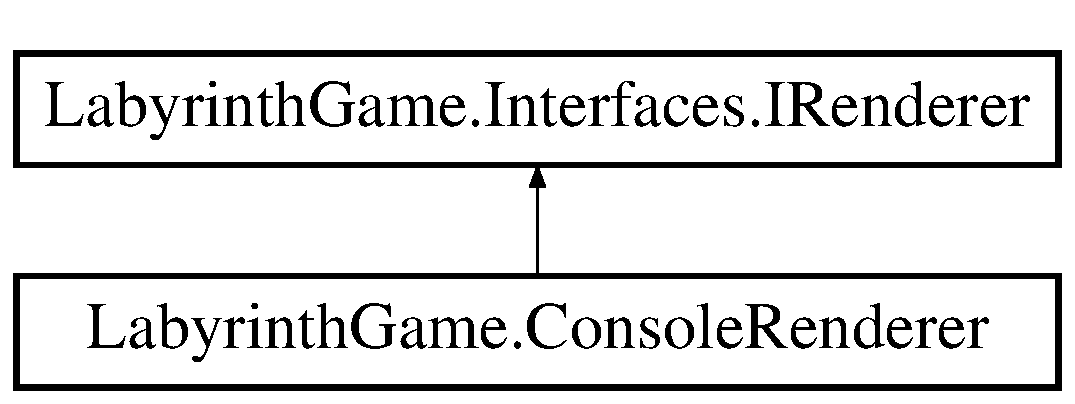
\includegraphics[height=2.000000cm]{interface_labyrinth_game_1_1_interfaces_1_1_i_renderer}
\end{center}
\end{figure}
\subsection*{Public Member Functions}
\begin{DoxyCompactItemize}
\item 
\hypertarget{interface_labyrinth_game_1_1_interfaces_1_1_i_renderer_a6683ba42661c769819043f3c48934e55}{void {\bfseries Render} (\hyperlink{interface_labyrinth_game_1_1_interfaces_1_1_i_labyrinth}{I\+Labyrinth} labyrinth)}\label{interface_labyrinth_game_1_1_interfaces_1_1_i_renderer_a6683ba42661c769819043f3c48934e55}

\end{DoxyCompactItemize}


\subsection{Detailed Description}
Interface that gives the view engine logic, is inherited by the Labyrinth class 



Definition at line 9 of file I\+Renderer.\+cs.



The documentation for this interface was generated from the following file\+:\begin{DoxyCompactItemize}
\item 
Labyrinth\+Game/\+Interfaces/I\+Renderer.\+cs\end{DoxyCompactItemize}

\hypertarget{interface_labyrinth_game_1_1_interfaces_1_1_i_score}{\section{Labyrinth\+Game.\+Interfaces.\+I\+Score Interface Reference}
\label{interface_labyrinth_game_1_1_interfaces_1_1_i_score}\index{Labyrinth\+Game.\+Interfaces.\+I\+Score@{Labyrinth\+Game.\+Interfaces.\+I\+Score}}
}


Interface which is inherited by the \hyperlink{class_labyrinth_game_1_1_score}{Score} class  


Inheritance diagram for Labyrinth\+Game.\+Interfaces.\+I\+Score\+:\begin{figure}[H]
\begin{center}
\leavevmode
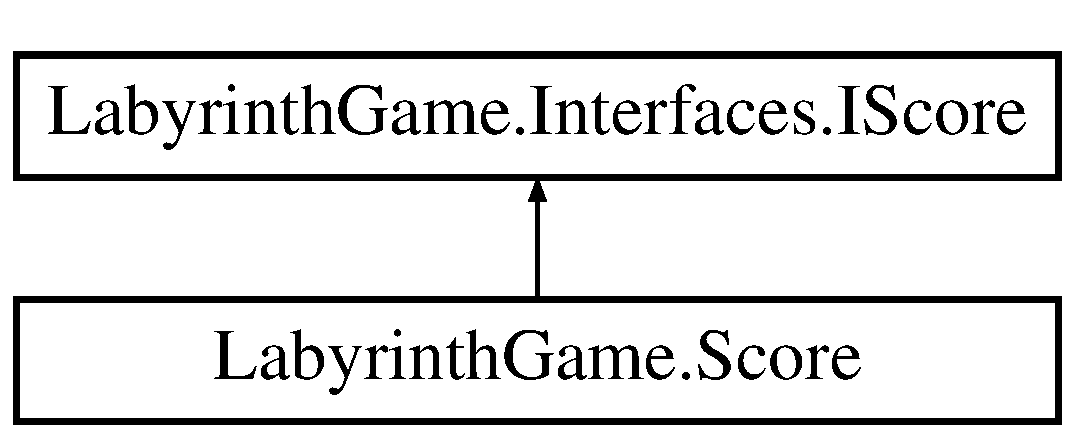
\includegraphics[height=2.000000cm]{interface_labyrinth_game_1_1_interfaces_1_1_i_score}
\end{center}
\end{figure}
\subsection*{Public Member Functions}
\begin{DoxyCompactItemize}
\item 
\hypertarget{interface_labyrinth_game_1_1_interfaces_1_1_i_score_adbb9c4d1b98d5c198bb4bad7af6ffa32}{void {\bfseries Print\+Score\+Board} ()}\label{interface_labyrinth_game_1_1_interfaces_1_1_i_score_adbb9c4d1b98d5c198bb4bad7af6ffa32}

\item 
\hypertarget{interface_labyrinth_game_1_1_interfaces_1_1_i_score_a7f58318fb964f105a7dc3f9020e07822}{void {\bfseries Add\+Score} (\hyperlink{interface_labyrinth_game_1_1_interfaces_1_1_i_player}{I\+Player} player)}\label{interface_labyrinth_game_1_1_interfaces_1_1_i_score_a7f58318fb964f105a7dc3f9020e07822}

\end{DoxyCompactItemize}
\subsection*{Properties}
\begin{DoxyCompactItemize}
\item 
\hypertarget{interface_labyrinth_game_1_1_interfaces_1_1_i_score_a5c21c141ce25c24c8b1a388068c9843c}{Sorted\+Dictionary$<$ string, int $>$ {\bfseries Score\+Board}\hspace{0.3cm}{\ttfamily  \mbox{[}get\mbox{]}}}\label{interface_labyrinth_game_1_1_interfaces_1_1_i_score_a5c21c141ce25c24c8b1a388068c9843c}

\end{DoxyCompactItemize}


\subsection{Detailed Description}
Interface which is inherited by the \hyperlink{class_labyrinth_game_1_1_score}{Score} class 



Definition at line 10 of file I\+Score.\+cs.



The documentation for this interface was generated from the following file\+:\begin{DoxyCompactItemize}
\item 
Labyrinth\+Game/\+Interfaces/I\+Score.\+cs\end{DoxyCompactItemize}

\hypertarget{interface_labyrinth_game_1_1_interfaces_1_1_i_user_command}{\section{Labyrinth\+Game.\+Interfaces.\+I\+User\+Command Interface Reference}
\label{interface_labyrinth_game_1_1_interfaces_1_1_i_user_command}\index{Labyrinth\+Game.\+Interfaces.\+I\+User\+Command@{Labyrinth\+Game.\+Interfaces.\+I\+User\+Command}}
}


Interface which is inherited from the \hyperlink{class_labyrinth_game_1_1_keyboard_command}{Keyboard\+Command}  


Inheritance diagram for Labyrinth\+Game.\+Interfaces.\+I\+User\+Command\+:\begin{figure}[H]
\begin{center}
\leavevmode
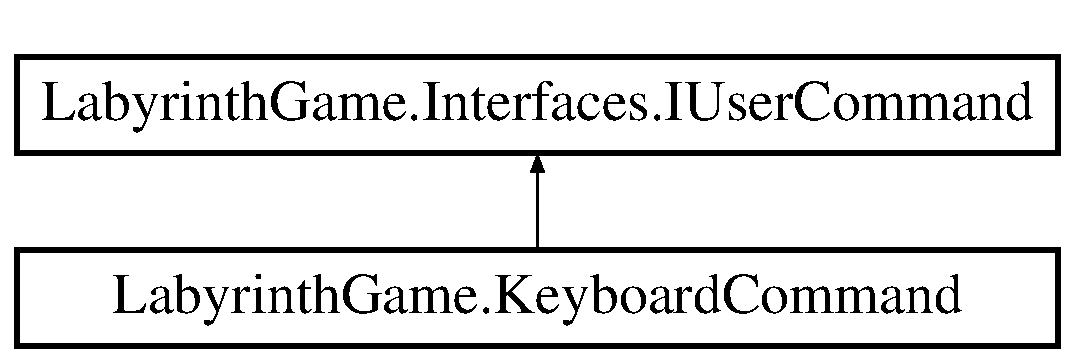
\includegraphics[height=2.000000cm]{interface_labyrinth_game_1_1_interfaces_1_1_i_user_command}
\end{center}
\end{figure}
\subsection*{Public Member Functions}
\begin{DoxyCompactItemize}
\item 
\hypertarget{interface_labyrinth_game_1_1_interfaces_1_1_i_user_command_af7290f1ddd9f104ce8682764a235b84a}{\hyperlink{interface_labyrinth_game_1_1_interfaces_1_1_i_coordinate}{I\+Coordinate} {\bfseries Move\+Left} ()}\label{interface_labyrinth_game_1_1_interfaces_1_1_i_user_command_af7290f1ddd9f104ce8682764a235b84a}

\item 
\hypertarget{interface_labyrinth_game_1_1_interfaces_1_1_i_user_command_a5adeb887ce5d90fc23d15a957fb81856}{\hyperlink{interface_labyrinth_game_1_1_interfaces_1_1_i_coordinate}{I\+Coordinate} {\bfseries Move\+Right} ()}\label{interface_labyrinth_game_1_1_interfaces_1_1_i_user_command_a5adeb887ce5d90fc23d15a957fb81856}

\item 
\hypertarget{interface_labyrinth_game_1_1_interfaces_1_1_i_user_command_a5a2b9bbe219e998aa2f152961aea82f9}{\hyperlink{interface_labyrinth_game_1_1_interfaces_1_1_i_coordinate}{I\+Coordinate} {\bfseries Move\+Down} ()}\label{interface_labyrinth_game_1_1_interfaces_1_1_i_user_command_a5a2b9bbe219e998aa2f152961aea82f9}

\item 
\hypertarget{interface_labyrinth_game_1_1_interfaces_1_1_i_user_command_a18e6cd19052eea0e057489697d783a18}{\hyperlink{interface_labyrinth_game_1_1_interfaces_1_1_i_coordinate}{I\+Coordinate} {\bfseries Move\+Up} ()}\label{interface_labyrinth_game_1_1_interfaces_1_1_i_user_command_a18e6cd19052eea0e057489697d783a18}

\item 
\hypertarget{interface_labyrinth_game_1_1_interfaces_1_1_i_user_command_abf1353ee894d8fbba91d0dbc5aa9d265}{\hyperlink{interface_labyrinth_game_1_1_interfaces_1_1_i_coordinate}{I\+Coordinate} {\bfseries Process\+Commands} ()}\label{interface_labyrinth_game_1_1_interfaces_1_1_i_user_command_abf1353ee894d8fbba91d0dbc5aa9d265}

\end{DoxyCompactItemize}


\subsection{Detailed Description}
Interface which is inherited from the \hyperlink{class_labyrinth_game_1_1_keyboard_command}{Keyboard\+Command} 



Definition at line 9 of file I\+User\+Command.\+cs.



The documentation for this interface was generated from the following file\+:\begin{DoxyCompactItemize}
\item 
Labyrinth\+Game/\+Interfaces/I\+User\+Command.\+cs\end{DoxyCompactItemize}

\hypertarget{class_labyrinth_game_1_1_keyboard_command}{\section{Labyrinth\+Game.\+Keyboard\+Command Class Reference}
\label{class_labyrinth_game_1_1_keyboard_command}\index{Labyrinth\+Game.\+Keyboard\+Command@{Labyrinth\+Game.\+Keyboard\+Command}}
}


The class manages the input from the Engine  


Inheritance diagram for Labyrinth\+Game.\+Keyboard\+Command\+:\begin{figure}[H]
\begin{center}
\leavevmode
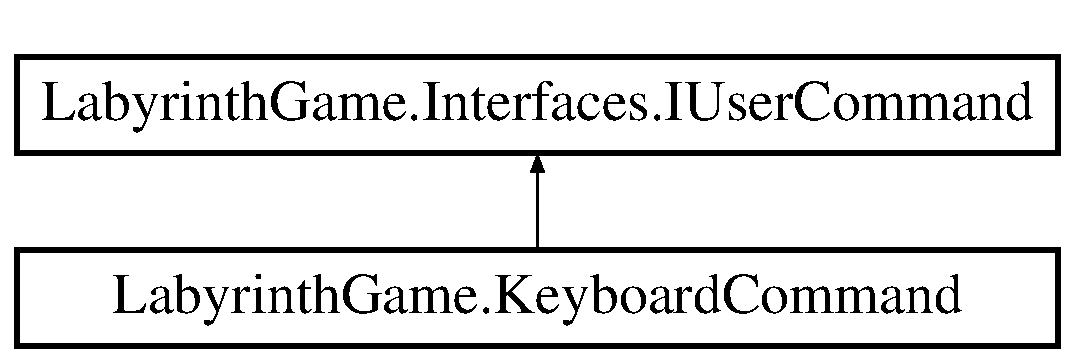
\includegraphics[height=2.000000cm]{class_labyrinth_game_1_1_keyboard_command}
\end{center}
\end{figure}
\subsection*{Public Member Functions}
\begin{DoxyCompactItemize}
\item 
\hyperlink{interface_labyrinth_game_1_1_interfaces_1_1_i_coordinate}{I\+Coordinate} \hyperlink{class_labyrinth_game_1_1_keyboard_command_a19c4c43c956aabf2f1840410e8735cd3}{Move\+Left} ()
\begin{DoxyCompactList}\small\item\em Updates the coordinates and force the objects which use it to move left in a matrix \end{DoxyCompactList}\item 
\hyperlink{interface_labyrinth_game_1_1_interfaces_1_1_i_coordinate}{I\+Coordinate} \hyperlink{class_labyrinth_game_1_1_keyboard_command_a281fa60788d6778b7e157c202574db22}{Move\+Right} ()
\begin{DoxyCompactList}\small\item\em Updates the coordinates and force the objects which use it to move right in a matrix \end{DoxyCompactList}\item 
\hyperlink{interface_labyrinth_game_1_1_interfaces_1_1_i_coordinate}{I\+Coordinate} \hyperlink{class_labyrinth_game_1_1_keyboard_command_af0559dc6b293c70e92f4a49e946c23a3}{Move\+Down} ()
\begin{DoxyCompactList}\small\item\em Updates the coordinates and force the objects which use it to move down in a matrix \end{DoxyCompactList}\item 
\hyperlink{interface_labyrinth_game_1_1_interfaces_1_1_i_coordinate}{I\+Coordinate} \hyperlink{class_labyrinth_game_1_1_keyboard_command_affb746a49aaf2ace462d676046aae8e6}{Move\+Up} ()
\begin{DoxyCompactList}\small\item\em Updates the coordinates and force the objects which use it to move up in a matrix \end{DoxyCompactList}\item 
\hyperlink{interface_labyrinth_game_1_1_interfaces_1_1_i_coordinate}{I\+Coordinate} \hyperlink{class_labyrinth_game_1_1_keyboard_command_a44f06cde013f97e5d35c40485603aab9}{Process\+Commands} ()
\begin{DoxyCompactList}\small\item\em Process the input from the console \end{DoxyCompactList}\end{DoxyCompactItemize}


\subsection{Detailed Description}
The class manages the input from the Engine 



Definition at line 10 of file Keyboard\+Command.\+cs.



\subsection{Member Function Documentation}
\hypertarget{class_labyrinth_game_1_1_keyboard_command_af0559dc6b293c70e92f4a49e946c23a3}{\index{Labyrinth\+Game\+::\+Keyboard\+Command@{Labyrinth\+Game\+::\+Keyboard\+Command}!Move\+Down@{Move\+Down}}
\index{Move\+Down@{Move\+Down}!Labyrinth\+Game\+::\+Keyboard\+Command@{Labyrinth\+Game\+::\+Keyboard\+Command}}
\subsubsection[{Move\+Down}]{\setlength{\rightskip}{0pt plus 5cm}{\bf I\+Coordinate} Labyrinth\+Game.\+Keyboard\+Command.\+Move\+Down (
\begin{DoxyParamCaption}
{}
\end{DoxyParamCaption}
)}}\label{class_labyrinth_game_1_1_keyboard_command_af0559dc6b293c70e92f4a49e946c23a3}


Updates the coordinates and force the objects which use it to move down in a matrix 

\begin{DoxyReturn}{Returns}
Coordinates
\end{DoxyReturn}


Implements \hyperlink{interface_labyrinth_game_1_1_interfaces_1_1_i_user_command}{Labyrinth\+Game.\+Interfaces.\+I\+User\+Command}.



Definition at line 34 of file Keyboard\+Command.\+cs.

\hypertarget{class_labyrinth_game_1_1_keyboard_command_a19c4c43c956aabf2f1840410e8735cd3}{\index{Labyrinth\+Game\+::\+Keyboard\+Command@{Labyrinth\+Game\+::\+Keyboard\+Command}!Move\+Left@{Move\+Left}}
\index{Move\+Left@{Move\+Left}!Labyrinth\+Game\+::\+Keyboard\+Command@{Labyrinth\+Game\+::\+Keyboard\+Command}}
\subsubsection[{Move\+Left}]{\setlength{\rightskip}{0pt plus 5cm}{\bf I\+Coordinate} Labyrinth\+Game.\+Keyboard\+Command.\+Move\+Left (
\begin{DoxyParamCaption}
{}
\end{DoxyParamCaption}
)}}\label{class_labyrinth_game_1_1_keyboard_command_a19c4c43c956aabf2f1840410e8735cd3}


Updates the coordinates and force the objects which use it to move left in a matrix 

\begin{DoxyReturn}{Returns}
Coordinates
\end{DoxyReturn}


Implements \hyperlink{interface_labyrinth_game_1_1_interfaces_1_1_i_user_command}{Labyrinth\+Game.\+Interfaces.\+I\+User\+Command}.



Definition at line 16 of file Keyboard\+Command.\+cs.

\hypertarget{class_labyrinth_game_1_1_keyboard_command_a281fa60788d6778b7e157c202574db22}{\index{Labyrinth\+Game\+::\+Keyboard\+Command@{Labyrinth\+Game\+::\+Keyboard\+Command}!Move\+Right@{Move\+Right}}
\index{Move\+Right@{Move\+Right}!Labyrinth\+Game\+::\+Keyboard\+Command@{Labyrinth\+Game\+::\+Keyboard\+Command}}
\subsubsection[{Move\+Right}]{\setlength{\rightskip}{0pt plus 5cm}{\bf I\+Coordinate} Labyrinth\+Game.\+Keyboard\+Command.\+Move\+Right (
\begin{DoxyParamCaption}
{}
\end{DoxyParamCaption}
)}}\label{class_labyrinth_game_1_1_keyboard_command_a281fa60788d6778b7e157c202574db22}


Updates the coordinates and force the objects which use it to move right in a matrix 

\begin{DoxyReturn}{Returns}
Coordinates
\end{DoxyReturn}


Implements \hyperlink{interface_labyrinth_game_1_1_interfaces_1_1_i_user_command}{Labyrinth\+Game.\+Interfaces.\+I\+User\+Command}.



Definition at line 25 of file Keyboard\+Command.\+cs.

\hypertarget{class_labyrinth_game_1_1_keyboard_command_affb746a49aaf2ace462d676046aae8e6}{\index{Labyrinth\+Game\+::\+Keyboard\+Command@{Labyrinth\+Game\+::\+Keyboard\+Command}!Move\+Up@{Move\+Up}}
\index{Move\+Up@{Move\+Up}!Labyrinth\+Game\+::\+Keyboard\+Command@{Labyrinth\+Game\+::\+Keyboard\+Command}}
\subsubsection[{Move\+Up}]{\setlength{\rightskip}{0pt plus 5cm}{\bf I\+Coordinate} Labyrinth\+Game.\+Keyboard\+Command.\+Move\+Up (
\begin{DoxyParamCaption}
{}
\end{DoxyParamCaption}
)}}\label{class_labyrinth_game_1_1_keyboard_command_affb746a49aaf2ace462d676046aae8e6}


Updates the coordinates and force the objects which use it to move up in a matrix 

\begin{DoxyReturn}{Returns}
Coordinates
\end{DoxyReturn}


Implements \hyperlink{interface_labyrinth_game_1_1_interfaces_1_1_i_user_command}{Labyrinth\+Game.\+Interfaces.\+I\+User\+Command}.



Definition at line 43 of file Keyboard\+Command.\+cs.

\hypertarget{class_labyrinth_game_1_1_keyboard_command_a44f06cde013f97e5d35c40485603aab9}{\index{Labyrinth\+Game\+::\+Keyboard\+Command@{Labyrinth\+Game\+::\+Keyboard\+Command}!Process\+Commands@{Process\+Commands}}
\index{Process\+Commands@{Process\+Commands}!Labyrinth\+Game\+::\+Keyboard\+Command@{Labyrinth\+Game\+::\+Keyboard\+Command}}
\subsubsection[{Process\+Commands}]{\setlength{\rightskip}{0pt plus 5cm}{\bf I\+Coordinate} Labyrinth\+Game.\+Keyboard\+Command.\+Process\+Commands (
\begin{DoxyParamCaption}
{}
\end{DoxyParamCaption}
)}}\label{class_labyrinth_game_1_1_keyboard_command_a44f06cde013f97e5d35c40485603aab9}


Process the input from the console 

\begin{DoxyReturn}{Returns}
returns the four methods for each pressed arrow-\/key\+:\hyperlink{class_labyrinth_game_1_1_keyboard_command_a19c4c43c956aabf2f1840410e8735cd3}{Move\+Left()}, \hyperlink{class_labyrinth_game_1_1_keyboard_command_a281fa60788d6778b7e157c202574db22}{Move\+Right()}, \hyperlink{class_labyrinth_game_1_1_keyboard_command_affb746a49aaf2ace462d676046aae8e6}{Move\+Up()}, \hyperlink{class_labyrinth_game_1_1_keyboard_command_af0559dc6b293c70e92f4a49e946c23a3}{Move\+Down()}
\end{DoxyReturn}


Implements \hyperlink{interface_labyrinth_game_1_1_interfaces_1_1_i_user_command}{Labyrinth\+Game.\+Interfaces.\+I\+User\+Command}.



Definition at line 52 of file Keyboard\+Command.\+cs.



The documentation for this class was generated from the following file\+:\begin{DoxyCompactItemize}
\item 
Labyrinth\+Game/Keyboard\+Command.\+cs\end{DoxyCompactItemize}

\hypertarget{class_labyrinth_game_test_1_1_keyboard_command_test}{\section{Labyrinth\+Game\+Test.\+Keyboard\+Command\+Test Class Reference}
\label{class_labyrinth_game_test_1_1_keyboard_command_test}\index{Labyrinth\+Game\+Test.\+Keyboard\+Command\+Test@{Labyrinth\+Game\+Test.\+Keyboard\+Command\+Test}}
}
\subsection*{Public Member Functions}
\begin{DoxyCompactItemize}
\item 
\hypertarget{class_labyrinth_game_test_1_1_keyboard_command_test_a15a97ba94d8e954a76502662e87bdfbe}{void {\bfseries Move\+Left\+Test\+True} ()}\label{class_labyrinth_game_test_1_1_keyboard_command_test_a15a97ba94d8e954a76502662e87bdfbe}

\item 
\hypertarget{class_labyrinth_game_test_1_1_keyboard_command_test_af2473b77e1565c5998a88cd38b7937ae}{void {\bfseries Move\+Left\+Test\+False} ()}\label{class_labyrinth_game_test_1_1_keyboard_command_test_af2473b77e1565c5998a88cd38b7937ae}

\item 
\hypertarget{class_labyrinth_game_test_1_1_keyboard_command_test_ab0995b8fd2fb9a85233f03b5403b1a26}{void {\bfseries Move\+Right\+Test\+True} ()}\label{class_labyrinth_game_test_1_1_keyboard_command_test_ab0995b8fd2fb9a85233f03b5403b1a26}

\item 
\hypertarget{class_labyrinth_game_test_1_1_keyboard_command_test_a2dbc192d1afd3f2d1cf5f4f6e9700999}{void {\bfseries Move\+Right\+Test\+False} ()}\label{class_labyrinth_game_test_1_1_keyboard_command_test_a2dbc192d1afd3f2d1cf5f4f6e9700999}

\item 
\hypertarget{class_labyrinth_game_test_1_1_keyboard_command_test_a00ffdb95cc681c794ee636e4706e765a}{void {\bfseries Move\+Up\+Test\+True} ()}\label{class_labyrinth_game_test_1_1_keyboard_command_test_a00ffdb95cc681c794ee636e4706e765a}

\item 
\hypertarget{class_labyrinth_game_test_1_1_keyboard_command_test_a69bed30e43c07c451b80b3bbdbbffa85}{void {\bfseries Move\+Up\+Test\+False} ()}\label{class_labyrinth_game_test_1_1_keyboard_command_test_a69bed30e43c07c451b80b3bbdbbffa85}

\item 
\hypertarget{class_labyrinth_game_test_1_1_keyboard_command_test_a616a66be9bd48e07b873791177db8265}{void {\bfseries Move\+Down\+Test\+True} ()}\label{class_labyrinth_game_test_1_1_keyboard_command_test_a616a66be9bd48e07b873791177db8265}

\item 
\hypertarget{class_labyrinth_game_test_1_1_keyboard_command_test_abe676f9f1fbeba9b29903deeb82378a7}{void {\bfseries Move\+Down\+Test\+False} ()}\label{class_labyrinth_game_test_1_1_keyboard_command_test_abe676f9f1fbeba9b29903deeb82378a7}

\end{DoxyCompactItemize}
\subsection*{Static Public Member Functions}
\begin{DoxyCompactItemize}
\item 
\hypertarget{class_labyrinth_game_test_1_1_keyboard_command_test_accb84cddfe4787fb6896649cf0efda02}{static void {\bfseries User\+Command\+Class\+Inicialize} (Test\+Context test\+Context)}\label{class_labyrinth_game_test_1_1_keyboard_command_test_accb84cddfe4787fb6896649cf0efda02}

\end{DoxyCompactItemize}


\subsection{Detailed Description}


Definition at line 9 of file Keyboard\+Command\+Test.\+cs.



The documentation for this class was generated from the following file\+:\begin{DoxyCompactItemize}
\item 
Labyrinth\+Game\+Test/Keyboard\+Command\+Test.\+cs\end{DoxyCompactItemize}

\hypertarget{class_labyrinth_game_1_1_labyrinths_1_1_labyrinth}{\section{Labyrinth\+Game.\+Labyrinths.\+Labyrinth Class Reference}
\label{class_labyrinth_game_1_1_labyrinths_1_1_labyrinth}\index{Labyrinth\+Game.\+Labyrinths.\+Labyrinth@{Labyrinth\+Game.\+Labyrinths.\+Labyrinth}}
}


\hyperlink{class_labyrinth_game_1_1_labyrinths_1_1_labyrinth}{Labyrinth} main logic  


Inheritance diagram for Labyrinth\+Game.\+Labyrinths.\+Labyrinth\+:\begin{figure}[H]
\begin{center}
\leavevmode
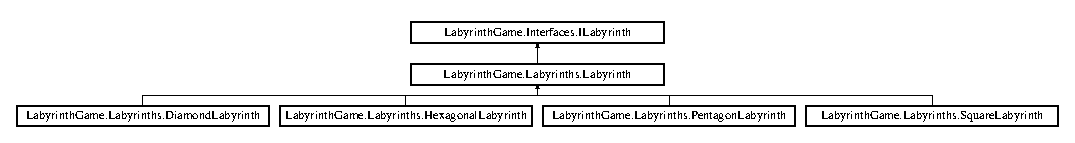
\includegraphics[height=1.473684cm]{class_labyrinth_game_1_1_labyrinths_1_1_labyrinth}
\end{center}
\end{figure}
\subsection*{Public Member Functions}
\begin{DoxyCompactItemize}
\item 
abstract void \hyperlink{class_labyrinth_game_1_1_labyrinths_1_1_labyrinth_a13b3599b7157943b1c028b2f0f5df26c}{Fill\+Matrix} (\hyperlink{interface_labyrinth_game_1_1_interfaces_1_1_i_random_char_provider}{I\+Random\+Char\+Provider} random\+Char\+Provider)
\begin{DoxyCompactList}\small\item\em Creates the char matrix, specific for the different types of labyrinth \end{DoxyCompactList}\item 
virtual void \hyperlink{class_labyrinth_game_1_1_labyrinths_1_1_labyrinth_ac58bba974fe6e9362002b57fbf9816bb}{Change\+Symbol} (\hyperlink{interface_labyrinth_game_1_1_interfaces_1_1_i_coordinate}{I\+Coordinate} coordinates, char new\+Symbol)
\begin{DoxyCompactList}\small\item\em Change symbol at given coordinate position with given new symbol \end{DoxyCompactList}\end{DoxyCompactItemize}
\subsection*{Protected Member Functions}
\begin{DoxyCompactItemize}
\item 
\hyperlink{class_labyrinth_game_1_1_labyrinths_1_1_labyrinth_a0767a92e3dbb0319ad4cf280fde6fe97}{Labyrinth} (\hyperlink{interface_labyrinth_game_1_1_interfaces_1_1_i_renderer}{I\+Renderer} renderer)
\begin{DoxyCompactList}\small\item\em Constructor method \end{DoxyCompactList}\item 
abstract bool \hyperlink{class_labyrinth_game_1_1_labyrinths_1_1_labyrinth_a1f35ce958322025715acf77852f112fa}{Is\+Blank\+Space\+Sign} (int row, int col)
\begin{DoxyCompactList}\small\item\em Checks if sign is Blank\+Space \end{DoxyCompactList}\end{DoxyCompactItemize}
\subsection*{Protected Attributes}
\begin{DoxyCompactItemize}
\item 
\hypertarget{class_labyrinth_game_1_1_labyrinths_1_1_labyrinth_a3ae41ad53bdc67113d3d220982a0a312}{const int {\bfseries Initial\+Rows} = 13}\label{class_labyrinth_game_1_1_labyrinths_1_1_labyrinth_a3ae41ad53bdc67113d3d220982a0a312}

\item 
\hypertarget{class_labyrinth_game_1_1_labyrinths_1_1_labyrinth_afbb8122fcbb44288d15c3ddbe3b7ba54}{const int {\bfseries Initial\+Cols} = 13}\label{class_labyrinth_game_1_1_labyrinths_1_1_labyrinth_afbb8122fcbb44288d15c3ddbe3b7ba54}

\end{DoxyCompactItemize}
\subsection*{Properties}
\begin{DoxyCompactItemize}
\item 
\hypertarget{class_labyrinth_game_1_1_labyrinths_1_1_labyrinth_a7ebf817e69d4183373ee25b8a04a6dc0}{static \hyperlink{interface_labyrinth_game_1_1_interfaces_1_1_i_renderer}{I\+Renderer} {\bfseries Renderer}\hspace{0.3cm}{\ttfamily  \mbox{[}get\mbox{]}}}\label{class_labyrinth_game_1_1_labyrinths_1_1_labyrinth_a7ebf817e69d4183373ee25b8a04a6dc0}

\item 
\hypertarget{class_labyrinth_game_1_1_labyrinths_1_1_labyrinth_afa7a0f7f1a93177ca5b1412bc2053e33}{char\mbox{[},\mbox{]} {\bfseries Matrix}\hspace{0.3cm}{\ttfamily  \mbox{[}get, set\mbox{]}}}\label{class_labyrinth_game_1_1_labyrinths_1_1_labyrinth_afa7a0f7f1a93177ca5b1412bc2053e33}

\end{DoxyCompactItemize}


\subsection{Detailed Description}
\hyperlink{class_labyrinth_game_1_1_labyrinths_1_1_labyrinth}{Labyrinth} main logic 



Definition at line 12 of file Labyrinth.\+cs.



\subsection{Constructor \& Destructor Documentation}
\hypertarget{class_labyrinth_game_1_1_labyrinths_1_1_labyrinth_a0767a92e3dbb0319ad4cf280fde6fe97}{\index{Labyrinth\+Game\+::\+Labyrinths\+::\+Labyrinth@{Labyrinth\+Game\+::\+Labyrinths\+::\+Labyrinth}!Labyrinth@{Labyrinth}}
\index{Labyrinth@{Labyrinth}!Labyrinth\+Game\+::\+Labyrinths\+::\+Labyrinth@{Labyrinth\+Game\+::\+Labyrinths\+::\+Labyrinth}}
\subsubsection[{Labyrinth}]{\setlength{\rightskip}{0pt plus 5cm}Labyrinth\+Game.\+Labyrinths.\+Labyrinth.\+Labyrinth (
\begin{DoxyParamCaption}
\item[{{\bf I\+Renderer}}]{renderer}
\end{DoxyParamCaption}
)\hspace{0.3cm}{\ttfamily [protected]}}}\label{class_labyrinth_game_1_1_labyrinths_1_1_labyrinth_a0767a92e3dbb0319ad4cf280fde6fe97}


Constructor method 


\begin{DoxyParams}{Parameters}
{\em renderer} & I\+Renderer type object\\
\hline
\end{DoxyParams}


Definition at line 25 of file Labyrinth.\+cs.



\subsection{Member Function Documentation}
\hypertarget{class_labyrinth_game_1_1_labyrinths_1_1_labyrinth_ac58bba974fe6e9362002b57fbf9816bb}{\index{Labyrinth\+Game\+::\+Labyrinths\+::\+Labyrinth@{Labyrinth\+Game\+::\+Labyrinths\+::\+Labyrinth}!Change\+Symbol@{Change\+Symbol}}
\index{Change\+Symbol@{Change\+Symbol}!Labyrinth\+Game\+::\+Labyrinths\+::\+Labyrinth@{Labyrinth\+Game\+::\+Labyrinths\+::\+Labyrinth}}
\subsubsection[{Change\+Symbol}]{\setlength{\rightskip}{0pt plus 5cm}virtual void Labyrinth\+Game.\+Labyrinths.\+Labyrinth.\+Change\+Symbol (
\begin{DoxyParamCaption}
\item[{{\bf I\+Coordinate}}]{coordinates, }
\item[{char}]{new\+Symbol}
\end{DoxyParamCaption}
)\hspace{0.3cm}{\ttfamily [virtual]}}}\label{class_labyrinth_game_1_1_labyrinths_1_1_labyrinth_ac58bba974fe6e9362002b57fbf9816bb}


Change symbol at given coordinate position with given new symbol 


\begin{DoxyParams}{Parameters}
{\em coordinates} & We want to change the symbol on the position with this coordinates\\
\hline
{\em new\+Symbol} & This is the symbol we want to put on the given position\\
\hline
\end{DoxyParams}


Implements \hyperlink{interface_labyrinth_game_1_1_interfaces_1_1_i_labyrinth}{Labyrinth\+Game.\+Interfaces.\+I\+Labyrinth}.



Definition at line 72 of file Labyrinth.\+cs.

\hypertarget{class_labyrinth_game_1_1_labyrinths_1_1_labyrinth_a13b3599b7157943b1c028b2f0f5df26c}{\index{Labyrinth\+Game\+::\+Labyrinths\+::\+Labyrinth@{Labyrinth\+Game\+::\+Labyrinths\+::\+Labyrinth}!Fill\+Matrix@{Fill\+Matrix}}
\index{Fill\+Matrix@{Fill\+Matrix}!Labyrinth\+Game\+::\+Labyrinths\+::\+Labyrinth@{Labyrinth\+Game\+::\+Labyrinths\+::\+Labyrinth}}
\subsubsection[{Fill\+Matrix}]{\setlength{\rightskip}{0pt plus 5cm}abstract void Labyrinth\+Game.\+Labyrinths.\+Labyrinth.\+Fill\+Matrix (
\begin{DoxyParamCaption}
\item[{{\bf I\+Random\+Char\+Provider}}]{random\+Char\+Provider}
\end{DoxyParamCaption}
)\hspace{0.3cm}{\ttfamily [pure virtual]}}}\label{class_labyrinth_game_1_1_labyrinths_1_1_labyrinth_a13b3599b7157943b1c028b2f0f5df26c}


Creates the char matrix, specific for the different types of labyrinth 



Implements \hyperlink{interface_labyrinth_game_1_1_interfaces_1_1_i_labyrinth}{Labyrinth\+Game.\+Interfaces.\+I\+Labyrinth}.



Implemented in \hyperlink{class_labyrinth_game_1_1_labyrinths_1_1_hexagonal_labyrinth_af1d2c0c78d13dd85c421ded3dae0a062}{Labyrinth\+Game.\+Labyrinths.\+Hexagonal\+Labyrinth}, \hyperlink{class_labyrinth_game_1_1_labyrinths_1_1_diamond_labyrinth_ae110be09830e8a79d733e37d4916edde}{Labyrinth\+Game.\+Labyrinths.\+Diamond\+Labyrinth}, \hyperlink{class_labyrinth_game_1_1_labyrinths_1_1_pentagon_labyrinth_aa8e799ea6bf80cc6f78eb0d87fa20e93}{Labyrinth\+Game.\+Labyrinths.\+Pentagon\+Labyrinth}, and \hyperlink{class_labyrinth_game_1_1_labyrinths_1_1_square_labyrinth_abd26adbb694f70d8de8eb6239b90ef27}{Labyrinth\+Game.\+Labyrinths.\+Square\+Labyrinth}.

\hypertarget{class_labyrinth_game_1_1_labyrinths_1_1_labyrinth_a1f35ce958322025715acf77852f112fa}{\index{Labyrinth\+Game\+::\+Labyrinths\+::\+Labyrinth@{Labyrinth\+Game\+::\+Labyrinths\+::\+Labyrinth}!Is\+Blank\+Space\+Sign@{Is\+Blank\+Space\+Sign}}
\index{Is\+Blank\+Space\+Sign@{Is\+Blank\+Space\+Sign}!Labyrinth\+Game\+::\+Labyrinths\+::\+Labyrinth@{Labyrinth\+Game\+::\+Labyrinths\+::\+Labyrinth}}
\subsubsection[{Is\+Blank\+Space\+Sign}]{\setlength{\rightskip}{0pt plus 5cm}abstract bool Labyrinth\+Game.\+Labyrinths.\+Labyrinth.\+Is\+Blank\+Space\+Sign (
\begin{DoxyParamCaption}
\item[{int}]{row, }
\item[{int}]{col}
\end{DoxyParamCaption}
)\hspace{0.3cm}{\ttfamily [protected]}, {\ttfamily [pure virtual]}}}\label{class_labyrinth_game_1_1_labyrinths_1_1_labyrinth_a1f35ce958322025715acf77852f112fa}


Checks if sign is Blank\+Space 



Implemented in \hyperlink{class_labyrinth_game_1_1_labyrinths_1_1_hexagonal_labyrinth_a88db5627f18a0a6ebd2b7da78388a925}{Labyrinth\+Game.\+Labyrinths.\+Hexagonal\+Labyrinth}, \hyperlink{class_labyrinth_game_1_1_labyrinths_1_1_diamond_labyrinth_a4a99398d9794ae845d0e9139f69465fe}{Labyrinth\+Game.\+Labyrinths.\+Diamond\+Labyrinth}, \hyperlink{class_labyrinth_game_1_1_labyrinths_1_1_pentagon_labyrinth_a0bcf54dbe004d7d080e62a1b7014a205}{Labyrinth\+Game.\+Labyrinths.\+Pentagon\+Labyrinth}, and \hyperlink{class_labyrinth_game_1_1_labyrinths_1_1_square_labyrinth_af822a30acccb444933b734fe91d9794e}{Labyrinth\+Game.\+Labyrinths.\+Square\+Labyrinth}.



The documentation for this class was generated from the following file\+:\begin{DoxyCompactItemize}
\item 
Labyrinth\+Game/\+Labyrinths/Labyrinth.\+cs\end{DoxyCompactItemize}

\hypertarget{class_labyrinth_game_1_1_labyrinth_creator}{\section{Labyrinth\+Game.\+Labyrinth\+Creator Class Reference}
\label{class_labyrinth_game_1_1_labyrinth_creator}\index{Labyrinth\+Game.\+Labyrinth\+Creator@{Labyrinth\+Game.\+Labyrinth\+Creator}}
}


Labyrinth creator class. Builder pattern used and this class acts as a Director  


Inheritance diagram for Labyrinth\+Game.\+Labyrinth\+Creator\+:\begin{figure}[H]
\begin{center}
\leavevmode
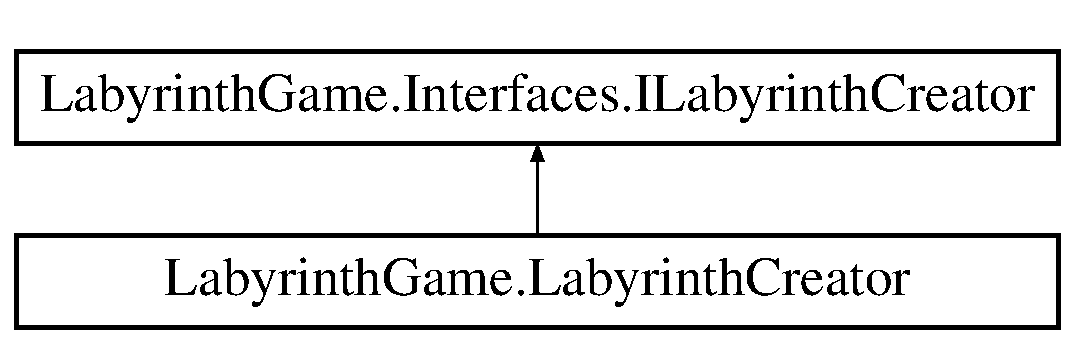
\includegraphics[height=2.000000cm]{class_labyrinth_game_1_1_labyrinth_creator}
\end{center}
\end{figure}
\subsection*{Public Member Functions}
\begin{DoxyCompactItemize}
\item 
\hyperlink{interface_labyrinth_game_1_1_interfaces_1_1_i_labyrinth}{I\+Labyrinth} \hyperlink{class_labyrinth_game_1_1_labyrinth_creator_a5159143053a5877414b8b68561e76a4a}{Create} (string user\+Choice\+Of\+Labyrinth)
\begin{DoxyCompactList}\small\item\em Creates labyrinth of type asked by the user \end{DoxyCompactList}\end{DoxyCompactItemize}


\subsection{Detailed Description}
Labyrinth creator class. Builder pattern used and this class acts as a Director 



Definition at line 13 of file Labyrinth\+Creator.\+cs.



\subsection{Member Function Documentation}
\hypertarget{class_labyrinth_game_1_1_labyrinth_creator_a5159143053a5877414b8b68561e76a4a}{\index{Labyrinth\+Game\+::\+Labyrinth\+Creator@{Labyrinth\+Game\+::\+Labyrinth\+Creator}!Create@{Create}}
\index{Create@{Create}!Labyrinth\+Game\+::\+Labyrinth\+Creator@{Labyrinth\+Game\+::\+Labyrinth\+Creator}}
\subsubsection[{Create}]{\setlength{\rightskip}{0pt plus 5cm}{\bf I\+Labyrinth} Labyrinth\+Game.\+Labyrinth\+Creator.\+Create (
\begin{DoxyParamCaption}
\item[{string}]{user\+Choice\+Of\+Labyrinth}
\end{DoxyParamCaption}
)}}\label{class_labyrinth_game_1_1_labyrinth_creator_a5159143053a5877414b8b68561e76a4a}


Creates labyrinth of type asked by the user 


\begin{DoxyParams}{Parameters}
{\em user\+Choice\+Of\+Labyrinth} & Type of labyrinth asked by user\\
\hline
\end{DoxyParams}
\begin{DoxyReturn}{Returns}
Returns a labyrinth of type as given in parameter with name \char`\"{}user\+Choice\+Of\+Labyrinth\char`\"{}
\end{DoxyReturn}


Implements \hyperlink{interface_labyrinth_game_1_1_interfaces_1_1_i_labyrinth_creator}{Labyrinth\+Game.\+Interfaces.\+I\+Labyrinth\+Creator}.



Definition at line 29 of file Labyrinth\+Creator.\+cs.



The documentation for this class was generated from the following file\+:\begin{DoxyCompactItemize}
\item 
Labyrinth\+Game/Labyrinth\+Creator.\+cs\end{DoxyCompactItemize}

\hypertarget{class_labyrinth_game_test_1_1_labyrinth_creator_test}{\section{Labyrinth\+Game\+Test.\+Labyrinth\+Creator\+Test Class Reference}
\label{class_labyrinth_game_test_1_1_labyrinth_creator_test}\index{Labyrinth\+Game\+Test.\+Labyrinth\+Creator\+Test@{Labyrinth\+Game\+Test.\+Labyrinth\+Creator\+Test}}
}
\subsection*{Public Member Functions}
\begin{DoxyCompactItemize}
\item 
\hypertarget{class_labyrinth_game_test_1_1_labyrinth_creator_test_a7b44a671f9addcd572093aa08bce0ed3}{void {\bfseries Create\+Diamond\+Labyrinth\+Test} ()}\label{class_labyrinth_game_test_1_1_labyrinth_creator_test_a7b44a671f9addcd572093aa08bce0ed3}

\item 
\hypertarget{class_labyrinth_game_test_1_1_labyrinth_creator_test_adb441732990a7c5c95704cd8917ad02e}{void {\bfseries Create\+Hexagonal\+Labyrinth\+Test} ()}\label{class_labyrinth_game_test_1_1_labyrinth_creator_test_adb441732990a7c5c95704cd8917ad02e}

\item 
\hypertarget{class_labyrinth_game_test_1_1_labyrinth_creator_test_adc983be692b3d791c0a7756ceb0fbda4}{void {\bfseries Create\+Pentagon\+Labyrinth\+Test} ()}\label{class_labyrinth_game_test_1_1_labyrinth_creator_test_adc983be692b3d791c0a7756ceb0fbda4}

\item 
\hypertarget{class_labyrinth_game_test_1_1_labyrinth_creator_test_a473a6bb85904c52a08beb61d671e5dc5}{void {\bfseries Create\+Square\+Labyrinth\+Test} ()}\label{class_labyrinth_game_test_1_1_labyrinth_creator_test_a473a6bb85904c52a08beb61d671e5dc5}

\item 
\hypertarget{class_labyrinth_game_test_1_1_labyrinth_creator_test_a74cd5fd550ad201e5b60e3dbf1b5b439}{void {\bfseries Create\+Labyrinth\+Should\+Throw\+Exception\+Test} ()}\label{class_labyrinth_game_test_1_1_labyrinth_creator_test_a74cd5fd550ad201e5b60e3dbf1b5b439}

\end{DoxyCompactItemize}
\subsection*{Static Public Member Functions}
\begin{DoxyCompactItemize}
\item 
\hypertarget{class_labyrinth_game_test_1_1_labyrinth_creator_test_a8dd89a98a55dbf31c81d4be6b97af077}{static void {\bfseries Labyrinth\+Creator\+Class\+Inicialize} (Test\+Context test\+Context)}\label{class_labyrinth_game_test_1_1_labyrinth_creator_test_a8dd89a98a55dbf31c81d4be6b97af077}

\end{DoxyCompactItemize}


\subsection{Detailed Description}


Definition at line 10 of file Labyrinth\+Creator\+Test.\+cs.



The documentation for this class was generated from the following file\+:\begin{DoxyCompactItemize}
\item 
Labyrinth\+Game\+Test/Labyrinth\+Creator\+Test.\+cs\end{DoxyCompactItemize}

\hypertarget{class_labyrinth_game_1_1_labyrinth_engine}{\section{Labyrinth\+Game.\+Labyrinth\+Engine Class Reference}
\label{class_labyrinth_game_1_1_labyrinth_engine}\index{Labyrinth\+Game.\+Labyrinth\+Engine@{Labyrinth\+Game.\+Labyrinth\+Engine}}
}


Singleton implementation of the game engine  


Inheritance diagram for Labyrinth\+Game.\+Labyrinth\+Engine\+:\begin{figure}[H]
\begin{center}
\leavevmode
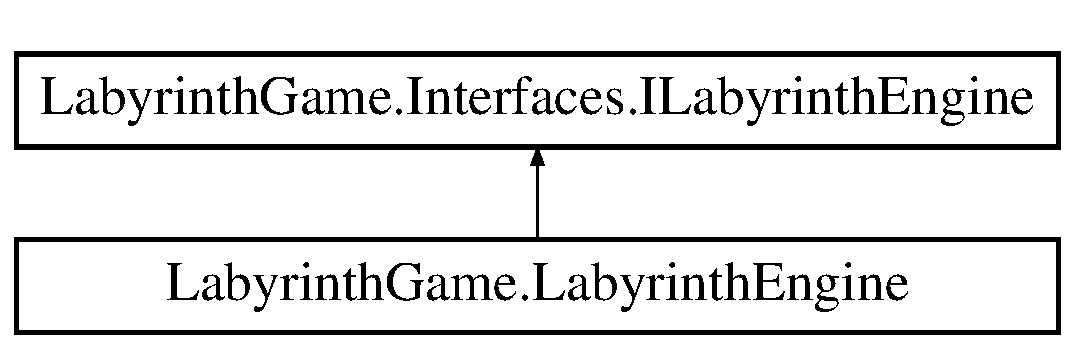
\includegraphics[height=2.000000cm]{class_labyrinth_game_1_1_labyrinth_engine}
\end{center}
\end{figure}
\subsection*{Public Member Functions}
\begin{DoxyCompactItemize}
\item 
void \hyperlink{class_labyrinth_game_1_1_labyrinth_engine_a2ee1c701e5518bc9779c875c93291ccd}{Start} ()
\begin{DoxyCompactList}\small\item\em Start method shows the main menu that asked what \hyperlink{class_labyrinth_game_1_1_player}{Player} want to do, t.\+e play, or restart, or show scoreboard and so on. \end{DoxyCompactList}\end{DoxyCompactItemize}
\subsection*{Properties}
\begin{DoxyCompactItemize}
\item 
\hypertarget{class_labyrinth_game_1_1_labyrinth_engine_a42effc304f6c0e2e9fd4010c3ca65eaa}{static \hyperlink{class_labyrinth_game_1_1_labyrinth_engine}{Labyrinth\+Engine} {\bfseries Instance}\hspace{0.3cm}{\ttfamily  \mbox{[}get\mbox{]}}}\label{class_labyrinth_game_1_1_labyrinth_engine_a42effc304f6c0e2e9fd4010c3ca65eaa}

\item 
\hypertarget{class_labyrinth_game_1_1_labyrinth_engine_a550e4112b72a04de5c4012e424e53a07}{\hyperlink{interface_labyrinth_game_1_1_interfaces_1_1_i_player}{I\+Player} {\bfseries Player}\hspace{0.3cm}{\ttfamily  \mbox{[}get, set\mbox{]}}}\label{class_labyrinth_game_1_1_labyrinth_engine_a550e4112b72a04de5c4012e424e53a07}

\end{DoxyCompactItemize}


\subsection{Detailed Description}
Singleton implementation of the game engine 



Definition at line 11 of file Labyrinth\+Engine.\+cs.



\subsection{Member Function Documentation}
\hypertarget{class_labyrinth_game_1_1_labyrinth_engine_a2ee1c701e5518bc9779c875c93291ccd}{\index{Labyrinth\+Game\+::\+Labyrinth\+Engine@{Labyrinth\+Game\+::\+Labyrinth\+Engine}!Start@{Start}}
\index{Start@{Start}!Labyrinth\+Game\+::\+Labyrinth\+Engine@{Labyrinth\+Game\+::\+Labyrinth\+Engine}}
\subsubsection[{Start}]{\setlength{\rightskip}{0pt plus 5cm}void Labyrinth\+Game.\+Labyrinth\+Engine.\+Start (
\begin{DoxyParamCaption}
{}
\end{DoxyParamCaption}
)}}\label{class_labyrinth_game_1_1_labyrinth_engine_a2ee1c701e5518bc9779c875c93291ccd}


Start method shows the main menu that asked what \hyperlink{class_labyrinth_game_1_1_player}{Player} want to do, t.\+e play, or restart, or show scoreboard and so on. 



Implements \hyperlink{interface_labyrinth_game_1_1_interfaces_1_1_i_labyrinth_engine}{Labyrinth\+Game.\+Interfaces.\+I\+Labyrinth\+Engine}.



Definition at line 52 of file Labyrinth\+Engine.\+cs.



The documentation for this class was generated from the following file\+:\begin{DoxyCompactItemize}
\item 
Labyrinth\+Game/Labyrinth\+Engine.\+cs\end{DoxyCompactItemize}

\hypertarget{class_labyrinth_game_test_1_1_labyrinth_engine_test}{\section{Labyrinth\+Game\+Test.\+Labyrinth\+Engine\+Test Class Reference}
\label{class_labyrinth_game_test_1_1_labyrinth_engine_test}\index{Labyrinth\+Game\+Test.\+Labyrinth\+Engine\+Test@{Labyrinth\+Game\+Test.\+Labyrinth\+Engine\+Test}}
}
\subsection*{Public Member Functions}
\begin{DoxyCompactItemize}
\item 
\hypertarget{class_labyrinth_game_test_1_1_labyrinth_engine_test_af38930f7ec901cf97010ee6c3730b8e5}{void {\bfseries Labyrinth\+Engine\+Is\+Started\+Test} ()}\label{class_labyrinth_game_test_1_1_labyrinth_engine_test_af38930f7ec901cf97010ee6c3730b8e5}

\end{DoxyCompactItemize}
\subsection*{Static Public Member Functions}
\begin{DoxyCompactItemize}
\item 
\hypertarget{class_labyrinth_game_test_1_1_labyrinth_engine_test_a427caaaab82bbff0dd475a72e6d83ef2}{static void {\bfseries Console\+Renderer\+Class\+Inicialize} (Test\+Context test\+Context)}\label{class_labyrinth_game_test_1_1_labyrinth_engine_test_a427caaaab82bbff0dd475a72e6d83ef2}

\end{DoxyCompactItemize}


\subsection{Detailed Description}


Definition at line 10 of file Labyrinth\+Engine\+Test.\+cs.



The documentation for this class was generated from the following file\+:\begin{DoxyCompactItemize}
\item 
Labyrinth\+Game\+Test/Labyrinth\+Engine\+Test.\+cs\end{DoxyCompactItemize}

\hypertarget{class_labyrinth_game_test_1_1_labyrinths_test_1_1_labyrinth_test}{\section{Labyrinth\+Game\+Test.\+Labyrinths\+Test.\+Labyrinth\+Test Class Reference}
\label{class_labyrinth_game_test_1_1_labyrinths_test_1_1_labyrinth_test}\index{Labyrinth\+Game\+Test.\+Labyrinths\+Test.\+Labyrinth\+Test@{Labyrinth\+Game\+Test.\+Labyrinths\+Test.\+Labyrinth\+Test}}
}
\subsection*{Public Member Functions}
\begin{DoxyCompactItemize}
\item 
\hypertarget{class_labyrinth_game_test_1_1_labyrinths_test_1_1_labyrinth_test_aa19311dcd37e3d66e7eaa9da36cc37dd}{void {\bfseries Change\+Symbol\+In\+Square\+Labyrinth\+Test} ()}\label{class_labyrinth_game_test_1_1_labyrinths_test_1_1_labyrinth_test_aa19311dcd37e3d66e7eaa9da36cc37dd}

\item 
\hypertarget{class_labyrinth_game_test_1_1_labyrinths_test_1_1_labyrinth_test_ada01c1e4d52848da2f2cd523f771f1f7}{void {\bfseries Change\+Symbol\+In\+Diamond\+Labyrinth\+Test} ()}\label{class_labyrinth_game_test_1_1_labyrinths_test_1_1_labyrinth_test_ada01c1e4d52848da2f2cd523f771f1f7}

\item 
\hypertarget{class_labyrinth_game_test_1_1_labyrinths_test_1_1_labyrinth_test_a9cbcb41b802b066d1792fc24e06c0091}{void {\bfseries Change\+Symbol\+In\+Hexagonal\+Labyrinth\+Test} ()}\label{class_labyrinth_game_test_1_1_labyrinths_test_1_1_labyrinth_test_a9cbcb41b802b066d1792fc24e06c0091}

\item 
\hypertarget{class_labyrinth_game_test_1_1_labyrinths_test_1_1_labyrinth_test_ad58b363e7814874cbbc70a30e8305793}{void {\bfseries Change\+Symbol\+In\+Pentagon\+Labyrinth\+Test} ()}\label{class_labyrinth_game_test_1_1_labyrinths_test_1_1_labyrinth_test_ad58b363e7814874cbbc70a30e8305793}

\end{DoxyCompactItemize}
\subsection*{Static Public Member Functions}
\begin{DoxyCompactItemize}
\item 
\hypertarget{class_labyrinth_game_test_1_1_labyrinths_test_1_1_labyrinth_test_a8b9705b24584c755c6e10b28a3735185}{static void {\bfseries Console\+Renderer\+Class\+Inicialize} (Test\+Context test\+Context)}\label{class_labyrinth_game_test_1_1_labyrinths_test_1_1_labyrinth_test_a8b9705b24584c755c6e10b28a3735185}

\end{DoxyCompactItemize}


\subsection{Detailed Description}


Definition at line 9 of file Labyrinth\+Test.\+cs.



The documentation for this class was generated from the following file\+:\begin{DoxyCompactItemize}
\item 
Labyrinth\+Game\+Test/\+Labyrinths\+Test/Labyrinth\+Test.\+cs\end{DoxyCompactItemize}

\hypertarget{class_labyrinth_game_1_1_menu}{\section{Labyrinth\+Game.\+Menu Class Reference}
\label{class_labyrinth_game_1_1_menu}\index{Labyrinth\+Game.\+Menu@{Labyrinth\+Game.\+Menu}}
}


The \hyperlink{class_labyrinth_game_1_1_menu}{Menu} class holds the info about the menu of the game  


Inheritance diagram for Labyrinth\+Game.\+Menu\+:\begin{figure}[H]
\begin{center}
\leavevmode
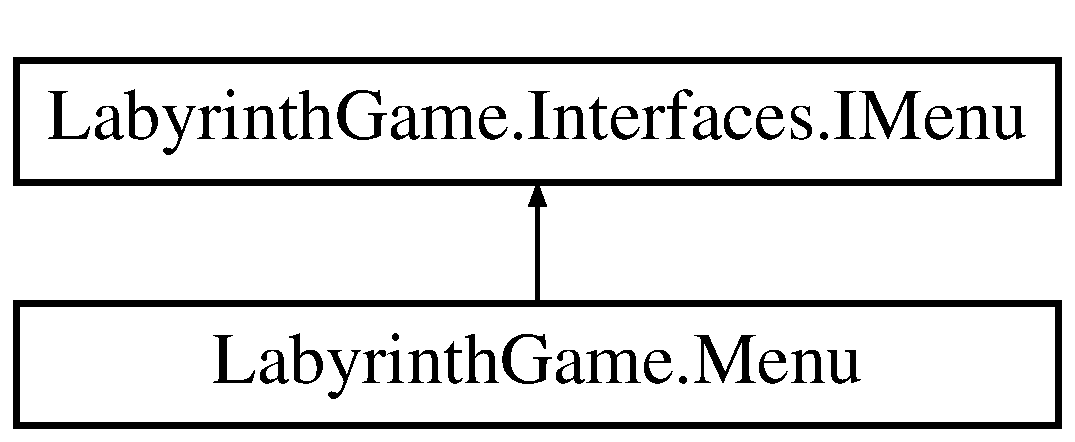
\includegraphics[height=2.000000cm]{class_labyrinth_game_1_1_menu}
\end{center}
\end{figure}
\subsection*{Public Member Functions}
\begin{DoxyCompactItemize}
\item 
string \hyperlink{class_labyrinth_game_1_1_menu_ad23587aa48dd1a0c0ce0774f25d1ca5b}{Get\+User\+Choice} ()
\begin{DoxyCompactList}\small\item\em The method asks user what is his choice of the game -\/ start game, new game, scoreboard or exit of the game \end{DoxyCompactList}\item 
string \hyperlink{class_labyrinth_game_1_1_menu_a48e4db8ff35a86dc421e013cbd986f5e}{Get\+Labyrinth\+Type\+From\+User} ()
\begin{DoxyCompactList}\small\item\em The method asks user what type of labyrinth wants to play -\/ diamond, pentagon, hexagon or square \end{DoxyCompactList}\item 
void \hyperlink{class_labyrinth_game_1_1_menu_ad1afd5a0a2a768cb8657b8f6a4aebda2}{Main\+Menu} ()
\begin{DoxyCompactList}\small\item\em Prints on the console the main menu of the game \end{DoxyCompactList}\item 
\hypertarget{class_labyrinth_game_1_1_menu_a30ae1129b472cba53f84ab34186b791b}{void {\bfseries Menu\+During\+Play} ()}\label{class_labyrinth_game_1_1_menu_a30ae1129b472cba53f84ab34186b791b}

\end{DoxyCompactItemize}


\subsection{Detailed Description}
The \hyperlink{class_labyrinth_game_1_1_menu}{Menu} class holds the info about the menu of the game 



Definition at line 10 of file Menu.\+cs.



\subsection{Member Function Documentation}
\hypertarget{class_labyrinth_game_1_1_menu_a48e4db8ff35a86dc421e013cbd986f5e}{\index{Labyrinth\+Game\+::\+Menu@{Labyrinth\+Game\+::\+Menu}!Get\+Labyrinth\+Type\+From\+User@{Get\+Labyrinth\+Type\+From\+User}}
\index{Get\+Labyrinth\+Type\+From\+User@{Get\+Labyrinth\+Type\+From\+User}!Labyrinth\+Game\+::\+Menu@{Labyrinth\+Game\+::\+Menu}}
\subsubsection[{Get\+Labyrinth\+Type\+From\+User}]{\setlength{\rightskip}{0pt plus 5cm}string Labyrinth\+Game.\+Menu.\+Get\+Labyrinth\+Type\+From\+User (
\begin{DoxyParamCaption}
{}
\end{DoxyParamCaption}
)}}\label{class_labyrinth_game_1_1_menu_a48e4db8ff35a86dc421e013cbd986f5e}


The method asks user what type of labyrinth wants to play -\/ diamond, pentagon, hexagon or square 

\begin{DoxyReturn}{Returns}
Return string that holds the input user choice
\end{DoxyReturn}


Implements \hyperlink{interface_labyrinth_game_1_1_interfaces_1_1_i_menu}{Labyrinth\+Game.\+Interfaces.\+I\+Menu}.



Definition at line 63 of file Menu.\+cs.

\hypertarget{class_labyrinth_game_1_1_menu_ad23587aa48dd1a0c0ce0774f25d1ca5b}{\index{Labyrinth\+Game\+::\+Menu@{Labyrinth\+Game\+::\+Menu}!Get\+User\+Choice@{Get\+User\+Choice}}
\index{Get\+User\+Choice@{Get\+User\+Choice}!Labyrinth\+Game\+::\+Menu@{Labyrinth\+Game\+::\+Menu}}
\subsubsection[{Get\+User\+Choice}]{\setlength{\rightskip}{0pt plus 5cm}string Labyrinth\+Game.\+Menu.\+Get\+User\+Choice (
\begin{DoxyParamCaption}
{}
\end{DoxyParamCaption}
)}}\label{class_labyrinth_game_1_1_menu_ad23587aa48dd1a0c0ce0774f25d1ca5b}


The method asks user what is his choice of the game -\/ start game, new game, scoreboard or exit of the game 

\begin{DoxyReturn}{Returns}
Return string that holds the input user choice
\end{DoxyReturn}


Implements \hyperlink{interface_labyrinth_game_1_1_interfaces_1_1_i_menu}{Labyrinth\+Game.\+Interfaces.\+I\+Menu}.



Definition at line 41 of file Menu.\+cs.

\hypertarget{class_labyrinth_game_1_1_menu_ad1afd5a0a2a768cb8657b8f6a4aebda2}{\index{Labyrinth\+Game\+::\+Menu@{Labyrinth\+Game\+::\+Menu}!Main\+Menu@{Main\+Menu}}
\index{Main\+Menu@{Main\+Menu}!Labyrinth\+Game\+::\+Menu@{Labyrinth\+Game\+::\+Menu}}
\subsubsection[{Main\+Menu}]{\setlength{\rightskip}{0pt plus 5cm}void Labyrinth\+Game.\+Menu.\+Main\+Menu (
\begin{DoxyParamCaption}
{}
\end{DoxyParamCaption}
)}}\label{class_labyrinth_game_1_1_menu_ad1afd5a0a2a768cb8657b8f6a4aebda2}


Prints on the console the main menu of the game 



Implements \hyperlink{interface_labyrinth_game_1_1_interfaces_1_1_i_menu}{Labyrinth\+Game.\+Interfaces.\+I\+Menu}.



Definition at line 82 of file Menu.\+cs.



The documentation for this class was generated from the following file\+:\begin{DoxyCompactItemize}
\item 
Labyrinth\+Game/Menu.\+cs\end{DoxyCompactItemize}

\hypertarget{class_labyrinth_game_test_1_1_menu_test}{\section{Labyrinth\+Game\+Test.\+Menu\+Test Class Reference}
\label{class_labyrinth_game_test_1_1_menu_test}\index{Labyrinth\+Game\+Test.\+Menu\+Test@{Labyrinth\+Game\+Test.\+Menu\+Test}}
}
\subsection*{Public Member Functions}
\begin{DoxyCompactItemize}
\item 
\hypertarget{class_labyrinth_game_test_1_1_menu_test_aa0e27f453254a81aebeb5a42af28641d}{void {\bfseries Menu\+Get\+Choice\+Type\+Diamond\+Test} ()}\label{class_labyrinth_game_test_1_1_menu_test_aa0e27f453254a81aebeb5a42af28641d}

\item 
\hypertarget{class_labyrinth_game_test_1_1_menu_test_a1629560e75f4e655088260f3147b2373}{void {\bfseries Menu\+Get\+Choice\+Type\+Pentagon\+Test} ()}\label{class_labyrinth_game_test_1_1_menu_test_a1629560e75f4e655088260f3147b2373}

\item 
\hypertarget{class_labyrinth_game_test_1_1_menu_test_abbcecbffeff90f67e45a2383b7d9ebc1}{void {\bfseries Menu\+Get\+Choice\+Type\+Hexagon\+Test} ()}\label{class_labyrinth_game_test_1_1_menu_test_abbcecbffeff90f67e45a2383b7d9ebc1}

\item 
\hypertarget{class_labyrinth_game_test_1_1_menu_test_ad46d78ac5a9ee38d3e1751837bf2f803}{void {\bfseries Menu\+Get\+Choice\+Type\+Square\+Test} ()}\label{class_labyrinth_game_test_1_1_menu_test_ad46d78ac5a9ee38d3e1751837bf2f803}

\item 
\hypertarget{class_labyrinth_game_test_1_1_menu_test_ad6d29162f529492326a034a77de9d8d7}{void {\bfseries Menu\+Get\+User\+Choice1\+Test} ()}\label{class_labyrinth_game_test_1_1_menu_test_ad6d29162f529492326a034a77de9d8d7}

\item 
\hypertarget{class_labyrinth_game_test_1_1_menu_test_a869de3700632de4d45add3edd8052c88}{void {\bfseries Menu\+Get\+User\+Choice2\+Test} ()}\label{class_labyrinth_game_test_1_1_menu_test_a869de3700632de4d45add3edd8052c88}

\item 
\hypertarget{class_labyrinth_game_test_1_1_menu_test_acb105bd68e81232c3a7a1766bade610b}{void {\bfseries Menu\+Get\+User\+Choice3\+Test} ()}\label{class_labyrinth_game_test_1_1_menu_test_acb105bd68e81232c3a7a1766bade610b}

\item 
\hypertarget{class_labyrinth_game_test_1_1_menu_test_ad981e2fe5f4a62b9c2cb42845f5ed2e5}{void {\bfseries Menu\+Get\+User\+Choice4\+Test} ()}\label{class_labyrinth_game_test_1_1_menu_test_ad981e2fe5f4a62b9c2cb42845f5ed2e5}

\item 
\hypertarget{class_labyrinth_game_test_1_1_menu_test_ac987aeaee4777f46b96eb638821e65bf}{void {\bfseries Test\+Main\+Menu} ()}\label{class_labyrinth_game_test_1_1_menu_test_ac987aeaee4777f46b96eb638821e65bf}

\item 
\hypertarget{class_labyrinth_game_test_1_1_menu_test_a570bfb5f53160e0bbdcec5c0e08a32a8}{void {\bfseries Test\+Menu\+During\+Play} ()}\label{class_labyrinth_game_test_1_1_menu_test_a570bfb5f53160e0bbdcec5c0e08a32a8}

\end{DoxyCompactItemize}


\subsection{Detailed Description}


Definition at line 9 of file Menu\+Test.\+cs.



The documentation for this class was generated from the following file\+:\begin{DoxyCompactItemize}
\item 
Labyrinth\+Game\+Test/Menu\+Test.\+cs\end{DoxyCompactItemize}

\hypertarget{class_labyrinth_game_1_1_configuration_1_1_ninject_configuration}{\section{Labyrinth\+Game.\+Configuration.\+Ninject\+Configuration Class Reference}
\label{class_labyrinth_game_1_1_configuration_1_1_ninject_configuration}\index{Labyrinth\+Game.\+Configuration.\+Ninject\+Configuration@{Labyrinth\+Game.\+Configuration.\+Ninject\+Configuration}}
}
Inheritance diagram for Labyrinth\+Game.\+Configuration.\+Ninject\+Configuration\+:\begin{figure}[H]
\begin{center}
\leavevmode
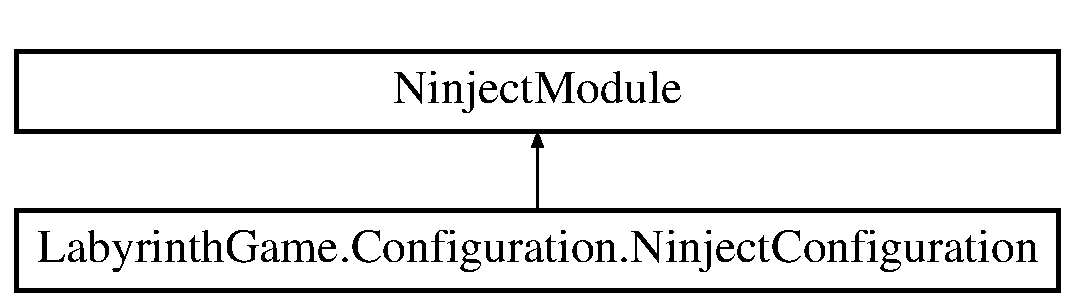
\includegraphics[height=2.000000cm]{class_labyrinth_game_1_1_configuration_1_1_ninject_configuration}
\end{center}
\end{figure}
\subsection*{Public Member Functions}
\begin{DoxyCompactItemize}
\item 
\hypertarget{class_labyrinth_game_1_1_configuration_1_1_ninject_configuration_a339c5ad2cc5702f7b8b8d91a7f5cbd48}{override void {\bfseries Load} ()}\label{class_labyrinth_game_1_1_configuration_1_1_ninject_configuration_a339c5ad2cc5702f7b8b8d91a7f5cbd48}

\end{DoxyCompactItemize}


\subsection{Detailed Description}


Definition at line 6 of file Ninject\+Configuration.\+cs.



The documentation for this class was generated from the following file\+:\begin{DoxyCompactItemize}
\item 
Labyrinth\+Game/\+Configuration/Ninject\+Configuration.\+cs\end{DoxyCompactItemize}

\hypertarget{class_labyrinth_game_1_1_labyrinths_1_1_pentagon_labyrinth}{\section{Labyrinth\+Game.\+Labyrinths.\+Pentagon\+Labyrinth Class Reference}
\label{class_labyrinth_game_1_1_labyrinths_1_1_pentagon_labyrinth}\index{Labyrinth\+Game.\+Labyrinths.\+Pentagon\+Labyrinth@{Labyrinth\+Game.\+Labyrinths.\+Pentagon\+Labyrinth}}
}


Pentagon shaped labyrinth  


Inheritance diagram for Labyrinth\+Game.\+Labyrinths.\+Pentagon\+Labyrinth\+:\begin{figure}[H]
\begin{center}
\leavevmode
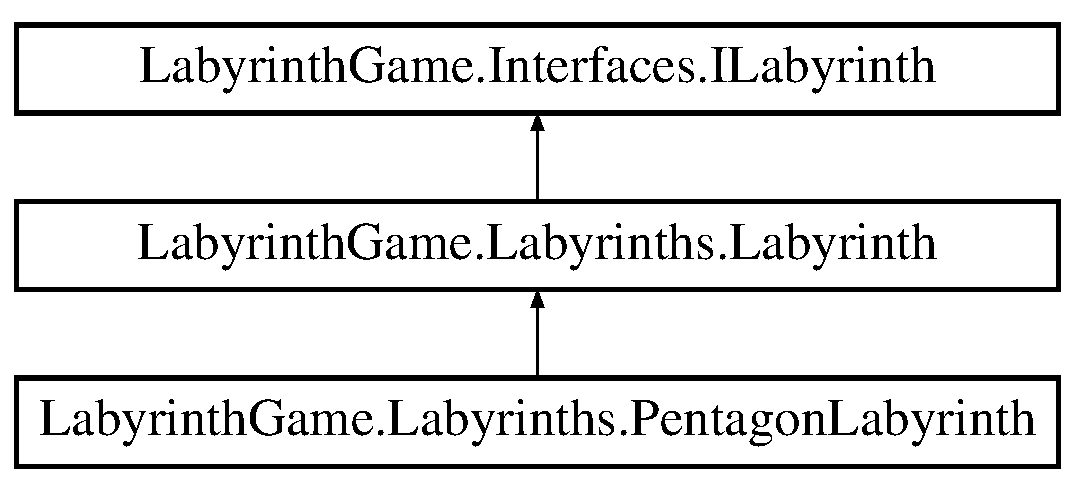
\includegraphics[height=3.000000cm]{class_labyrinth_game_1_1_labyrinths_1_1_pentagon_labyrinth}
\end{center}
\end{figure}
\subsection*{Public Member Functions}
\begin{DoxyCompactItemize}
\item 
\hypertarget{class_labyrinth_game_1_1_labyrinths_1_1_pentagon_labyrinth_a67e8081b5bd87fb878c1570a84b9b631}{{\bfseries Pentagon\+Labyrinth} (\hyperlink{interface_labyrinth_game_1_1_interfaces_1_1_i_renderer}{I\+Renderer} renderer)}\label{class_labyrinth_game_1_1_labyrinths_1_1_pentagon_labyrinth_a67e8081b5bd87fb878c1570a84b9b631}

\item 
override void \hyperlink{class_labyrinth_game_1_1_labyrinths_1_1_pentagon_labyrinth_aa8e799ea6bf80cc6f78eb0d87fa20e93}{Fill\+Matrix} (\hyperlink{interface_labyrinth_game_1_1_interfaces_1_1_i_random_char_provider}{I\+Random\+Char\+Provider} random\+Char\+Provider)
\begin{DoxyCompactList}\small\item\em The method fills the matrix with symbols forming pentagon shape \end{DoxyCompactList}\end{DoxyCompactItemize}
\subsection*{Protected Member Functions}
\begin{DoxyCompactItemize}
\item 
override bool \hyperlink{class_labyrinth_game_1_1_labyrinths_1_1_pentagon_labyrinth_a0bcf54dbe004d7d080e62a1b7014a205}{Is\+Blank\+Space\+Sign} (int row, int col)
\begin{DoxyCompactList}\small\item\em The methods checks if sign is blank-\/space or not \end{DoxyCompactList}\end{DoxyCompactItemize}
\subsection*{Additional Inherited Members}


\subsection{Detailed Description}
Pentagon shaped labyrinth 



Definition at line 9 of file Pentagon\+Labyrinth.\+cs.



\subsection{Member Function Documentation}
\hypertarget{class_labyrinth_game_1_1_labyrinths_1_1_pentagon_labyrinth_aa8e799ea6bf80cc6f78eb0d87fa20e93}{\index{Labyrinth\+Game\+::\+Labyrinths\+::\+Pentagon\+Labyrinth@{Labyrinth\+Game\+::\+Labyrinths\+::\+Pentagon\+Labyrinth}!Fill\+Matrix@{Fill\+Matrix}}
\index{Fill\+Matrix@{Fill\+Matrix}!Labyrinth\+Game\+::\+Labyrinths\+::\+Pentagon\+Labyrinth@{Labyrinth\+Game\+::\+Labyrinths\+::\+Pentagon\+Labyrinth}}
\subsubsection[{Fill\+Matrix}]{\setlength{\rightskip}{0pt plus 5cm}override void Labyrinth\+Game.\+Labyrinths.\+Pentagon\+Labyrinth.\+Fill\+Matrix (
\begin{DoxyParamCaption}
\item[{{\bf I\+Random\+Char\+Provider}}]{random\+Char\+Provider}
\end{DoxyParamCaption}
)\hspace{0.3cm}{\ttfamily [virtual]}}}\label{class_labyrinth_game_1_1_labyrinths_1_1_pentagon_labyrinth_aa8e799ea6bf80cc6f78eb0d87fa20e93}


The method fills the matrix with symbols forming pentagon shape 



Implements \hyperlink{class_labyrinth_game_1_1_labyrinths_1_1_labyrinth_a13b3599b7157943b1c028b2f0f5df26c}{Labyrinth\+Game.\+Labyrinths.\+Labyrinth}.



Definition at line 26 of file Pentagon\+Labyrinth.\+cs.

\hypertarget{class_labyrinth_game_1_1_labyrinths_1_1_pentagon_labyrinth_a0bcf54dbe004d7d080e62a1b7014a205}{\index{Labyrinth\+Game\+::\+Labyrinths\+::\+Pentagon\+Labyrinth@{Labyrinth\+Game\+::\+Labyrinths\+::\+Pentagon\+Labyrinth}!Is\+Blank\+Space\+Sign@{Is\+Blank\+Space\+Sign}}
\index{Is\+Blank\+Space\+Sign@{Is\+Blank\+Space\+Sign}!Labyrinth\+Game\+::\+Labyrinths\+::\+Pentagon\+Labyrinth@{Labyrinth\+Game\+::\+Labyrinths\+::\+Pentagon\+Labyrinth}}
\subsubsection[{Is\+Blank\+Space\+Sign}]{\setlength{\rightskip}{0pt plus 5cm}override bool Labyrinth\+Game.\+Labyrinths.\+Pentagon\+Labyrinth.\+Is\+Blank\+Space\+Sign (
\begin{DoxyParamCaption}
\item[{int}]{row, }
\item[{int}]{col}
\end{DoxyParamCaption}
)\hspace{0.3cm}{\ttfamily [protected]}, {\ttfamily [virtual]}}}\label{class_labyrinth_game_1_1_labyrinths_1_1_pentagon_labyrinth_a0bcf54dbe004d7d080e62a1b7014a205}


The methods checks if sign is blank-\/space or not 


\begin{DoxyParams}{Parameters}
{\em row} & The row we want to check\\
\hline
{\em col} & The column we want to check\\
\hline
\end{DoxyParams}
\begin{DoxyReturn}{Returns}
Returns boolean value -\/ true if it is blank-\/space and false id it is not
\end{DoxyReturn}


Implements \hyperlink{class_labyrinth_game_1_1_labyrinths_1_1_labyrinth_a1f35ce958322025715acf77852f112fa}{Labyrinth\+Game.\+Labyrinths.\+Labyrinth}.



Definition at line 52 of file Pentagon\+Labyrinth.\+cs.



The documentation for this class was generated from the following file\+:\begin{DoxyCompactItemize}
\item 
Labyrinth\+Game/\+Labyrinths/Pentagon\+Labyrinth.\+cs\end{DoxyCompactItemize}

\hypertarget{class_labyrinth_game_test_1_1_labyrinths_test_1_1_pentagon_labyrinth_test}{\section{Labyrinth\+Game\+Test.\+Labyrinths\+Test.\+Pentagon\+Labyrinth\+Test Class Reference}
\label{class_labyrinth_game_test_1_1_labyrinths_test_1_1_pentagon_labyrinth_test}\index{Labyrinth\+Game\+Test.\+Labyrinths\+Test.\+Pentagon\+Labyrinth\+Test@{Labyrinth\+Game\+Test.\+Labyrinths\+Test.\+Pentagon\+Labyrinth\+Test}}
}
\subsection*{Public Member Functions}
\begin{DoxyCompactItemize}
\item 
\hypertarget{class_labyrinth_game_test_1_1_labyrinths_test_1_1_pentagon_labyrinth_test_ad8899b3caedbc54c6a9fa8422127c334}{void {\bfseries Pentagon\+Matrix\+Filled\+Test} ()}\label{class_labyrinth_game_test_1_1_labyrinths_test_1_1_pentagon_labyrinth_test_ad8899b3caedbc54c6a9fa8422127c334}

\end{DoxyCompactItemize}


\subsection{Detailed Description}


Definition at line 11 of file Pentagon\+Labyrinth\+Test.\+cs.



The documentation for this class was generated from the following file\+:\begin{DoxyCompactItemize}
\item 
Labyrinth\+Game\+Test/\+Labyrinths\+Test/Pentagon\+Labyrinth\+Test.\+cs\end{DoxyCompactItemize}

\hypertarget{class_labyrinth_game_1_1_player}{\section{Labyrinth\+Game.\+Player Class Reference}
\label{class_labyrinth_game_1_1_player}\index{Labyrinth\+Game.\+Player@{Labyrinth\+Game.\+Player}}
}


The \hyperlink{class_labyrinth_game_1_1_player}{Player} class hold information about start position, player name and points  


Inheritance diagram for Labyrinth\+Game.\+Player\+:\begin{figure}[H]
\begin{center}
\leavevmode
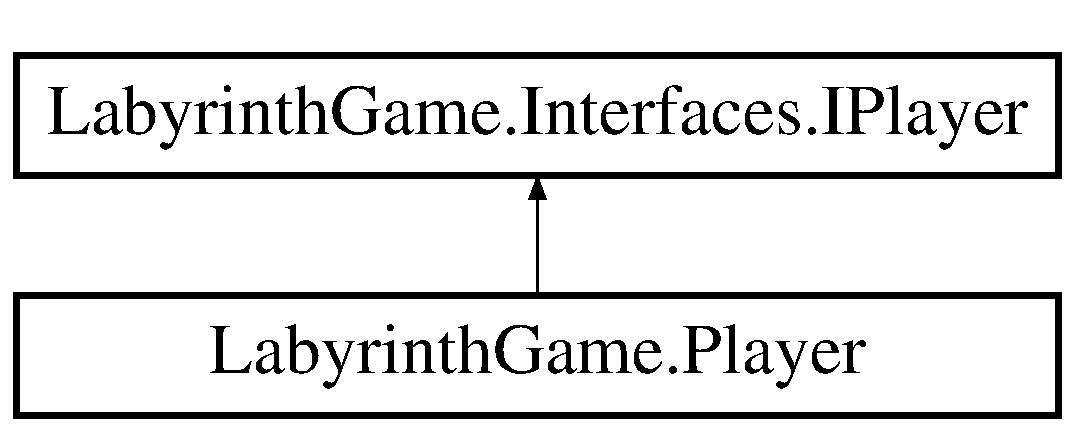
\includegraphics[height=2.000000cm]{class_labyrinth_game_1_1_player}
\end{center}
\end{figure}
\subsection*{Public Member Functions}
\begin{DoxyCompactItemize}
\item 
\hyperlink{class_labyrinth_game_1_1_player_a7d499ce5268336b48d35fc7ba4d10282}{Player} ()
\begin{DoxyCompactList}\small\item\em Constructor \end{DoxyCompactList}\item 
void \hyperlink{class_labyrinth_game_1_1_player_afd1b29af63a3d8b35232e0351be66ec7}{Update\+Points} ()
\begin{DoxyCompactList}\small\item\em The methods calculate the points with every move \end{DoxyCompactList}\item 
void \hyperlink{class_labyrinth_game_1_1_player_a17d185d5d645ca708341a8edda507b39}{Update\+Position} (\hyperlink{interface_labyrinth_game_1_1_interfaces_1_1_i_coordinate}{I\+Coordinate} new\+Coordinates)
\begin{DoxyCompactList}\small\item\em The method updates the position of the player with the given ccorinates \end{DoxyCompactList}\item 
void \hyperlink{class_labyrinth_game_1_1_player_a26d87cb40ba995b3c5a6367f14916b4e}{Show\+Player} (\hyperlink{interface_labyrinth_game_1_1_interfaces_1_1_i_labyrinth}{I\+Labyrinth} labyrinth)
\begin{DoxyCompactList}\small\item\em Puts players sign in the labyrinth \end{DoxyCompactList}\item 
void \hyperlink{class_labyrinth_game_1_1_player_ae995caf4d9b284a112e7b6af8951b647}{Remove\+Player} (\hyperlink{interface_labyrinth_game_1_1_interfaces_1_1_i_labyrinth}{I\+Labyrinth} labyrinth)
\begin{DoxyCompactList}\small\item\em Remove \hyperlink{class_labyrinth_game_1_1_player}{Player} from a position \end{DoxyCompactList}\end{DoxyCompactItemize}
\subsection*{Properties}
\begin{DoxyCompactItemize}
\item 
\hypertarget{class_labyrinth_game_1_1_player_abd56f30d9d6c80f303b858680e747121}{string {\bfseries Name}\hspace{0.3cm}{\ttfamily  \mbox{[}get, set\mbox{]}}}\label{class_labyrinth_game_1_1_player_abd56f30d9d6c80f303b858680e747121}

\item 
\hypertarget{class_labyrinth_game_1_1_player_a3914950908e30f2a3583f2b13565d485}{int {\bfseries Points}\hspace{0.3cm}{\ttfamily  \mbox{[}get, set\mbox{]}}}\label{class_labyrinth_game_1_1_player_a3914950908e30f2a3583f2b13565d485}

\item 
\hypertarget{class_labyrinth_game_1_1_player_a506310cd8dbc411f374cd8d12f309ac7}{\hyperlink{class_labyrinth_game_1_1_coordinate}{Coordinate} {\bfseries Coordinates}\hspace{0.3cm}{\ttfamily  \mbox{[}get, set\mbox{]}}}\label{class_labyrinth_game_1_1_player_a506310cd8dbc411f374cd8d12f309ac7}

\end{DoxyCompactItemize}


\subsection{Detailed Description}
The \hyperlink{class_labyrinth_game_1_1_player}{Player} class hold information about start position, player name and points 



Definition at line 11 of file Player.\+cs.



\subsection{Constructor \& Destructor Documentation}
\hypertarget{class_labyrinth_game_1_1_player_a7d499ce5268336b48d35fc7ba4d10282}{\index{Labyrinth\+Game\+::\+Player@{Labyrinth\+Game\+::\+Player}!Player@{Player}}
\index{Player@{Player}!Labyrinth\+Game\+::\+Player@{Labyrinth\+Game\+::\+Player}}
\subsubsection[{Player}]{\setlength{\rightskip}{0pt plus 5cm}Labyrinth\+Game.\+Player.\+Player (
\begin{DoxyParamCaption}
{}
\end{DoxyParamCaption}
)}}\label{class_labyrinth_game_1_1_player_a7d499ce5268336b48d35fc7ba4d10282}


Constructor 



Definition at line 26 of file Player.\+cs.



\subsection{Member Function Documentation}
\hypertarget{class_labyrinth_game_1_1_player_ae995caf4d9b284a112e7b6af8951b647}{\index{Labyrinth\+Game\+::\+Player@{Labyrinth\+Game\+::\+Player}!Remove\+Player@{Remove\+Player}}
\index{Remove\+Player@{Remove\+Player}!Labyrinth\+Game\+::\+Player@{Labyrinth\+Game\+::\+Player}}
\subsubsection[{Remove\+Player}]{\setlength{\rightskip}{0pt plus 5cm}void Labyrinth\+Game.\+Player.\+Remove\+Player (
\begin{DoxyParamCaption}
\item[{{\bf I\+Labyrinth}}]{labyrinth}
\end{DoxyParamCaption}
)}}\label{class_labyrinth_game_1_1_player_ae995caf4d9b284a112e7b6af8951b647}


Remove \hyperlink{class_labyrinth_game_1_1_player}{Player} from a position 



Implements \hyperlink{interface_labyrinth_game_1_1_interfaces_1_1_i_player}{Labyrinth\+Game.\+Interfaces.\+I\+Player}.



Definition at line 103 of file Player.\+cs.

\hypertarget{class_labyrinth_game_1_1_player_a26d87cb40ba995b3c5a6367f14916b4e}{\index{Labyrinth\+Game\+::\+Player@{Labyrinth\+Game\+::\+Player}!Show\+Player@{Show\+Player}}
\index{Show\+Player@{Show\+Player}!Labyrinth\+Game\+::\+Player@{Labyrinth\+Game\+::\+Player}}
\subsubsection[{Show\+Player}]{\setlength{\rightskip}{0pt plus 5cm}void Labyrinth\+Game.\+Player.\+Show\+Player (
\begin{DoxyParamCaption}
\item[{{\bf I\+Labyrinth}}]{labyrinth}
\end{DoxyParamCaption}
)}}\label{class_labyrinth_game_1_1_player_a26d87cb40ba995b3c5a6367f14916b4e}


Puts players sign in the labyrinth 


\begin{DoxyParams}{Parameters}
{\em labyrinth} & Labyrinth object in which the player should appear \\
\hline
\end{DoxyParams}


Implements \hyperlink{interface_labyrinth_game_1_1_interfaces_1_1_i_player}{Labyrinth\+Game.\+Interfaces.\+I\+Player}.



Definition at line 94 of file Player.\+cs.

\hypertarget{class_labyrinth_game_1_1_player_afd1b29af63a3d8b35232e0351be66ec7}{\index{Labyrinth\+Game\+::\+Player@{Labyrinth\+Game\+::\+Player}!Update\+Points@{Update\+Points}}
\index{Update\+Points@{Update\+Points}!Labyrinth\+Game\+::\+Player@{Labyrinth\+Game\+::\+Player}}
\subsubsection[{Update\+Points}]{\setlength{\rightskip}{0pt plus 5cm}void Labyrinth\+Game.\+Player.\+Update\+Points (
\begin{DoxyParamCaption}
{}
\end{DoxyParamCaption}
)}}\label{class_labyrinth_game_1_1_player_afd1b29af63a3d8b35232e0351be66ec7}


The methods calculate the points with every move 



Implements \hyperlink{interface_labyrinth_game_1_1_interfaces_1_1_i_player}{Labyrinth\+Game.\+Interfaces.\+I\+Player}.



Definition at line 76 of file Player.\+cs.

\hypertarget{class_labyrinth_game_1_1_player_a17d185d5d645ca708341a8edda507b39}{\index{Labyrinth\+Game\+::\+Player@{Labyrinth\+Game\+::\+Player}!Update\+Position@{Update\+Position}}
\index{Update\+Position@{Update\+Position}!Labyrinth\+Game\+::\+Player@{Labyrinth\+Game\+::\+Player}}
\subsubsection[{Update\+Position}]{\setlength{\rightskip}{0pt plus 5cm}void Labyrinth\+Game.\+Player.\+Update\+Position (
\begin{DoxyParamCaption}
\item[{{\bf I\+Coordinate}}]{new\+Coordinates}
\end{DoxyParamCaption}
)}}\label{class_labyrinth_game_1_1_player_a17d185d5d645ca708341a8edda507b39}


The method updates the position of the player with the given ccorinates 


\begin{DoxyParams}{Parameters}
{\em new\+Coordinates} & The coordinates that have to change the players position\\
\hline
\end{DoxyParams}


Implements \hyperlink{interface_labyrinth_game_1_1_interfaces_1_1_i_player}{Labyrinth\+Game.\+Interfaces.\+I\+Player}.



Definition at line 85 of file Player.\+cs.



The documentation for this class was generated from the following file\+:\begin{DoxyCompactItemize}
\item 
Labyrinth\+Game/Player.\+cs\end{DoxyCompactItemize}

\hypertarget{class_labyrinth_game_test_1_1_player_test}{\section{Labyrinth\+Game\+Test.\+Player\+Test Class Reference}
\label{class_labyrinth_game_test_1_1_player_test}\index{Labyrinth\+Game\+Test.\+Player\+Test@{Labyrinth\+Game\+Test.\+Player\+Test}}
}
\subsection*{Public Member Functions}
\begin{DoxyCompactItemize}
\item 
\hypertarget{class_labyrinth_game_test_1_1_player_test_a373be26164636a303e77dae8745f7bbd}{void {\bfseries Get\+Name\+Player\+True} ()}\label{class_labyrinth_game_test_1_1_player_test_a373be26164636a303e77dae8745f7bbd}

\item 
\hypertarget{class_labyrinth_game_test_1_1_player_test_ac52f0c03bc275e7e7d15753dc44b2fbb}{void {\bfseries Set\+Name\+Player\+Null\+Default\+Result} ()}\label{class_labyrinth_game_test_1_1_player_test_ac52f0c03bc275e7e7d15753dc44b2fbb}

\item 
\hypertarget{class_labyrinth_game_test_1_1_player_test_a3b11462d57fadf777a7b89f8517ccef0}{void {\bfseries Set\+Name\+Player\+With\+Empty\+String\+Result} ()}\label{class_labyrinth_game_test_1_1_player_test_a3b11462d57fadf777a7b89f8517ccef0}

\item 
\hypertarget{class_labyrinth_game_test_1_1_player_test_a0992d32fcd104098f7297527bcf736b7}{void {\bfseries Update\+Points\+True} ()}\label{class_labyrinth_game_test_1_1_player_test_a0992d32fcd104098f7297527bcf736b7}

\item 
\hypertarget{class_labyrinth_game_test_1_1_player_test_ad0f21e81e955dc92818851f3b05124aa}{void {\bfseries Update\+Position1x0\+Row\+Changed\+Test} ()}\label{class_labyrinth_game_test_1_1_player_test_ad0f21e81e955dc92818851f3b05124aa}

\item 
\hypertarget{class_labyrinth_game_test_1_1_player_test_a72fa4a12a1230e0e9474c503f619fd0b}{void {\bfseries Update\+Position0x1\+Row\+Changed\+Test} ()}\label{class_labyrinth_game_test_1_1_player_test_a72fa4a12a1230e0e9474c503f619fd0b}

\item 
\hypertarget{class_labyrinth_game_test_1_1_player_test_a07b921c06a8775c83f0773221e2de4c5}{void {\bfseries Update\+Position0x0\+Row\+Changed\+Test} ()}\label{class_labyrinth_game_test_1_1_player_test_a07b921c06a8775c83f0773221e2de4c5}

\item 
\hypertarget{class_labyrinth_game_test_1_1_player_test_a8beac5b2440dd284e29fddb2a124f2a0}{void {\bfseries Update\+Position\+Negative1x0\+Row\+Changed\+Test} ()}\label{class_labyrinth_game_test_1_1_player_test_a8beac5b2440dd284e29fddb2a124f2a0}

\item 
\hypertarget{class_labyrinth_game_test_1_1_player_test_a4a9766783cbd139b2941b07f9448f1a0}{void {\bfseries Update\+Position0x\+Negatiw1\+Row\+Changed\+Test} ()}\label{class_labyrinth_game_test_1_1_player_test_a4a9766783cbd139b2941b07f9448f1a0}

\item 
\hypertarget{class_labyrinth_game_test_1_1_player_test_ae3b0910d2a59fcf1a17f62358ddfc047}{void {\bfseries Remove\+Player\+True\+Test} ()}\label{class_labyrinth_game_test_1_1_player_test_ae3b0910d2a59fcf1a17f62358ddfc047}

\item 
\hypertarget{class_labyrinth_game_test_1_1_player_test_a6fb3814e5e97a10c3928f85f2929b0e7}{void {\bfseries Show\+Player\+True\+Test} ()}\label{class_labyrinth_game_test_1_1_player_test_a6fb3814e5e97a10c3928f85f2929b0e7}

\end{DoxyCompactItemize}


\subsection{Detailed Description}


Definition at line 11 of file Player\+Test.\+cs.



The documentation for this class was generated from the following file\+:\begin{DoxyCompactItemize}
\item 
Labyrinth\+Game\+Test/Player\+Test.\+cs\end{DoxyCompactItemize}

\hypertarget{class_labyrinth_game_1_1_random_char_provider}{\section{Labyrinth\+Game.\+Random\+Char\+Provider Class Reference}
\label{class_labyrinth_game_1_1_random_char_provider}\index{Labyrinth\+Game.\+Random\+Char\+Provider@{Labyrinth\+Game.\+Random\+Char\+Provider}}
}
Inheritance diagram for Labyrinth\+Game.\+Random\+Char\+Provider\+:\begin{figure}[H]
\begin{center}
\leavevmode
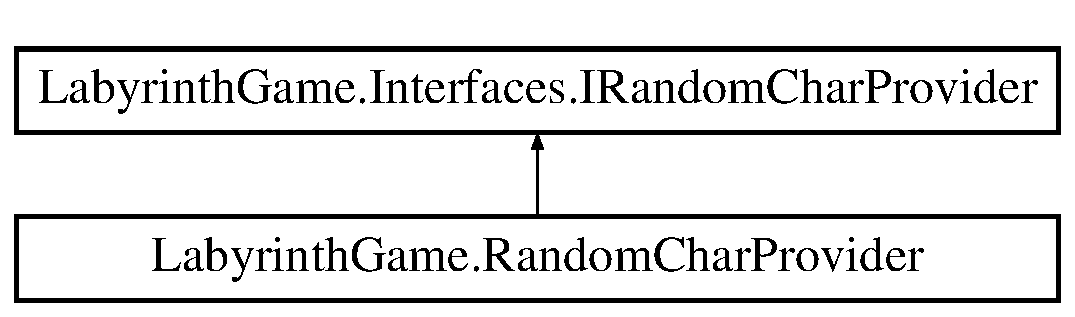
\includegraphics[height=2.000000cm]{class_labyrinth_game_1_1_random_char_provider}
\end{center}
\end{figure}
\subsection*{Public Member Functions}
\begin{DoxyCompactItemize}
\item 
char \hyperlink{class_labyrinth_game_1_1_random_char_provider_a02e6312f17179a4b4cd5dde9cd16ea45}{Get\+Random\+Symbol} (int chance)
\begin{DoxyCompactList}\small\item\em Gives a meaningful symbol depending on a randomly generated value \end{DoxyCompactList}\end{DoxyCompactItemize}


\subsection{Detailed Description}


Definition at line 7 of file Random\+Char\+Provider.\+cs.



\subsection{Member Function Documentation}
\hypertarget{class_labyrinth_game_1_1_random_char_provider_a02e6312f17179a4b4cd5dde9cd16ea45}{\index{Labyrinth\+Game\+::\+Random\+Char\+Provider@{Labyrinth\+Game\+::\+Random\+Char\+Provider}!Get\+Random\+Symbol@{Get\+Random\+Symbol}}
\index{Get\+Random\+Symbol@{Get\+Random\+Symbol}!Labyrinth\+Game\+::\+Random\+Char\+Provider@{Labyrinth\+Game\+::\+Random\+Char\+Provider}}
\subsubsection[{Get\+Random\+Symbol}]{\setlength{\rightskip}{0pt plus 5cm}char Labyrinth\+Game.\+Random\+Char\+Provider.\+Get\+Random\+Symbol (
\begin{DoxyParamCaption}
\item[{int}]{chance}
\end{DoxyParamCaption}
)}}\label{class_labyrinth_game_1_1_random_char_provider_a02e6312f17179a4b4cd5dde9cd16ea45}


Gives a meaningful symbol depending on a randomly generated value 

\begin{DoxyReturn}{Returns}
A symbol
\end{DoxyReturn}


Implements \hyperlink{interface_labyrinth_game_1_1_interfaces_1_1_i_random_char_provider}{Labyrinth\+Game.\+Interfaces.\+I\+Random\+Char\+Provider}.



Definition at line 20 of file Random\+Char\+Provider.\+cs.



The documentation for this class was generated from the following file\+:\begin{DoxyCompactItemize}
\item 
Labyrinth\+Game/Random\+Char\+Provider.\+cs\end{DoxyCompactItemize}

\hypertarget{class_labyrinth_game_test_1_1_random_char_provider_test}{\section{Labyrinth\+Game\+Test.\+Random\+Char\+Provider\+Test Class Reference}
\label{class_labyrinth_game_test_1_1_random_char_provider_test}\index{Labyrinth\+Game\+Test.\+Random\+Char\+Provider\+Test@{Labyrinth\+Game\+Test.\+Random\+Char\+Provider\+Test}}
}
\subsection*{Public Member Functions}
\begin{DoxyCompactItemize}
\item 
\hypertarget{class_labyrinth_game_test_1_1_random_char_provider_test_ae3c37381f1e88bb204c252bc4d61c98e}{void {\bfseries Get\+Random\+Symbol\+Mocked\+Test} ()}\label{class_labyrinth_game_test_1_1_random_char_provider_test_ae3c37381f1e88bb204c252bc4d61c98e}

\item 
\hypertarget{class_labyrinth_game_test_1_1_random_char_provider_test_a4b3beecdafebbced77fb01116b023750}{void {\bfseries Get\+Random\+Symbol\+Returns\+Obstacle\+Test} ()}\label{class_labyrinth_game_test_1_1_random_char_provider_test_a4b3beecdafebbced77fb01116b023750}

\item 
\hypertarget{class_labyrinth_game_test_1_1_random_char_provider_test_a28dafef4f81ce5d13f0bc36ac7350bdb}{void {\bfseries Get\+Random\+Symbol\+Returns\+Path\+Test} ()}\label{class_labyrinth_game_test_1_1_random_char_provider_test_a28dafef4f81ce5d13f0bc36ac7350bdb}

\end{DoxyCompactItemize}


\subsection{Detailed Description}


Definition at line 11 of file Random\+Char\+Provider\+Test.\+cs.



The documentation for this class was generated from the following file\+:\begin{DoxyCompactItemize}
\item 
Labyrinth\+Game\+Test/Random\+Char\+Provider\+Test.\+cs\end{DoxyCompactItemize}

\hypertarget{class_labyrinth_game_1_1_score}{\section{Labyrinth\+Game.\+Score Class Reference}
\label{class_labyrinth_game_1_1_score}\index{Labyrinth\+Game.\+Score@{Labyrinth\+Game.\+Score}}
}


\hyperlink{class_labyrinth_game_1_1_score}{Score} class keeps player name and achieved result  


Inheritance diagram for Labyrinth\+Game.\+Score\+:\begin{figure}[H]
\begin{center}
\leavevmode
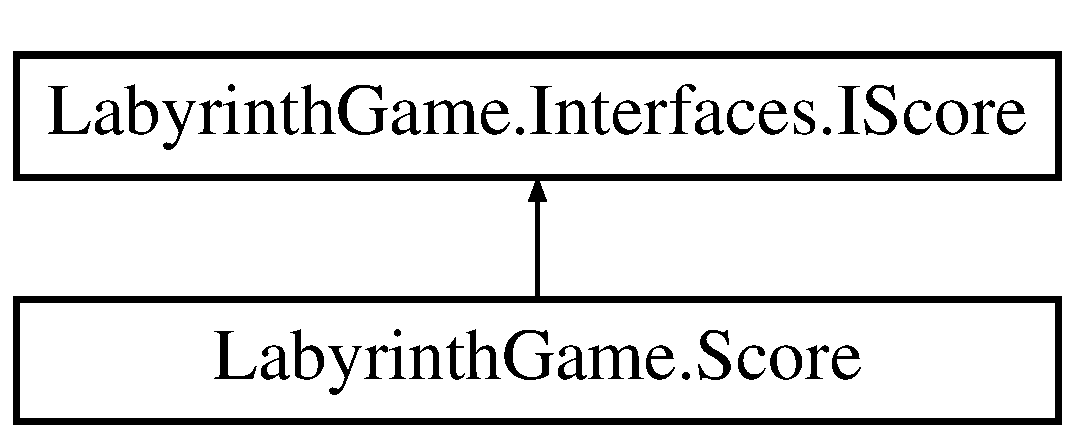
\includegraphics[height=2.000000cm]{class_labyrinth_game_1_1_score}
\end{center}
\end{figure}
\subsection*{Public Member Functions}
\begin{DoxyCompactItemize}
\item 
void \hyperlink{class_labyrinth_game_1_1_score_a7f8fff906c41948227a16058b09214a7}{Print\+Score\+Board} ()
\begin{DoxyCompactList}\small\item\em Prints Scoreboard on the console \end{DoxyCompactList}\item 
void \hyperlink{class_labyrinth_game_1_1_score_a264649a0a5a33dee022dc1a94ab85c9f}{Add\+Score} (\hyperlink{interface_labyrinth_game_1_1_interfaces_1_1_i_player}{I\+Player} player)
\begin{DoxyCompactList}\small\item\em Add player to the archive \end{DoxyCompactList}\end{DoxyCompactItemize}
\subsection*{Properties}
\begin{DoxyCompactItemize}
\item 
\hypertarget{class_labyrinth_game_1_1_score_aaab58f26ea38d8ec62481ea04503753a}{static \hyperlink{class_labyrinth_game_1_1_score}{Score} {\bfseries Score\+Instance}\hspace{0.3cm}{\ttfamily  \mbox{[}get\mbox{]}}}\label{class_labyrinth_game_1_1_score_aaab58f26ea38d8ec62481ea04503753a}

\item 
\hypertarget{class_labyrinth_game_1_1_score_a52d40b8e5b17e6fc7e8a62b63072c6aa}{Sorted\+Dictionary$<$ string, int $>$ {\bfseries Score\+Board}\hspace{0.3cm}{\ttfamily  \mbox{[}get, set\mbox{]}}}\label{class_labyrinth_game_1_1_score_a52d40b8e5b17e6fc7e8a62b63072c6aa}

\end{DoxyCompactItemize}


\subsection{Detailed Description}
\hyperlink{class_labyrinth_game_1_1_score}{Score} class keeps player name and achieved result 



Definition at line 11 of file Score.\+cs.



\subsection{Member Function Documentation}
\hypertarget{class_labyrinth_game_1_1_score_a264649a0a5a33dee022dc1a94ab85c9f}{\index{Labyrinth\+Game\+::\+Score@{Labyrinth\+Game\+::\+Score}!Add\+Score@{Add\+Score}}
\index{Add\+Score@{Add\+Score}!Labyrinth\+Game\+::\+Score@{Labyrinth\+Game\+::\+Score}}
\subsubsection[{Add\+Score}]{\setlength{\rightskip}{0pt plus 5cm}void Labyrinth\+Game.\+Score.\+Add\+Score (
\begin{DoxyParamCaption}
\item[{{\bf I\+Player}}]{player}
\end{DoxyParamCaption}
)}}\label{class_labyrinth_game_1_1_score_a264649a0a5a33dee022dc1a94ab85c9f}


Add player to the archive 


\begin{DoxyParams}{Parameters}
{\em player} & The player that has to be added\\
\hline
\end{DoxyParams}


Implements \hyperlink{interface_labyrinth_game_1_1_interfaces_1_1_i_score}{Labyrinth\+Game.\+Interfaces.\+I\+Score}.



Definition at line 58 of file Score.\+cs.

\hypertarget{class_labyrinth_game_1_1_score_a7f8fff906c41948227a16058b09214a7}{\index{Labyrinth\+Game\+::\+Score@{Labyrinth\+Game\+::\+Score}!Print\+Score\+Board@{Print\+Score\+Board}}
\index{Print\+Score\+Board@{Print\+Score\+Board}!Labyrinth\+Game\+::\+Score@{Labyrinth\+Game\+::\+Score}}
\subsubsection[{Print\+Score\+Board}]{\setlength{\rightskip}{0pt plus 5cm}void Labyrinth\+Game.\+Score.\+Print\+Score\+Board (
\begin{DoxyParamCaption}
{}
\end{DoxyParamCaption}
)}}\label{class_labyrinth_game_1_1_score_a7f8fff906c41948227a16058b09214a7}


Prints Scoreboard on the console 



Implements \hyperlink{interface_labyrinth_game_1_1_interfaces_1_1_i_score}{Labyrinth\+Game.\+Interfaces.\+I\+Score}.



Definition at line 36 of file Score.\+cs.



The documentation for this class was generated from the following file\+:\begin{DoxyCompactItemize}
\item 
Labyrinth\+Game/Score.\+cs\end{DoxyCompactItemize}

\hypertarget{class_labyrinth_game_test_1_1_score_test}{\section{Labyrinth\+Game\+Test.\+Score\+Test Class Reference}
\label{class_labyrinth_game_test_1_1_score_test}\index{Labyrinth\+Game\+Test.\+Score\+Test@{Labyrinth\+Game\+Test.\+Score\+Test}}
}
\subsection*{Public Member Functions}
\begin{DoxyCompactItemize}
\item 
\hypertarget{class_labyrinth_game_test_1_1_score_test_a14546ff4308c557d79f8d6689810d2c1}{void {\bfseries Add\+Score\+Player\+One\+Time\+Test} ()}\label{class_labyrinth_game_test_1_1_score_test_a14546ff4308c557d79f8d6689810d2c1}

\item 
\hypertarget{class_labyrinth_game_test_1_1_score_test_ac7559f550b3685409a7ba5450b27514f}{void {\bfseries Add\+Score\+Player\+Two\+Time\+Test} ()}\label{class_labyrinth_game_test_1_1_score_test_ac7559f550b3685409a7ba5450b27514f}

\item 
\hypertarget{class_labyrinth_game_test_1_1_score_test_aa0f72232a1fc868be36b9aba3f4ffdaa}{void {\bfseries Score\+Board\+Contains\+Specific\+Key\+Test} ()}\label{class_labyrinth_game_test_1_1_score_test_aa0f72232a1fc868be36b9aba3f4ffdaa}

\item 
\hypertarget{class_labyrinth_game_test_1_1_score_test_ac741fe17f5c45d462c23d435a0d1ff37}{void {\bfseries Score\+Board\+Contains\+Specific\+Value\+Test} ()}\label{class_labyrinth_game_test_1_1_score_test_ac741fe17f5c45d462c23d435a0d1ff37}

\item 
\hypertarget{class_labyrinth_game_test_1_1_score_test_ad5268a5e3f16d74fd40c764c1a81f74e}{void {\bfseries Print\+Score\+Test} ()}\label{class_labyrinth_game_test_1_1_score_test_ad5268a5e3f16d74fd40c764c1a81f74e}

\end{DoxyCompactItemize}


\subsection{Detailed Description}


Definition at line 10 of file Score\+Test.\+cs.



The documentation for this class was generated from the following file\+:\begin{DoxyCompactItemize}
\item 
Labyrinth\+Game\+Test/Score\+Test.\+cs\end{DoxyCompactItemize}

\hypertarget{class_labyrinth_game_1_1_labyrinths_1_1_square_labyrinth}{\section{Labyrinth\+Game.\+Labyrinths.\+Square\+Labyrinth Class Reference}
\label{class_labyrinth_game_1_1_labyrinths_1_1_square_labyrinth}\index{Labyrinth\+Game.\+Labyrinths.\+Square\+Labyrinth@{Labyrinth\+Game.\+Labyrinths.\+Square\+Labyrinth}}
}


\hyperlink{class_labyrinth_game_1_1_labyrinths_1_1_labyrinth}{Labyrinth} with square shape  


Inheritance diagram for Labyrinth\+Game.\+Labyrinths.\+Square\+Labyrinth\+:\begin{figure}[H]
\begin{center}
\leavevmode
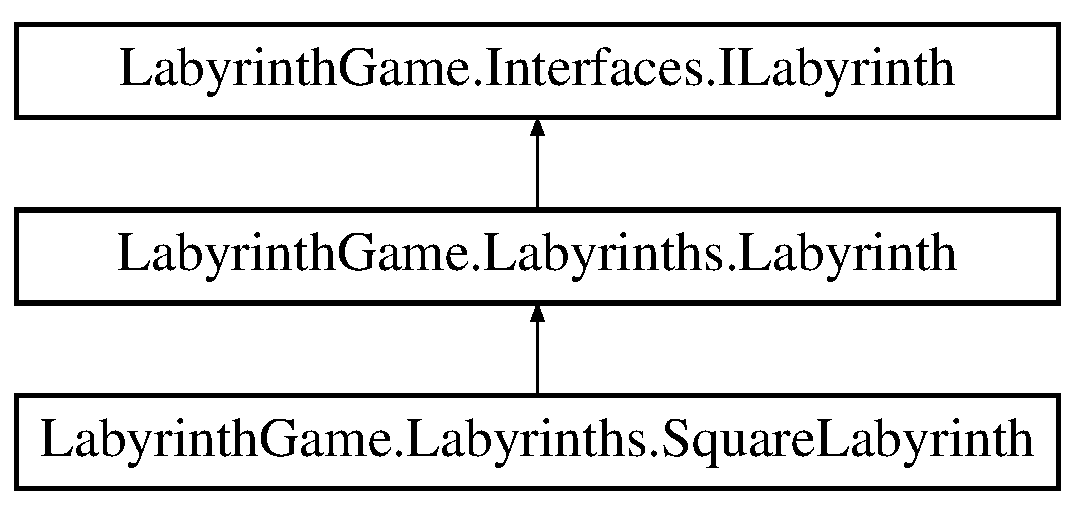
\includegraphics[height=3.000000cm]{class_labyrinth_game_1_1_labyrinths_1_1_square_labyrinth}
\end{center}
\end{figure}
\subsection*{Public Member Functions}
\begin{DoxyCompactItemize}
\item 
\hypertarget{class_labyrinth_game_1_1_labyrinths_1_1_square_labyrinth_a9db3074cf958a1a27556bfe99bc1086f}{{\bfseries Square\+Labyrinth} (\hyperlink{interface_labyrinth_game_1_1_interfaces_1_1_i_renderer}{I\+Renderer} renderer)}\label{class_labyrinth_game_1_1_labyrinths_1_1_square_labyrinth_a9db3074cf958a1a27556bfe99bc1086f}

\item 
override void \hyperlink{class_labyrinth_game_1_1_labyrinths_1_1_square_labyrinth_abd26adbb694f70d8de8eb6239b90ef27}{Fill\+Matrix} (\hyperlink{interface_labyrinth_game_1_1_interfaces_1_1_i_random_char_provider}{I\+Random\+Char\+Provider} random\+Char\+Provider)
\begin{DoxyCompactList}\small\item\em The method fills the matrix with symbols forming square shape \end{DoxyCompactList}\end{DoxyCompactItemize}
\subsection*{Protected Member Functions}
\begin{DoxyCompactItemize}
\item 
override bool \hyperlink{class_labyrinth_game_1_1_labyrinths_1_1_square_labyrinth_af822a30acccb444933b734fe91d9794e}{Is\+Blank\+Space\+Sign} (int row, int col)
\begin{DoxyCompactList}\small\item\em The methods checks if sign is blank-\/space or not \end{DoxyCompactList}\end{DoxyCompactItemize}
\subsection*{Additional Inherited Members}


\subsection{Detailed Description}
\hyperlink{class_labyrinth_game_1_1_labyrinths_1_1_labyrinth}{Labyrinth} with square shape 



Definition at line 8 of file Square\+Labyrinth.\+cs.



\subsection{Member Function Documentation}
\hypertarget{class_labyrinth_game_1_1_labyrinths_1_1_square_labyrinth_abd26adbb694f70d8de8eb6239b90ef27}{\index{Labyrinth\+Game\+::\+Labyrinths\+::\+Square\+Labyrinth@{Labyrinth\+Game\+::\+Labyrinths\+::\+Square\+Labyrinth}!Fill\+Matrix@{Fill\+Matrix}}
\index{Fill\+Matrix@{Fill\+Matrix}!Labyrinth\+Game\+::\+Labyrinths\+::\+Square\+Labyrinth@{Labyrinth\+Game\+::\+Labyrinths\+::\+Square\+Labyrinth}}
\subsubsection[{Fill\+Matrix}]{\setlength{\rightskip}{0pt plus 5cm}override void Labyrinth\+Game.\+Labyrinths.\+Square\+Labyrinth.\+Fill\+Matrix (
\begin{DoxyParamCaption}
\item[{{\bf I\+Random\+Char\+Provider}}]{random\+Char\+Provider}
\end{DoxyParamCaption}
)\hspace{0.3cm}{\ttfamily [virtual]}}}\label{class_labyrinth_game_1_1_labyrinths_1_1_square_labyrinth_abd26adbb694f70d8de8eb6239b90ef27}


The method fills the matrix with symbols forming square shape 



Implements \hyperlink{class_labyrinth_game_1_1_labyrinths_1_1_labyrinth_a13b3599b7157943b1c028b2f0f5df26c}{Labyrinth\+Game.\+Labyrinths.\+Labyrinth}.



Definition at line 23 of file Square\+Labyrinth.\+cs.

\hypertarget{class_labyrinth_game_1_1_labyrinths_1_1_square_labyrinth_af822a30acccb444933b734fe91d9794e}{\index{Labyrinth\+Game\+::\+Labyrinths\+::\+Square\+Labyrinth@{Labyrinth\+Game\+::\+Labyrinths\+::\+Square\+Labyrinth}!Is\+Blank\+Space\+Sign@{Is\+Blank\+Space\+Sign}}
\index{Is\+Blank\+Space\+Sign@{Is\+Blank\+Space\+Sign}!Labyrinth\+Game\+::\+Labyrinths\+::\+Square\+Labyrinth@{Labyrinth\+Game\+::\+Labyrinths\+::\+Square\+Labyrinth}}
\subsubsection[{Is\+Blank\+Space\+Sign}]{\setlength{\rightskip}{0pt plus 5cm}override bool Labyrinth\+Game.\+Labyrinths.\+Square\+Labyrinth.\+Is\+Blank\+Space\+Sign (
\begin{DoxyParamCaption}
\item[{int}]{row, }
\item[{int}]{col}
\end{DoxyParamCaption}
)\hspace{0.3cm}{\ttfamily [protected]}, {\ttfamily [virtual]}}}\label{class_labyrinth_game_1_1_labyrinths_1_1_square_labyrinth_af822a30acccb444933b734fe91d9794e}


The methods checks if sign is blank-\/space or not 


\begin{DoxyParams}{Parameters}
{\em row} & The row we want to check\\
\hline
{\em col} & The column we want to check\\
\hline
\end{DoxyParams}
\begin{DoxyReturn}{Returns}
In that case the matrix does not have blank-\/spaces, so the method throws an exception
\end{DoxyReturn}


Implements \hyperlink{class_labyrinth_game_1_1_labyrinths_1_1_labyrinth_a1f35ce958322025715acf77852f112fa}{Labyrinth\+Game.\+Labyrinths.\+Labyrinth}.



Definition at line 40 of file Square\+Labyrinth.\+cs.



The documentation for this class was generated from the following file\+:\begin{DoxyCompactItemize}
\item 
Labyrinth\+Game/\+Labyrinths/Square\+Labyrinth.\+cs\end{DoxyCompactItemize}

\hypertarget{class_labyrinth_game_test_1_1_labyrinths_test_1_1_square_labyrinth_test}{\section{Labyrinth\+Game\+Test.\+Labyrinths\+Test.\+Square\+Labyrinth\+Test Class Reference}
\label{class_labyrinth_game_test_1_1_labyrinths_test_1_1_square_labyrinth_test}\index{Labyrinth\+Game\+Test.\+Labyrinths\+Test.\+Square\+Labyrinth\+Test@{Labyrinth\+Game\+Test.\+Labyrinths\+Test.\+Square\+Labyrinth\+Test}}
}
\subsection*{Public Member Functions}
\begin{DoxyCompactItemize}
\item 
\hypertarget{class_labyrinth_game_test_1_1_labyrinths_test_1_1_square_labyrinth_test_ab0c07f4be70124c3a64a70bbed3c75c2}{void {\bfseries Square\+Labyrinth\+Fill\+Matrix\+Test} ()}\label{class_labyrinth_game_test_1_1_labyrinths_test_1_1_square_labyrinth_test_ab0c07f4be70124c3a64a70bbed3c75c2}

\end{DoxyCompactItemize}


\subsection{Detailed Description}


Definition at line 11 of file Square\+Labyrinth\+Test.\+cs.



The documentation for this class was generated from the following file\+:\begin{DoxyCompactItemize}
\item 
Labyrinth\+Game\+Test/\+Labyrinths\+Test/Square\+Labyrinth\+Test.\+cs\end{DoxyCompactItemize}

%--- End generated contents ---

% Index
\newpage
\phantomsection
\addcontentsline{toc}{chapter}{Index}
\printindex

\end{document}
